\documentclass[12pt]{article}
\usepackage[margin=1in]{geometry}
%\usepackage{hyperref}
\usepackage{amsmath}
\usepackage{graphicx}% http://ctan.org/pkg/graphicx
\usepackage{systeme}
%% tables
\usepackage{booktabs}
\usepackage[table,xcdraw]{xcolor}
\usepackage{float}

%% Make red text
\newcommand{\com}[1]{\textcolor{red}{ #1}}

%\linespread{2}

\usepackage[authoryear]{natbib}


\usepackage{tikz}
\tikzset{
  int/.style={circle, draw, fill=blue!20, minimum size=3em},
  init/.style={pin distance=1.2cm,pin edge={loop,thin,black}}
}
\usetikzlibrary{arrows,automata}

\pagenumbering{arabic}

\newcommand{\XX}{\ensuremath{25}} % number of methods

\newcommand{\xxsir}{\ensuremath{11}} % number of SIR methods

\newcommand{\rr}{\ensuremath{\mathcal{R}_0}}

\setlength{\itemsep}{0pt}






\begin{document}

%%% draw a tree
\tikzset{
  treenode/.style = {shape=rectangle, rounded corners,
                     draw, align=center,
                     top color=white, bottom color=blue!20},
  root/.style     = {treenode, font=\Large, bottom color=red!30},
  env/.style      = {treenode, font=\ttfamily\normalsize},
  dummy/.style    = {circle,draw}
}




\title{$\XX$ dubious ways of estimating $\rr$}
\author{ Department of Statistics, Carnegie Mellon University}
\date{\today}
\maketitle

% \tableofcontents


\section{Introduction}\label{sec:intro}
What has been called ``arguably the most important quantity in the study of epidemics'', $\mathcal{R}_0$, the reproduction number (by convention pronounced ``R-naught''), for nearly a century, has been an elusive quantity for epidemic modelers to estimate \citep{Heesterbeek2002}.  Defined by \citet{anderson1992}, $\rr$ is the ``the average number of secondary infections produced when one infected individual is introduced into a host population where everyone is susceptible.''  $\rr$, in some ways, summarizes an entire outbreak of a disease; it  is used to assess whether a disease will break out and what percentage of the population needs to be vaccinated to avoid such an outbreak.  Despite a clear definition of $\rr$, epidemiologists have struggled to create a standard  estimator for $\rr$  \citep{hethcote2000}.  The primary issue in estimating $\rr$ is that the quantity is a \textit{property of the model}, meaning that $\rr$ is dependent not only on the usual noise that comes with statistical modeling but also on a variety of assumptions on how researchers assume a disease is transmitted through a population.

Often, disease models are a part of the ``SI-framework'' pioneered by Kermack and McKendrick in the 1920s \citep{getz2006}.  Here, S and I are known as compartments where S stands for ``susceptible'' and I for ``infected.''  The issue of estimating $\rr$ stems from how individuals are assumed, either implicitly or explicitly, to move from the S compartment to the I compartment and any other compartments that have been introduced such as immune, recovered, dead, or exposed, for example.  One of the simplest models in the SI framework is the SIR model where R stands for a ``recovered'' state where individuals are no longer susceptible to the disease \citep{Kermack700}.  Even in this simplified framework, there is much dispute on how $\rr$ is to be estimated arising from assumptions on how populations intermix, if any intervention has been put in place, or whether disease parameters are constant over time.

Other issues about estimating $\rr$ include mathematical versus statistical approaches (i.e. solving for $\rr$ versus estimating $\rr$), how to estimate the quantity in the presence of types of available data, and when to estimate $\rr$ in a disease's lifetime.  This depends on the ``time constant'' of the disease.  Some diseases like measles progress rapdily, HIV more slowly, prion diseases glacially so.  For instance, if only weekly incidence counts of a disease are available, then we have different methods of estimating $\rr$ available than when we have more data available such as contact networks or the serial interval of a disease.  Another major issue is that since $\rr$ is difficult to estimate in the first place, the estimated variance of the estimated $\rr$ has largely been glossed over or  ignored.  This is especially troubling because we are concerned whether $\rr > 1$, which indicates an outbreak of a disease.  A point estimate is simply not enough to estimate the truth of this inequality.

In short, $\rr$ is an important parameter in epidemiology that is very difficult to estimate.  This, in turn, makes it difficult to compare $\rr$ across different diseases or even different instances of the same disease.  Many of these challenges with estimating $\rr$ and more are summarized and expanded upon by \cite{li2011}.

We review $\XX$ ways to estimate $\rr$ across a number of model assumptions and in the presence of different sources of data.  The title of this manuscript is a reference to a seminal paper by Moler and Van Loan (1978) (and its subsequent update in 2003) in which they discuss ``Nineteen dubious ways to compute the exponential of a matrix'' \citep{moler2003}.  We not only review the methods of estimating  $\rr$ but also include recommendations on when to use the methods as well as introducing techniques which allow estimation the variance.  We compare these estimates, when applicable, in the presence of different data, both simulated and real.

The rest of this manuscript is organized as follows.  In Section \ref{sec:overview}, we introduce the methods in four broad groups: the survival function, compartment models, exponential growth models, and agent-based models.    In Section \ref{sec:details}, we give an overview of each of the methods, what assumptions are used, what data is required, and some of the places the method has been used in the past along with ways in which to estimate the variance of the various methods, when possible.  In Section \ref{sec:results}, for a number of different data sets, we give estimates of $\rr$ for the different methods and their variances over a variety of data sets.  Finally, in Section \ref{sec:dis} we discuss our conclusions and recommendations.  


\section{Overview of $\XX$ Methods to estimate $\rr$}
\label{sec:overview}

In this manuscript, $\XX$ methods were chosen to give a survey of methods for estimating $\rr$.  This is not exhaustive, but these methods were chosen due to historical importance and impact in the field of epidemiology. 

In order to organize the methods for estimating $\rr$, we have chosen four broad classes of estimation methods.  These partitions are meant to be guidelines for distinguishing methods from one another rather than immutable groups.  Many of these methods  fit in many of the groups.  We have chosen the four groups as application of the survival function and its close relatives, classic compartment models, exponential growth assumptions, and estimation from networks.  We list these point estimate methods below in Table \ref{tab:methods} and explain each in detail in Section \ref{sec:details}.  In Table \ref{tab:terms}, we summarize many of the common terms used throughout the document.


% Please add the following required packages to your document preamble:
% \usepackage{booktabs}
% \usepackage[table,xcdraw]{xcolor}
% If you use beamer only pass "xcolor=table" option, i.e. \documentclass[xcolor=table]{beamer}
\begin{table}[h]
  \centering
  \resizebox{\textwidth}{!}{
\begin{tabular}{@{}llll@{}}
\toprule
\textbf{Survival Function}        & \textbf{Compartment Models}            & \textbf{Exponential Growth}                       & \textbf{Networks}        \\ \midrule
Survival Function (SF)            & \textbf{SIR}                           & Exponential Growth (EG)                           & Contact Tracing (CT)     \\
Direct Parameter Estimation (DPE) & - Least Squares (SIR LS)               & Maximum Likelihood of Secondary Infections (MLSI) & Branching Process (BP)   \\
Von Foerster Equations (VFE)      & - Reparameterized LS (SIR ReLS)        & Time Dependent Reproduction Number (TDR)          & Agent-Based Models (ABM) \\
                                  & - Linear Model Approximation (SIR LMA) & Initial Growth and  Final Size (IGFS)             &                          \\
                                  & - LMA, All Time Points (SIR LMAT)      &                                                   &                          \\
                                  & - Max of Data (SIR Max)                &                                                   &                          \\
                                  & - Smooth Max (SIR SMax)                &                                                   &                          \\
                                  & - Incidence-Prevalence Ratio (SIR IPR) &                                                   &                          \\
                                  & - Smooth IPR (SIR SIPR)                &                                                   &                          \\
                                  & - Log Linear (SIR LL)                  &                                                   &                          \\
                                  & - Markov Chain Estimation (SIR MC)     &                                                   &                          \\
                                  & - Sequential Bayes (SIR SB)            &                                                   &                          \\
                                  & SEIR Model (SEIR)                      &                                                   &                          \\
                                  & MSEIR Model (MSEIR)                    &                                                   &                          \\
                                  & Amplifier Model (AMP)                  &                                                   &                          \\
                                  & Next Generation Model (NGM)            &                                                   &                          \\ \bottomrule
\end{tabular}
}
\caption{Table of methods used to estimate $\rr$, divided into four categories.}
\label{tab:methods}
\end{table}

Additionally, we describe  interval estimates for the above methods for estimating $\rr$ in order to better answer the question of whether $\rr > 1$, which implies an outbreak of the disease.  These methods are the delta method and posterior distribution.

% Please add the following required packages to your document preamble:
% \usepackage{booktabs}
\begin{table}[]
\centering
\begin{tabular}{@{}ll@{}}
\toprule
Term        & Meaning                                                                                    \\ \midrule
$\rr$     & reproduction number                                                                        \\
$\mathcal{R}_t$     & effective reproduction number at time $t$                                                  \\
$\beta$     & average rate of infection                                                                  \\
$\gamma$    & average rate of recovery                                                                   \\
$\alpha$    & rate of transfer from exposed to infectious                                                \\
$\delta$    & rate of transfer from immune infant to susceptible                                         \\
$D$         & average duration of an infection                                                           \\
$N$         & population size                                                                            \\
$X(t)$      & number of susceptible individuals at time $t$                                              \\
$Y(t)$      & number of infected individuals at time $t$                                                 \\
$Z(t)$      & number of recovered individuals at time $t$                                                \\
$M(t)$      & number of immune infants at time $t$                                                       \\
$E(t)$      & number of exposed individuals at time $t$                                                  \\
$J(t)$      & incidence at time $t$                                                                      \\
$\omega(t)$ & the time from onset of symptoms in an index case to onset of symptoms in a subsequent case \\
$\mu_\infty$       & percentage of population eventually infected                                               \\
IPR         & incidence to prevalence ratio                                                             \\ \bottomrule
\end{tabular}
\caption{Table of common terms used throughout the document and their meanings}\label{tab:terms}
\end{table}




\section{Details for the $\XX$ methods}
\label{sec:details}
\subsection{Survival function}
\label{sec:direct}

The first set of methods are those of the survival function, which is closely  tied to the history of $\rr$.  The survival function, which originates from the field of demography in the late 1800s, describes how many female offspring a woman would produce \citep{dietz1993estimation}.  In demography, we have
\begin{align*}
\rr = \int_0^\infty p(a) \beta(a) da
\end{align*}
where $p(a)$ denotes the probability of a woman surviving to age $a$ and $\beta(a)$ the rate of an individual of age $a$ giving birth to a  girl.   This interpretation also explains the origins of the name of $\rr$, which was imported to the field of epidemiology by MacDonald and Smith \citep{dietz1993estimation}.  Analogously in epidemiology, $p(a)$ is the age of a disease, and $\beta$ is the transmission rate.

This is the chronologically first, and in many ways, the most direct method to estimate $\rr$.  However, this model also seems to be the most difficult to estimate as both $p(a)$ and $\beta (a)$ are random variables.   In general, it is also difficult to estimate these parameters before or even during an ongoing disease outbreak.  As such, $\rr$ can only be estimated after an outbreak, which means it cannot be used to determine ongoing prevention strategies.  However, having a post-disease estimation of $\rr$ may be useful for preventing future outbreaks of the disease and aids in comparing the severity of many diseases.  Another advantage of this method is that it is intuitive and independent of assumptions of how the disease is transmitted from person to person.    We describe four methods which estimate $\rr$ from the survival function:  the survival function, direct estimation, and direct parameter estimation.


\subsubsection{Survival Function (SF)}
\label{sec:survival_fxn}
The first method of estimating $\rr$, is not surprisingly, the survival function itself as presented by \cite{Heffernan2005}.  We use standard notation from infectious disease epidemiology.

Let $F(a)$ be the probability that a newly infected individual remains infectious for at least time $a$, and let $b(a)$ be the average number of newly infected individuals that an infectious individual will produce per unit time when infected for total time $a$.  Then $\rr$ is given in Equation (\ref{eq:r0_survivalfxn}),

\begin{align}\label{eq:r0_survivalfxn}
  \rr = \int_0^\infty b(a)F(a)da.
\end{align}

This method presents one of the unique difficulties of estimating $\rr$: that of reconciling generations and time.  $\rr$ tells us about the generations of the disease, meaning an infector and its infected, but not necessarily when the infections occur.  This reconciliation between generations and time is made difficult as the data we have about a disease is often of a temporal nature.  On the other hand, this method is flexible in that this derivation of $\rr$  does not place assumptions on how the disease transmits through a population.  A disadvantage is that data about $F(a)$ and especially $b(a)$ is difficult to collect directly.

Estimating this quantity in Equation \ref{eq:r0_survivalfxn} is hard and, in fact, rarely attempted. It is due to this difficulty that many of the other methods for estimating $\rr$ even exist.  



\subsubsection{Direct Parameter Estimation (DPE)}
\label{sec:dpe}

Direct parameter estimation, an approach for parameters that are readily available to be estimated, is a `plug-in' estimator approach as described by \cite{lipsitch2003} and \cite{dietz1993estimation}.  This method, like the survival function, is highly interpretable.  We assume that we can estimate $\rr$ if we know how many others an individual comes into contact $(k)$, the probability of transmission given contact $(b)$, and how long the disease lasts within an individual $(D)$.  Then $\rr$ is the product of these parameters, 
\begin{align}\label{eq:dpe}
\rr = kbD.
\end{align}
\cite{lipsitch2003} note that directly estimating $\rr$ in such a way may be difficult due to the available data, as in the previous  method.  They instead estimate $\rr$ using the mean serial interval, $\omega$, the time from onset of symptoms in an index case to the onset of symptoms in a subsequent case infected by the index patient in addition to the assumption of exponential growth of infected cases, as a proxy for the duration $D$.  An advantage of this method is that it reduces the problem to three parameters that we can conceivably collect data on.  A disadvantage is that to estimate $\rr$ alone,  data is only used from the initial outbreak of the disease, so often we have a small sample size, resulting in large confidence sets or credible intervals.


%%%%%%%

\subsubsection{Von Foerster Equations (VFE)}
\label{sec:direct-estim-surv}

A derivation of $\rr$ similar to the survival function comes from the idea of the von Foerster equations, which were used to calculate the number of cells in a ``deme,'' a constrained area.  The function $Y(t, \tau)$ calculates the number of cells of age $\tau$ at time $t$ \citep{trucco1965}.  In epidemiology, $Y$ represents the number of infections instead of cells. Letting $Y(t, \tau)$ be the number of infections at time $t$ of age $\tau$, the von Foerster equation is
\begin{align*}
  \frac{\partial Y(t, \tau)}{\partial t} +   \frac{\partial Y(t, \tau)}{\partial \tau} = -  \lambda \cdot n(t, a) ,
\end{align*}
where $Y(t,\tau)$ is the number of people at time $t$ who were infected time $\tau$ ago and $\lambda$ is the loss function, which we assume to be 0, that is no deaths.  The right hand side represents the net loss of cells.  This derivation is based on the ``reasoning that the number of cells which are in the age category $(a, a + \Delta a)$ at time $t$, is equal to $n(t,a) \Delta a$'' \citep{trucco1965}.     \cite{fraser2004factors} derived an expression for $\rr$ from the von Foerster equation and the additional boundary equation
\begin{align*}
  Y(t,0) &= \int_0^t \beta( \tau) Y(t, \tau) d \tau,
\end{align*}
with initial conditions $Y(0,0) = Y_0$ and $Y(t, \tau) = 0$ when $t < \tau$.  Then the reproduction number is given by Equation \ref{eq:vfr0},
\begin{align}\label{eq:vfr0}
\rr &= \int_0^\infty \beta(\tau) d\tau,
\end{align}
 where $\beta (\tau)$ represents the infectiousness at time $\tau$ since the infection.    Again, this model is more mathematical in nature than practical as $\beta (\tau)$ is difficult to estimate.  To estimate $\rr$, \cite{fraser2004factors} make an approximation that $Y(t, \tau) = K(\tau) \exp (rt)$ and further adapt the method to include prevention strategies.  The main function to be estimated is $\beta (\tau)$.  Estimating $\beta (\tau)$ has many of the same issues as trying to estimate $b(a)$ in the survival function in that it is difficult to estimate while the disease is ongoing but is also advantageous in that it does not place assumptions on how the disease is transmitted throughout the population.


%%%%%%%%%%%%%%%



\subsection{Compartment Models}
\label{sec:cms}

First introduced by \cite{Kermack700}, a large and common set of methods used estimate $\rr$ is that of fitting compartment models (CMs) to disease data.  As described in \cite{daley2001epidemic},  CMs model how objects move from one discrete state to another over time.  These models provide an aggregate model of how diseases may be spread throughout a population.  Within the CM framework, we make four essential assumptions,
\begin{enumerate}
\item The compartments are discrete and have no overlap.
\item The transition of objects into and out of compartments is described by a set of known equations, possibly dependent on unknown parameters.
\item The populations mix homogeneously
  \item The number of objects in each compartment at time $t=0$ is known
  \end{enumerate}  


Another common assumption for compartment models, is the law of mass action, a property borrowed from chemistry which says that the mass of the product is proportional to the mass of the reactants.  In epidemiology, this means that the proportion of new infections is proportional to the current  number of susceptible and infected \citep{anderson1992}.  Therefore, the flow of objects from one compartment to another may be dependent on the percentage of objects within one or many of the compartments. 

For disease modelling, all CMs fall into the SI-framework, meaning that there is a susceptible population that may become infected.  Thus, we require there be susceptible and infected compartments but also allow additional compartments such as the recovered state, an exposed latent state, and more.  CMs may either work with continuous or discrete time and \cite{getz2006} remark that there is no preference between the two.  Of course, data is always recorded in discrete time!

In this section, we discuss $15$ different CM-based methods used to estimate $\rr$.  Different model specifications of CMs yield different mathematical derivations of $\rr$.  That is, for example, an SIR model with non-constant population will yield a different mathematical formula for $\rr$ than the SEIR model (here ``E'' stands for exposed) with non-constant population.  The difference in these two models is that the SEIR model has an extra compartment which in turn effects the estimates of transitions from one compartment to another.  That said, even within the same compartment model framework, we can estimate $\rr$ in a variety of ways using statistical techniques.  In fact, we describe $\xxsir$ methods to estimate $\rr$, within the SIR framework alone!  Most of these methods are recipes to estimate parameters within the SIR model and may be extended to other CM frameworks such as the SEIR model.  The final method described in this section, the next generation operator (NGM) is a general method to derive $\rr$ from any valid CM.  A particular advantage to CMs compared to survival function methods is that they are easier to estimate as the data required is typically collected about diseases: namely, incidence counts.  




\subsubsection{SIR Model}
\label{sec:sir-model}

We begin with the most well known CM, the SIR model.   First introduced to epidemiology by  \cite{Kermack700}, the SIR model governs how individuals transition from susceptible, infected, and recovered compartments.  The model is represented graphically in Figure \ref{fig::sir}. 

\begin{figure}[h]
\centering
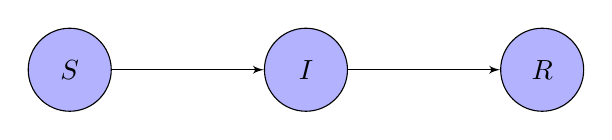
\begin{tikzpicture}[node distance=3cm,auto,>=latex',every node/.append style={align=center}]
    \node [int,  fill = white!70!blue] (a)              {$S$};
    \node [int,  fill = white!70!blue]           (c) [right of=a] {$I$};
    \node [int,  fill = white!70!blue] (e) [right of=c] {$R$};
    \path[->, auto=false] (a) edge node {} (c)
                          (c) edge node {} (e) ;

\end{tikzpicture}
\caption{Depiction of a SIR model.  One can only get the disease once in this model.}\label{fig::sir}
\end{figure}
In this particular  SIR model, $N$, the number of individuals is constant, as we see no arrows pointing away from the three nodes in Figure \ref{fig::sir}. Simple adaptations of the SIR model can include birth and death rates, which may correspondingly change the derivation of $\rr$ (for further discussion, see Section \ref{sec:ngm}). The parameters  $\beta$ and $\gamma$ have epidemiological meaning.  Here, $\beta$ is the average infection rate and $\gamma$ is the average recovery rate.  The transition of individuals from one compartment to another is represented through the ODEs below.  Throughout, we use $X$, $Y$, and $Z$ for stand-ins for the ODEs for $S$, $I$, and $R$, respectively, to avoid any confusion with $\rr$.
\begin{align}
\systeme{\frac{dX}{dt} = -\frac{\beta XY}{N}, \frac{dY}{dt} = \frac{\beta XY}{N} - \gamma Y, \frac{dZ}{dt} = \gamma Z}. \label{eq::sir}
\end{align}

In words, susceptible individuals become infected at a rate that is proportional to the percentage of infected individuals multiplied by $\beta$, the infection rate, and the number of susceptible individuals.  Infected individuals recover at a rate of $\gamma$ multiplied by the number of infected individuals.

An outbreak occurs if the rate of change of infected individuals is positive,
\begin{align*}
  \frac{dY}{dt} &> 0 \\
  \frac{\beta X Y}{N}  - \gamma Y &> 0 ,\\
  Y \left ( \beta \frac{X}{N} - \gamma \right ) & > 0
\end{align*}
that is,  the rate of new infections is greater than the rate of recovery.  So as long as the number of susceptibles is large, $\frac{X}{N} \approx 1$, then an outbreak will occur if $\rr >1$,
\begin{align}\label{eq:deriv_sir}
  \rr = \frac{\beta}{\gamma} > 1.
  \end{align}
Ideally, we have access data of the number of susceptibles, infecteds, and recovered individuals at different points over time.  From this we would like to estimate the $\beta$ and $\gamma$ parameters and ultimately $\rr$.

There are numerous ways to estimate the parameters in this model.  We detail $\xxsir$ of them here.  In every one of these methods, it is assumed that the SIR model is the correct specification.

\subsubsection{Least Squares ($\beta$, $\gamma$) (SIR LS)}\label{least-squares-beta-gamma}
The first approach to estimate $\rr$ in the SIR model is simply to minimize the joint mean square error for the data collected at each time point and use the plug-in estimator found in Equation \ref{eq:sirls}.  In particular, we find

\begin{align*}
(\hat{\beta}, \hat{\gamma} )&=\text{argmin}_{\beta, \gamma} \sum_{t} \left [ \left (Y_{obs}(t) - Y(t)\right )^2 + \left ( X_{obs}(t) - X(t) \right )^2 \right ]
\end{align*}
Then  the estimate for $\rr$ is given by Equation \ref{eq:sirls},
\begin{align}\label{eq:sirls}
  \hat{R}_0= \frac{\hat{\beta}}{\hat{\gamma}}.
  \end{align}
We can use gradient descent or another optimizer to find estimates for these parameters.  If we assume $Y= f(t) + \epsilon_t$ with $\epsilon_t \overset{iid}{\sim} N(0, \sigma^2)$ where $f(t) = \int_0^t \frac{dY}{ds} ds$, then this this method is equivalent to finding the maximum likelihood estimator (MLE) of $\beta$ and $\gamma$.  However, we note that the the $\epsilon_t$ are certainly not independent from one another and so valid inference is still an issue in this framework.  Even if it were correct, ratio estimatiors typically result in large, uninformative confidence intervals.   The advantage is that this is a very straightforward way to estimate $\rr$ from the SIR model.

\subsubsection{Reparametrized Least Squares ($\rr$, $\gamma$) ( SIR ReLS)}\label{reparametrized-least-squares-rux5f0-gamma}

In the previous method, we estimated $\beta$ and $\gamma$ and then estimated $\rr$.  However, it is possible to directly estimate $\rr$ if we reparametrize the ODEs in Equation \eqref{eq::sir} directly with \(\rr\) and \(\gamma\), using the relation $\rr = \frac{\beta}{\gamma}$.

\begin{align*}
  \left \{
  \begin{array}{cl}
    \frac{dX}{dt} &= - \rr \gamma Y \frac{X}{N}\\
    \frac{dY}{dt} &=  \rr \gamma Y \frac{X}{N}  - \gamma Y \\
    \frac{dZ}{dt} &=  - \gamma Y 
  \end{array}
  \right .
  \end{align*}
We find
\begin{align*}
(\hat{R}_0, \hat{\gamma} ) &= \text{argmin}_{\beta, \gamma} \sum_{t} \left [ \left (Y_{obs}(t) - Y(t)\right )^2 + \left ( X_{obs}(t) - X(t) \right )^2 \right ]
\end{align*}
We use the \(\rr\) directly from the above estimation process, which again can be done with gradient descent or another optimization process.  Again, we cannot assume $\rr$ has a normal distribution as the errors are correlated.  This method is better than SIR LS for estimating $\rr$ as there is no ratio.



\subsubsection{Linear Model Approximation (SIR LMA)}\label{linear-model-approximation-degree-10}

The SIR ODEs have no known closed form solution, and so we are already using approximations using numerical integration, albeit small approximations.  In addition to this, data collected from real diseases are typically very noisy in the first place.  \cite{chang2017} discovered that an SIR model may be well approximated by a linear model.  We use this approach here to estimate $\rr$.

Specifically, we fit two linear polynomials in \(t\) with degree \(K= 10\) to \(X_{obs}\)
and \(Y_{obs}\) using least squares to find the coefficients $\{(\hat{x}_k,
\hat{y}_k)\}_{k=1, \dots, K}$,
\begin{align*}
\hat{X}(t) &= \sum_{k=0}^K \hat{x}_k t^k\\
{\hat{Y}}(t) &= \sum_{k=0}^K \hat{y}_k t^k
\end{align*}
Then, we estimate the derivatives as
\begin{align*}
\hat{X}^\prime(t) &= \sum_{k=1}^K k \hat{x}_k t^{k-1}\\
\hat{Y}^\prime(t) &= \sum_{k=0}^K k \hat{y}_k t^{k-1}
\end{align*}
Following,  \(\rr\) is derived from the ODEs in Equation \eqref{eq::sir},
\begin{align}
  - \frac{X^\prime}{Z^\prime}&= \rr \frac{X}{N} \nonumber\\
\rr &=       \frac{X}{ X + Y} \cdot \frac{N}{X} \nonumber\\
  \hat{\rr} &= \frac{\hat{X}^\prime(0)}{ \hat{X}^\prime(0) + \hat{Y}^\prime(0)} \cdot \frac{N}{\hat{X}(0)}. \nonumber
  \end{align}
Like in the previous cases, we are assuming the true models are
\begin{align*}
X(t) &= \sum_{k=0}^K x_k t^k + \epsilon_t\\
  {Y}(t) &= \sum_{k=0}^K y_k t^k + \epsilon_t,
\end{align*}
with $\epsilon_t \overset{iid}{\sim} N(0, \sigma^2)$.  Here, $K=10$ is rather arbitrary and should be selected using some criterion such as AIC in addition with the knowledge of how many data points are available to the user.  Besides optionally deciding on the degree of polynomials to fit, this model is simple to implement and gives very comparable results to using least squares with the SIR model.  The time $t=0$ to best capture the initial outbreak.  Again, we cannot use this model for inference, as our error assumption is violated.  Another disadvantage is that we are using the first time point $t=0$ to estimate $\rr$.  

\subsubsection{Linear Model Approximation, All Time Points (SIR LMAT)}\label{linear-model-approximation-all-time-points-degree-10}

The above formulation of a linear model approximation only uses the estimate at time $t=0$ to estimate $\rr$.  We can instead, use all time points available to estimate $\rr$.  We fit a linear polynomial of \(t\) with degree \(K= 10\) model to \(X\)
and \(Y\) as above, with a slight modification in how we calculate
\(\rr\),
\[\rr = \frac{1}{\# \text{ Obs }t}\sum_t \frac{\hat{X}^\prime(t)}{ \hat{X}^\prime(t) + \hat{Y}^\prime(t)} \cdot \frac{N}{X(0)} \]
The intuition is that $\frac{X^\prime}{X^\prime + Y^\prime}$ is constant in $t$, but due to our approximations with the linear model, this is no longer the case.  Here, we average over the different possible values of $\rr$, estimated at different times.  An advantage to this approach is that we have a more robust estimate of $\rr$ than just using one time point.  The disadvantages are the same as before.

\subsubsection{Max of Data (SIR Max)}\label{max-of-data}
The I ($Y$) compartment of the SIR model has one peak.    We note that \(Y^\prime(t) = \frac{\beta XY}{N} - \gamma Y = 0\) when \(\rr = \frac{\beta}{\gamma} = \frac{N(t)}{X(t)}\). The max
of \(Y\) occurs when \(Y^\prime = 0\) and hence
\[\rr = \frac{N}{X_{obs}(t^*)},\] where
\(t^* = \text{arg max}_{t} Y_{obs}(t)\).   A major disadvantage to this method is that it only uses one sample, making it a highly variable statistic.  An advantage of this method is that it places no distributional assumptions on any parameter.

\subsubsection{Smooth Maximum of Data (SIR SMax)}\label{smooth-maximum-of-data}

We use a spline with 4 degrees of freedom to fit both \(X\), and \(Y\).
We then apply the principle as above, except now,
\[\rr = \frac{N}{\hat{X}(t^*)},\] where
\(t^* = \text{arg max}_{t} \hat{Y}(t)\).   This approach is a statistical approximation of the previous method of using the smoothed max to estimate $\rr$ instead of a single point.  In this way, we can utilize all our data.  Another advantage is the flexibility in model choice in that we can use a spline, linear regression, or any other model which gives us predictions for the number infected and number of susceptibles.  However, despite this flexibility in model choice, one must remember that we assumed an underlying SIR model for the derivation of $\rr$.  Also, it may be unclear how to estimate the variance from this method.

\subsubsection{Incidence to Prevalence
  Ratio (SIR IPR)}\label{incidence-to-prevalence-ratio}
The incidence to prevalence ratio (IPR), described by \cite{Nishiura2009} is another intuitive method to calculate $\rr$ as it incorporates some of the most basic epidemiological quantities, incidence and prevalence.

In terms of data from the SIR model, incidence $J(t) \approx -(X(t+1) - X(t))$, and the IPR$(t) = \frac{J(t)}{Y(t)}$. The \textit{actual} reproduction number, $R_a(t) = \text{IPR}(t)\cdot D$ where $D = 1 /\gamma$ the duration of the infection.  This method assumes that we have some prior knowledge about $\gamma$, the transmission rate.  Thus we use as our estimate,
\begin{align*}
\rr &= \textnormal{IPR}(t) \cdot D
\end{align*}

Here we assume that the time step is small enough to approximate the incidence.  The advantage of this method is that incidence data is generally readily available as is prevalence data for certain diseases such as HIV.  However, as one is required to have prior knowledge about $\gamma$, it may be easier to directly estimate $\rr$ with one of the many other methods described that does not require a prior knowledge about $\gamma$.  Again, we are using only one time point to estimate $\rr$.

\subsubsection{Smoothed Incidence to Prevalence Ratio (SIR SIPR)}
We use the same method as above, IPR, but first fit splines with 4 degrees of freedom, $\hat{X}(t)$ and $\hat{Y}(t)$, , to fit to $X_{obs}$ and $Y_{obs}$, respectively.  Then  $J(t) \approx -(\hat{X}(t+1) - \hat{X}(t))$, and the $\hat{\textnormal{IPR}}(t) = \frac{J(t)}{\hat{Y}(t)}$.  Then
\begin{align*}
\rr &= \hat{\textnormal{IPR}}(t) \cdot D
\end{align*}
The advantage of this method is that it creates a less noisy estimate than estimating IPR using only one point.  It has the same disadvantages as the regular IPR ratio in that it requires knowledge about $\gamma$.

%%%%%%%%%%%%%%%%%%%%%
\subsubsection{Log-Linear (SIR LL)}
Recently, \cite{harko2014exact} were able to reduce the SIR model to one ODE.  From this, we can derive the following,
\begin{align}
  X(t) &=  X(0) e^{\frac{\beta}{N \gamma}Z(t)} \nonumber\\
  \log \frac{X(t)}{X(0)} &=  \frac{\beta }{\gamma N }Z(t) \nonumber\\
  N\log \frac{X(t)}{X(0)} &=  \rr Z(t) \label{eq:harko_lin}
\end{align}
If we add error into Equation (\ref{eq:harko_lin}), then we have
\begin{align}
N  \log \frac{X(t)}{X(0)} &=  \rr Z  + \epsilon_t\label{eq:r0_harko}
\end{align}
If we assume $\epsilon_t \overset{iid}{\sim}N(0, \sigma^2)$, then we can directly estimate $\rr$ via least squares linear regression.  This method greatly simplifies the computational effort needed to estimate $\rr$ as it does not require any numerical integration.  Another advantage is that unlike using the linear approximation method, the coefficient from this model is directly interpretable.  In words, $\rr$ means that for one more recovery, we expect $N \log \frac{X(t)}{X(0)}$ to increase by $\rr$.  A disadvantage is that again, $\epsilon_t$ are not likely iid.  Another disadvantage is that this does not generalize to more complicated CMs.

\subsubsection{Markov chain estimation (SIR MC)}
A natural approach to epidemic modeling is that of Markov chains (MC), since it is assumed an individual's next state is only dependent on its current state.  Much work has been done over the years in this specific field including asymptotic behavior, continuous time MC, confidence intervals, and more \citep{jacquez1991,gani1995,daley2001epidemic}.  We present one simple instantiation of the model, the discrete time case, which traces its origin back to the Reed-Frost model \citep{abbey1952}.

In this framework, the number of susceptibles at the next step, $X_{t}$, has a Binomial distribution based on the contacts with the current number of infected, $Y_{t}$ and the current number of susceptibles.  That is $X_{t+1} \sim \text{Binom}(X_t, \alpha^{Y_t}$), where $\alpha$ is the probability of avoiding infection from an infective.  \cite{barbour2004} report that the reproduction number is thus,
\begin{align}\label{eq:r0-mc}
\rr &= \log \left ( \frac{1}{1-\alpha}\right ).
\end{align}

Thus, using regression on susceptible/infection counts will lead to an estimate of $\alpha$ and hence $\rr$.  However, this framework typically allows more than just the reproduction number to be estimated.  Through recursion, one can calculate the probability of having a given number of susceptibles and infected at each time step, and hence the entire distribution may be known.





\subsubsection{Sequential Bayes (SIR SB)}\label{sec:seqbayes}

Described by \cite{bettencourt2008} and summarized in \cite{obadia2012r0}, the sequential Bayes method is a Bayesian approach to an approximation of the classic SIR model.  The approximated SIR model assumes that the incidence at $t+1$, $J(t+1)$ has a Poisson distribution, with $\gamma$ as the  average inverse of the infectious period and $\mathcal{R}$ as the effective reproduction number, which we take here to be $\rr$. In order to estimate $\rr$, we must have some idea about $\gamma$,
\begin{align*}
J(t+1)  \sim Poisson( J(t) \exp \left \{  \gamma (\rr-1)\right \})
\end{align*}
Then, the posterior distribution of $\rr$ given the previous days' incidences is
\begin{align*}
  P(\rr | J_0, \dots, J_{t+1}) = \frac{P(J_{t+1} | \rr, J_0, \dots, J_t)P(\rr| J_0, \dots, J_t)}{P(J_0, \dots, J_{t+1})}.
\end{align*}
This method is sequential in that the prior distribution for $\rr$ comes from the previous day.  The initial prior for $\rr$ is assumed to be flat.  This method results in a posterior distribution from which credible intervals may be obtained.  This method assumes, initial growth in incidence to be exponential, and homogeneous mixing of populations as with any compartment model.  The advantages of this method are that of the ability to obtain an entire posterior distribution, whereas many other methods are difficult to even find an estimate of the variance.  Disadvantages include strict assumptions about the distributions and computational time required to estimate the relevant parameters. 




\subsubsection{SEIR Model (SEIR)}
\label{sec:seir-model}

The SEIR model is a common adaptation, especially in recent years, of the SIR compartment model used to model infectious diseases such as influenza and Ebola \citep{mills2004,althaus2014}.  The ``E'' compartment stands for ``exposed'' and represents the stage where individuals are infected but not yet infectious.  The model is described by the following set of equations, as shown by \cite{cintronarias2009}.  This particular model  does not include changse in population size but can be adapted to do so,
\begin{align*}
  \frac{dX}{dt} &= - \frac{\beta XY}{N} \\
  \frac{dE}{dt} &= \frac{\beta XY}{N}  - \alpha E\\
  \frac{dY}{dt} &= \alpha E - \gamma Y \\
  \frac{dZ}{dt} &= \gamma Y.
\end{align*}

Then $\rr = \beta / \gamma$, just as in the SIR model.  As in the SIR model, $\beta$ and $\gamma$ have the same interpretation and additionally, $\alpha$ is the rate at which exposed individuals become infectious.  The methods used to estimate the parameters $\beta$ and $\gamma$ are of the same types used to estimate those parameters in the SIR model such as least squares and maximum likelihood estimation.  Here, we see a very strong example of how $\rr$ is a property of the model and why it is important for this model to be correct.  An advantage of this model is that the addition of an exposed class is thought to better mimic reality of the transmission of many diseases.  A major disadvantage is that exposure counts are typically back-estimated from incidence counts, and noise is rarely considered in this estimation of the exposure counts.   Typically, some form of maximum likelihood estimation is used to estimate parameters in this model, which places strict assumptions on each of the compartments \citep{althaus2014}.

\subsubsection{MSEIR model (MSEIR)}
\label{sec:mseir-model-mseir}

\begin{figure}[h]
\centering
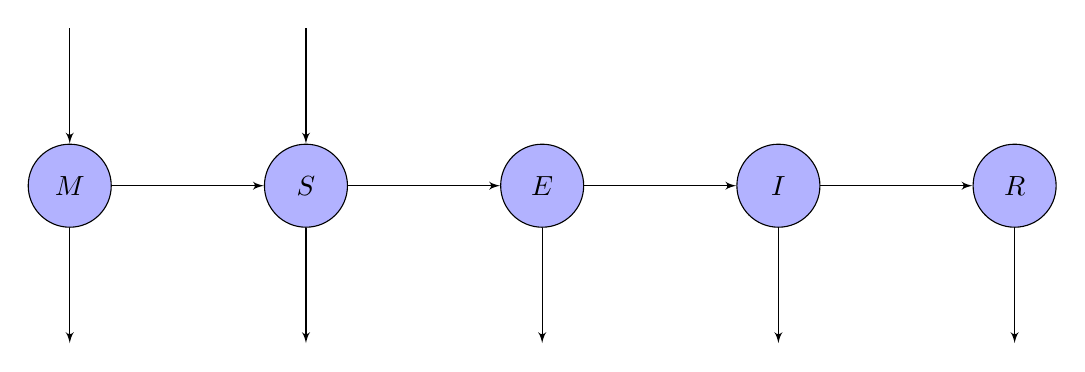
\begin{tikzpicture}[node distance=3cm,auto,>=latex',every node/.append style={align=center}]
  \node [int,  fill = white!70!blue] (s)              {$S$};
  \node[int, fill = white!70!blue] (m) [left of=s] {$M$};
  \node [int,  fill = white!70!blue] (e) [right of=s]             {$E$};
  \node [int,  fill = white!70!blue]           (i) [right of=e] {$I$};
  \node [int,  fill = white!70!blue] (r) [right of=i] {$R$};
  \path[->, auto=false] (s) edge node {} (e)
  (e) edge node {} (i)
  (i) edge node {} (r)
  (m) edge node {} (s)
  ++ (0,2) edge node {} (m)
  (s) ++ (0,2) edge node {} (s);
  \path[->]   (m) edge node {}  ++ (0,-2);
  \path[->]   (s) edge node {}  ++ (0,-2);
  \path[->]   (e) edge node {}  ++ (0,-2);
  \path[->]   (i) edge node {}  ++ (0,-2);
  \path[->]   (r) edge node {}  ++ (0,-2);
\end{tikzpicture}
\caption{Depiction of a MSEIR model with birth and death rates.  $M$ - passive immunity from mother; $S$ - susceptible; $E$- exposed, latent; $I$- infected; $R$ - recovered.  An arrow out of the system indicates death and an arrow into the system indicates birth.}\label{fig::mseir}
\end{figure}


This compartment model approach includes not only the exposed, latent compartment $E$ but additionally the compartment $M$ which stands for passive immunity inherited from the mother.  \cite{hethcote2000} describes the model with the following set of ODES that include birth rate $b$ and death rate $d$, respectively (reparametrized to match our notation),
\begin{align*}
  \frac{dM}{dt} &= b(N-X) - (\delta + d) M \\
  \frac{dX}{dt} &= bX + \delta M - \frac{\beta XY}{N} - dX\\
  \frac{dE}{dt} &= \frac{\beta XY}{N} - (\alpha + d) E\\ 
  \frac{dY}{dt} &= \alpha E - (\gamma + d) Y \\
  \frac{dZ}{dt} &= \gamma Y - dZ \\
  \frac{dN}{dt} &= (b-d)N,
\end{align*}
where $\delta$ is the rate of passive, immune infants transitioning to susceptible indnividuals, $\beta$ is the rate of infection, $\alpha$ is the rate of of infectious individuals becoming infected, and $\gamma$ is the rate of recovery.  The reproduction number is then,
\begin{align}\label{eq:r0-mseir}
\rr &= \frac{ \beta \alpha}{ (\gamma + b)(\alpha + b)}.
\end{align}
\cite{hethcote2000} note that this calculation of $\rr$ may be strictly derived through interpretation of the definition, as ``$\rr$ is the product of the contact rate $\beta$ per unit time, the average infectious period adjusted for population growth of $\frac{1}{\gamma + b}$ and the fraction $\frac{\alpha}{\alpha + b}$ of exposed people surviving the latent class $E$.''  They note that this model is well suited for diseases such as measles, rubella, or mumps where the mother may pass some antibodies to her newborn.  This expression may also be derived using the next generation operator described in Section \ref{sec:ngm}.

Again, this is simply a model for transmission of a disease and does not specify how $\rr$ is to be estimated once the model is written down.  Method such as least squares and MLE are common ways to estimate the parameters in this model and hence $\rr$.  When the birth rate $b=0$, note that $\rr$ reduces to the derived expression for both the SIR and SEIR models without birth and death rates, $\frac{\beta}{\gamma}$.




\subsubsection{Amplifier Model (AMP)}
As mentioned previously, compartment models may be arbitrarily complex.  We demonstrate this idea with a set of compartments for each strain of a disease like influenza or HIV.  \cite{blower2004} discuss the case where a disease may have different strains and consequently a different reproduction number for each strain.  They introduce a multistrain mathematical model called the amplifier model to deal with this case.

This model is based on the the SEIR compartment model, accounting for a number of strains simultaneously.  There is a set of ODEs for each strain of the disease with different parameters for recovery, transmission rate, and drug resistance of the disease.  Additionally, there is mixing of the different strains as ``the amplifier model also allows for immigrating and emigration of individuals of all types, as well as reinfection of latently infected individuals'' \citep{blower2004}.  Ultimately, their formula for $\rr^{(i)}$ where $i$ stands for the $i$th strain is
\begin{align*}
\rr^{(i)} = X^* \frac{ ( \beta_i^Y + \beta_i^E)\alpha_i + \beta_i^Y d_i^E}{(\alpha_i + d_i^E)(c_i + k_{i,i+1} + d_i^Y)}.
\end{align*}
Here, $X^*$ is the number of susceptibles individuals in the disease-free equilibrium in the absence of immigration or emigration; $\beta_i^E$ and $\beta_i^I$ are strain-specific transmission rates for the latent, and infected classes, respectively; $\alpha_i$ denotes the progression rate from latently infected to disease for strain $i$; $d_i^E$ and $d_i^{Y}$ are death rates for the latent and infected classes, respectively; $c_i$ is the cure rate; and $k_{i, i+1}$ is a parameter associated with the degree of amplification of drug resistance.  They note that ``each reproduction number is the product of average number of secondary infections caused per unit time, the average time a case remains infectious and the probability that an infected individual develops disease.''

In the amplifier model, $\rr$ was derived from using the stability point (disease free equilibrium state in the absence of immigration or emigration) of the system by solving the characteristic polynomial for the eigenvalues.  This derivation is explained in more depth in Section \ref{sec:ngm}.

We describe this model as opposed to other available CMs because it shows not only how complex CMs can become, but also to demonstrate how researchers approach the often controversial assumption of homogeneity.  In this case, we have strain-specific transmission rates, so we are essentially stratifying compartments into different groups, allowing for some heterogeneity.  A disadvantage is the amount of strain-specific data required to estimate all parameters, which may be estimated through the usual methods such as least squares and maximum likelihood estimation.


\subsubsection{Next Generation Model (NGM)}
\label{sec:ngm}

Very complicated models have arisen from stratification of compartments such as one with 26 compartments \citep{pandey2014}.  Thus, there is a need to be able to derive an expression for $\rr$ regardless of the structure of the compartment model.   The Next Generation Model (NGM) is a generalization of any compartment model at the infection-free steady state. This model solves the problem of having an expression for $\rr$ in terms of the epidemiological parameters for a general compartment model.  Originally, introduced by \citep{diekmann1990}, \cite{diekmann2009} posit a recipe to find $\rr$ for a wide class of compartment models, including models we discussed, SIR, SEIR, and MSEIR. We summarize that recipe here. First, define the infected subsystem as ``the equations of the ODE system that describe the production of new infections and changes in state among infected individuals.''  Let $x = (C_1, C_2, \dots, C_m)$ where $C_i$ are the different compartments of the infected subsystem.  The steps to find $\rr$ are as follows:


\begin{enumerate}
\item ``Linearize the infected subsystem of nonlinear ODEs about the infection-free steady state''
\item Decompose the linearized infected subsystem into $(T + \Sigma )x$ where $T$ is a $m\times m$ matrix of transmissions and $\Sigma$ is a $m \times m$ matrix of transitions.
\item $\rr$ is the spectral radius (i.e. the dominant eigenvalue) of $K_L=-T \Sigma^{-1}$.  
\end{enumerate}

Here, $T_{ij}$ is the rate of transmission of \textit{newly} infected individuals in state $i$ created by individuals in state $j$.  $\Sigma_{ij}$ is the transition rate of individuals into compartment $i$ from compartment $j$.

This method has the assumptions of a basic compartment model: homogeneous mixing among populations and the law of mass action, i.e., that the number of infected individuals are proportional to the number of infected individuals at the previous step.   Additionally, this method is advantageous in that the matrix $-\Sigma^{-1}$ has intuitive meaning.  The $ij$th entry of $- \Sigma^{-1}$ is the ``expected time that an individual who presently has state $j$ will spend in infected state $i$.''

Although, this method is useful for deriving an expression for $\rr$, it is unclear how to actually estimate it from these expressions.  One could use maximum likelihood if one specifies distributions for how compartments change over time or least squares may be applied. In general, adding numerous compartments is often tedious and difficult and needlessly complex.  Instead, researchers have started to lean towards ABMs when introducing heterogeneity in their models, which we describe in Section \ref{sec:network}.  

%%%%%%%%%%%%%%%%%%%%%%%%

\subsection{Exponential Growth}\label{sec:exp-growth}
Typically, CMs expressed through ordinary non-linear differential equations have no known analytical solutions, which makes deriving a closed-form expression for $\rr$ difficult or impossible.  One simplification that is often introduced to the SI-framework is that of exponential growth, or that the number of infections in the beginning of an epidemic mimics that of an exponential curve.  This simplified expression has allowed for many derivations of $\rr$.


\subsubsection{Exponential Growth (EG)}
\label{sec:expgrowth}
\cite{wallinga2007generation} report that the effective reproduction number $\mathcal{R}_t$ and hence the initial reproduction number $\rr$ may derived using the fact that infection ``counts increase exponentially in the initial phase of an epidemic.''  We then have to estimate $r$, the \textit{per capita} change in the number of new cases per unit of time and $\omega$ the serial interval, the distribution of time between a primary and secondary infection. Then, we have
\begin{align}\label{eq:lotka}
\rr = \exp{(r \omega)}
\end{align}
or its first order approximation
\begin{align}\label{eq:anderson}
\rr = 1 + r \omega.
\end{align}
Equation \eqref{eq:lotka} is derived from a demographic view using the Lotka-Euler survival equations which come from the fields of demography, ecology, and evolutionary biology, whereas Equation \eqref{eq:anderson} is derived through an epidemiologist's perspective. 

\cite{wallinga2007generation}, instead, use a moment generating function expression for $\rr$.  With $\omega(t)$ as the serial interval, then
\begin{align*}
\rr^{-1} &= \int_{a=0}^\infty e^{-rt}\omega(t)dt.
\end{align*}
For all these above estimates of $\rr$, we observe the duration of serial intervals in a period of exponential growth.  Deciding when exponential growth occurs and which data points to use to estimate $\rr$ is difficult.  \citeauthor{wallinga2007generation} specify $\omega$ in multiple ways.  Parametrically, they use exponential, normal, and point-wise distributions.  Additionally, they discuss using the the empirical distribution of the serial interval.

\citeauthor{wallinga2007generation} note that specifying the epidemic model ``implicitly specifies a generation interval distribution.''  The above equations are under the SIR framework, but this method may be adapted to acommodate other frameworks.

\subsubsection{Maximum Likelihood Estimator of Secondary Infections (MLSI)}\label{sec:mle-si}
A common method used to estimate parameters in the SI-framework is maximum likelihood estimation.  This method requires assuming the likelihood of a parameter given the data observed, and hence many distributions may be specified.  The MLE of secondary infections, described by \cite{forsberg2008}, finds the estimate of $\rr$ by maximizing the likelihood function under a certain assumptions.  We assume that the ``the number of secondary cases produced by an infected individual follows a Poisson distribution, and that the serial interval is described by a multinomial distribution.''  Recall, the serial interval is the distribution of time between a primary case developing symptoms and a case infected by the primary case developing symptoms.  An approximate version of this can be simplified to a thinned Poisson  where
\begin{align}\label{eq:mlesi}
  L(\rr, \mathbf{p}) = \prod_{t=1}^T \frac{e^{- \rr \sum_{j=1}^{\min(k,t)}J_{t-j}p_j}\left (\rr \sum_{j=1}^{\min(k,t)}J_{t-j}p_j \right )^{J_t}}{J_t!}.
\end{align}
Here, $k$ is the maximal amount of the serial number (the maximum amount of time between infections), $T$ is the total time and $p_j$ is the probability of displaying symptoms on day $j$ after being infected.  The number of cases on day $t$, $J_t$ are observed incidence counts.

This method assumes that the number of new cases caused by an infected individual follows a Poisson distribution with mean $\rr$ and that hte serial interval follows a multinomial distribution. Additionally, this method also assumes a period of exponential growth.  An advantage of this specification is that we can write down a nice likelihood for $\rr$. Two disadvantages are that we only have an approximation for $\rr$ and have to decide which data points to use in a certain time frame.  Additionally, we have to validate our assumptions about the specified distributions.  This method was used to estimate $\rr$ for Ebola, Avian Influenza, and Swine Flu.


%%%%%%%%%%%%% 5

\subsubsection{Time Dependent Reproduction Number (TDR)}\label{sec:timedep}
Another likelihood based approach to estimate $\rr$ is that of the time dependent reproduction number, as shown by \cite{wallinga2007generation} and summarized by \cite{obadia2012r0}.  They maximize the likelihood that case $i$ has been infected by case $j$ at certain time using the serial interval, $w(t)$ where $t_i$ is when case $i$ was infected and $N$ is the total number of cases,
\begin{align*}
  p_{ij} &= w(t_i- t_j) / \sum_{i \neq k} w(t_i - t_k),\\
  \rr &= \frac{1}{Y(0)}\sum_{i=1}^N p_{i0}
  \end{align*}
  A disadvantage of this method is that it assumed we have knowledge about the serial interval distribution, $w(t)$, but an advantage is that the method works with any specification of $\omega$.  This method also requires that the initial number of susceptibles $X(0)$ is roughly the size of the total population.  Another advantage is the explicit use of distributions to indicate that $\rr$ is indeed a random variable.  This method was used to estimate $\rr$ for Influenza A.

\subsubsection{Initial Growth Rate and Final Size (IGRFS)}
\label{sec:igr-fs}

Initial growth rate, as described by \cite{dietz1993estimation} is derived by \cite{anderson1986}, initially to study the spread of HIV.  Initial growth rate estimates $\rr$ through
\begin{align*}
\rr = \frac{D \ln 2} {t_d} + 1,
  \end{align*}
  with $D$ as the average incubation period and $t_d$ as the doubling time during its early stages.  This method assumes one knows when the ``early stage'' ends along with knowledge of the average incubation period.  

  Final size, on the other hand, only looks at $\rr$ once a disease has run its course.  Here $\mu_0$ is the proportion of initially infected individuals and $\mu_\infty$ is the final, cumulative proportion of infected cases at the end of an epidemic,
\begin{align}\label{r0_attackrate}
\rr =  \frac{\log \left ( \frac{X(0)}{\mu_{\infty} N}\right )}{\mu_\infty - \frac{X(0)}{N}}
\end{align}
This method can only be used to assess $\rr$ after a disease has passed through a population.  Additionally, if either $\beta$ or $\gamma$ were affected during the disease's lifetime, such as through interventions and prevention strategies, then $\rr$ cannot be properly assessed.

  These two methods allow one to look at $\rr$ at both the beginning and the end of an epidemic.   For the initial growth rate, while one can see $\rr$ at early stages, estimating the doubling time $t_d$ is difficult.  For final size, one has to wait until the end of an epidemic to calculate $\rr$, and prevention strategies may skew the final result.  These methods were used to estimate $\rr$ for AIDS and smallpox.
%%%%%%%%%%%%%%%%%%%%%%%%%%%%%%

  \subsection{Estimation from Networks}
As estimating $\rr$ is concerned with the number of new infections based on the contacts of old infections, a network is a seemingly intuitive way to model such contacts and hence infections.  Networks that have been used to estimate $\rr$ include contact tracing of actual individuals, branching processes to model the spread of disease, and agent-based models (also known as individual level models), which all leverage networks along with different sources of data to generate estimates of $\rr$.  Additionally, networks provide an intuitive framework in which individuals can interact with varying levels of heterogeneity.  However, when using a network approach, we must be careful of our interpretation of $\rr$ as we often are conditioning on certain individuals.    \cite{breban2007} note that calculating $\rr$ from a network approach may give misleading results due to conditioning on the network structure.
  
\label{sec:network}

%%%%%%%% 5
\subsubsection{Contact Tracing (CT)}
\label{sec:contact_tracing}
A reasonable idea to estimate $\rr$ is to directly observe the number of secondary infections produced by an initial infector.  However, this approach is generally impractical as it is difficult to estimate every single contact an individual may have.   With seriological information, we could conceivably recreate the transmission of the disease throughout a population.  Even in this case it is unlikely, for one, to have a completely susceptible population, which is essential to an unbiased estimate of $\rr$.  Moreover, this would implicitly be conditioning on the initial infector's contacts which may not reflect those of the rest of the population.  We write the calculation for $\rr$ under contact tracing in Equation \ref{eq:r0_contacttracing}, where $X_0$ is a random variable denoting the number of individuals in the population individual 0 infects.  Here $X(0)=N$ indicates that the initial number of susceptibles is $N$, the size of the population,
\begin{align}\label{eq:r0_contacttracing}
\rr = E[ X_0 | X(0) = N].
\end{align}
\cite{eames2003} describe contact tracing as an ``extreme form of targeted control, where the potential next-generation cases are the primary focus.'' That is, one focuses on treating the contacts of an infected individual rather than applying uniform treatment across a population.

They describe an estimate for $\rr$ for a SIR model on a network, with $r$ as the rate of transmission across a contact multiplied by the infectious period and $n$ as the number of contacts as
\begin{align*}
\rr = r(n-2)
\end{align*}
Again, the difficulties of this method lies in one, estimating the contacts of an initial infected individual and two, extrapolating the contacts of the initial individual to the population as a whole.  As such, although important in treating an outbreak of a disease in its early stages, is not the best choice to estimate $\rr$ due to the high level of uncertainty inherit in the method and due to conditional assumptions of the initially infected individual.


%%%%%%%%%%%%%%%%%%%%%%%%%%%%%%%%

\subsubsection{Branching Process (BP)}
\label{sec:branching-process}

Branching processes are models for population growth which track generations of new offspring.  We describe branching processes as adapted for epidemic modelling from \cite{grimmett1992}.  An infector $i$ may produce new infections, called offspring, over the duration of the  infector $i$'s disease.  The offspring of the original infector directly produces are called the first generation.  The offspring of the first generation are called the second generation and so on.  This process is illustrated in Figure \ref{fig:bp}.  An important assumption in branching processes is that the offspring produced from different infectors are indepedent and identically distributed, and so for a branching process to be a valid model in epidemic modeling, we must assume a large population with few infectors.

\begin{figure}
  \centering
\begin{tikzpicture}
  [
    grow                    = right,
    sibling distance        = 4em,
    level distance          = 10em,
    edge from parent/.style = {draw, -latex},
    every node/.style       = {font=\footnotesize},
    sloped
  ]
  \node {Case 0}
  child { node {Gen. 1}
    child {node{ $\dots$}}
  }
  child {node {Gen. 1}
    child{ node  {$\dots$}}
  }
  child{ node  {Gen. 1 }
    child{ node  {Gen. 2}
    }
    child{ node {Gen 2}
      child{ node  {$\vdots$}}
      child{ node  {$\vdots$}}
      child{ node  {$\vdots$}}}
  };
\end{tikzpicture}
\caption{Illustration of a branching process.}\label{fig:bp}
\end{figure}

\cite{getz2006} give a way to calculate $\rr$ from a branching process.  ``We define the offspring distribution $\{q_i \}_{i=0}^\infty$, where $q_i$  is the probability that an infectious individual infects $i$ other individuals.  Thus we require $\sum_{i=0}^\infty q_i =1$ and note that $\rr$, the mean number of cases contracting disease from each infective'', is simply given by'
  \begin{align*}
    \rr = \sum_{i=0}^\infty iq_i.
  \end{align*}
  It is assumed we know how to estimate the $q_i$, and so in this case, it is not too different of an approach than contact tracing.  The disadvantages of this method are similar to that of contact tracing as data about which individuals  infected another is very difficult to obtain.  An advantage is that this method directly gets to the ``heart'' of the definition of $\rr$ as it is concerned with generations of infected individuals rather than incidence at a certain time.


    

\subsubsection{Agent-Based Models (ABM)}
\label{sec:agent-based-models}
Agent-based models (ABMs) or individual level models (ILMs) are ``bottom-up'' models, meaning micro patterns are simulated and macro patterns are then inferred from these micro patterns.  ABMs consist of agents which represent individuals (e.g., people, mosquitoes, poultry) and a series of activities in which the agents can affect one another and evolve over time.

In epidemiology, ABMs may be used to simulate the spread of disease.  ABMs allow for every detail of an infection to be known, in the context of estimating $\rr$, meaning we know exactly who is infected by whom and when.  Let $L$ be the number of simulations run and $X_{n \ell}$ be the number of infections caused by agent $n = 1, 2, \dots, N$ who was infected at time $t=0$ in simulation $\ell$.   Thus $\rr$ can be estimated simply through
\begin{align*}
  \rr =& \frac{1}{LN}\sum_{\ell =1}^L\sum_{n=1}^NX_{n \ell}
\end{align*}
Examples of estimations of $\rr$ using ABMs/ILMs are in \cite{breban2007,ahmed2013variance}.

There are many advantages to using ABMs, a main one being able to run the model multiple times under the same initial conditions.  In this way, one can easily obtain variance estimates of $\rr$ in addition to empirical distributions of it.  Moreover, this estimation can accommodate any model specification of how the disease is transmitted through the population.  However, the major disadvantage of the ABM lies in calibrating the evolving of agents over time to accurately reflect reality, a problem that cannot be understated.  Thus, it is typically necessary to have knowledge of parameters such as the serial interval, transmission rate, recovery rate, etc.  Additionally, we need to have accurate agents in characteristics and their implied network structure.  ABMs are flexible in that they may be used with any model in the SI framework.  The only requirement is that we track who infects whom and can adapt for any additional states such as exposure or prevention strategies such as closing schools \citep{fred}.







\subsection{Variance Methods}
\label{sec:methods}

Estimating $\rr$ is difficult and estimating $V[\rr]$, the variance, is even more so.  We describe general methods which may be applicable to estimate the variance.  We describe the assumptions that are used along with each method and note that they may not be applicable to all of our methods.  Still, reporting confidence intervals is very important, and we hope to encourage this practice by describing the below methods used to estimate models in the SIR framework in a simple fashion.  Regardless of the method used to estimate variance, confidence intervals, or credible intervals, we encourage researchers to carefully examine all underlying assumptions of 1) specifying a model for disease transmission, 2) estimating $\rr$ from the model, and 3) the method used to estimate the variance or CIs.


\subsubsection{Delta Method}\label{delta-method}

When the method estimates \(\beta\) and \(\gamma\) instead of \(\rr\) directly, we use the delta method approximation to calculate the
variance of \(\rr\). Here, we know \(\rr = h(\beta, \gamma) = \frac{\beta}{\gamma}\). Then \(\bigtriangleup h = (\frac{1}{\gamma},  -\frac{\beta}{\gamma^2})^T\) and \(V[\rr] = \bigtriangleup h^T \Sigma_{\beta, \gamma} \bigtriangleup h\), where \(\Sigma_{\beta, \gamma}\) is covariance matrix of \(\beta\) and \(\gamma\).

This estimate assumes that the distribution of $\beta$ and $\gamma$ are asymptotically normal.  Here, we use the relationship of $\rr = \frac{\beta}{\gamma}$ in order to estimate the variance, which is specific to the SIR framework.  This method may be extended to other frameworks.  The advantages of the delta method are that as the NGM posits a recipe to derive $\rr$, then it is theoretically possible to use the delta method to derive an expression for the variance of $\rr$ for any compartment model.


\subsubsection{Posterior Distribution}
When one uses a Bayesian approach to estimate $\rr$, the result should be a distribution rather than an estimate.  One can simply look at the quantities of this distribution to form a credible interval for this estimate.  Advantages of this method include having an entire distribution compared to a point estimate.  One disadvantage is that the Bayesian approach will not guarantee frequentist properties that epidemiologists may be looking for such as being able to compare diseases to one another.



%%%%%%%%%%%%%%%




\section{Analysis and Results}
\label{sec:results}

\subsection{Comparing Models}

\textit{We compare the different ways to estimate $\rr$ to see which ones give more accurate and reliable estimates.}  As there is no way to know the ``true'' $\rr$ of an actual disease we compare our methods by fitting them to simulated data sets and look at the resulting $\rr$ estimates and standard errors. Our main comparisons are done with data generated from the SIR model with random error added so that we can compare model estimates to a known true $\rr$ value. We vary the conditions under which the SIR data is generated to see how the results from the estimators change. We also look at data from different functional models to see how the estimators perform under different circumstances.

%% What do you mean by describing the standard standard deviations?
%% SG: delta_t is normally distributed with sd sigma and similarly for other methods.  How and why did we pick the numbers that we did?



\subsubsection{SIR Data}

\textit{The datasets from the SIR model are simulated from the ODEs: \begin{align}
	\systeme{\frac{dX}{dt} = -\frac{\beta XY}{N}, \frac{dY}{dt} = \frac{\beta XY}{N} - \gamma Y, \frac{dZ}{dt} = \gamma Z}.
	\end{align}
} 

We use arbitrarily selected the parameters to generate the time series data set from the SIR model. We first generate "baseline" data from which we can make comparisons by changing the  conditions under which the data were generated. The baseline SIR data are simulated with the following conditions:

\begin{center}
	
	$\beta$ = 0.006, $\gamma$ = 0.003; $\rr$ = 2
	
	Number of time steps: 365
	
	Starting X size ($X_0$): 99950
	
	Starting Y size ($Y_0$): 50
	
	Starting Z size: 0
	
	Total population: 100000.
	
\end{center}

%% Is this enough detail on describing the initial S, I, and R, or are we looking for something more specific?

\textbf{Our baseline initial size for $Y_0$ is 0.05\% of the total population in our simulated environment, which is fairly large compared to the starting point for the data in most epidemics. However, I/we felt that this was necessary in order to see the differences between the models.}

We then generate random errors that are added to the X and Y compartments at each time step in order to simulate some form of randomness. \textbf{The sum of these was then subtracted from the Z compartment in order to keep the total population in the system constant.} We generated data sets with two different types of errors: Gaussian and autoregressive. \textbf{The Gaussian errors are independently distributed with mean 0 and constant variance for the entire length of the time series. The autoregressive errors are generated from a first-order process of the form: $$ \epsilon_{t} = \rho * \epsilon_{t-1} + \delta_{t}$$, where $\rho$ is fixed throughout and $\delta_{t} \sim N(0, \sigma)$ with constant $\sigma$. The values of the variances are chosen somewhat arbitrarily, although they are intended to be fairly small at first.} 

We also add a monotonicity adjustment to the X and Z compartments with both of the error models. \textbf{This is done using the Pool Adjacent Violators Algorithm (PAVA); the algorithm checks if the observation at each time step is greater than or equal to the previous one, and changes the value of both observations to be equal to the mean of the two if the condition is not fulfilled.} This gives us a total of four error models: autoregressive (Auto), autoregressive monotonic (AutoM), Gaussian (Norm), and Gaussian monotonic (NormM). For our baseline data, we have ($\sigma_X, \sigma_Y$) = (10, 1). We simulate 5 different baseline sets to see how consistent each of the models are.

\textit{To see the effects of different conditions for the data, we change one of the starting conditions while holding all of the other ones constant. We try changing two conditions: the starting number of susceptible and infected people in the population (holding the total population constant) and the variance of the errors added on to the The starting population sizes for the $X$ and $Y$ are set to ($X_0$, $Y_0$) =  (99999, 1), (99990, 10), (99900, 100), and (99000, 1000), holding all other conditions constant. The variance of the added errors by scaling them to: ($\sigma_X$, $\sigma_Y$) = (10, 1), (100, 10), (500, 50), (1000, 100), (2000, 200), (5000, 500), (10000, 1000), (15000, 1500); these are done with ($X_0$, $Y_0$) = (99000, 1000). The errors start very small but become very large relative to the actual compartment sizes; this allows us to more clearly see the effects of the changes.}

%% Describe the initial S, I, R values
%% Describe the different error methods
%% Describe the standard standard deviations involved
%% High level fitting comments

%% Throw fitting details into the appendix

%% Talk about top 3-5 methods
%%%%%% Honestly, all the methods seem to have flaws in one way or another - maybe point out why?
%% Talk about methods that really miss
%% Talk about the standard error reports
%% Talk about 4 categories.  Does anyone do worse/better?
%% What about the one where we cannot estimate std
%% What happens when SD is large?


%% Throw some graphs in


\subsubsection{Other Models}
We simulated data from 6 other models besides the classic SIR model. 5 of these were polynomial linear regression models, from order 0 to 4 with respect to time/day. The coefficients used to generate data from the linear regression models were originally chosen by taking the approximate coefficient estimates from fitting the linear regression models to classic SIR data. This does not necessarily guarantee that the true $\rr$ will be 1.2, especially for the 0th and 1st order linear regression models. What we are interested in for these cases is to see if the models still give reasonable estimates for $\rr$. The other model is the linear SIR model, which is a three compartment model with the following ODEs:

	\begin{eqnarray*}
		\frac{dS}{dt} &=& -\beta I \\
		\frac{dI}{dt} &=& \beta I - \gamma I \\
		\frac{dR}{dt} &=& \gamma I.
	\end{eqnarray*}

 The data from the linear SIR model were simulated with parameters $\beta$ = 0.06 and $\gamma$ = 0.05, such that $\rr$ = 1.2. This model will allow us to compare how the SIR models perform under misspecified differential equations.
 
 \textbf{Random error is added to the data generated here as well using the same 4 error models as above. The other specifications for these datasets are the same as for the baseline classic SIR data, namely the variance of the added errors and starting compartment sizes.}

\subsubsection{Variance Estimation}

\textbf{The method for calculating the standard errors for $\hat{\rr}$ depend on the model used. The following models take the standard error directly from the regression methods used to estimate $\rr$:}

	\begin{itemize}
		\item SIR LMA
		\item SIR LMAT
		\item SIR Log Linear
		\item SIR MC
		\item Exponential Growth
		\item Initial Growth
	\end{itemize}

\textbf{The ones that are calculated using the delta method:}
	
	\begin{itemize}
		\item-SIR LS
		\item SIR ReLS
		\item SEIR
		\item MSEIR
		%% \item AMP
		\item NGM
		\item Final Size
	\end{itemize}
	

Standard errors for the maximum likelihood and branching process models are calculated using the negative reciprocal of the Fisher information. The sequential Bayes model uses the standard deviation from the posterior distribution. We use the jackknife method to estimate the standard error of the SIR smoothed max and the SIR smoothed IPR methods. The jackknife calculates the standard error using the standard deviation of estimates of $\rr$ after leaving out a single data point.
	
Some of the models use only one single point in time to estimate $\rr$ and therefore do not seem to have an innate source of variance. We currently do not have standard errors for the SIR Max and SIR IPR models.

\subsection{Results}

\subsubsection{Survival Function}

\textbf{STILL NEED TO ACTUALLY DO DPE}

We do not have a direct way to estimate $/rr$ using the survival function method from the data we have. The method requires a density estimate of the survival function at each point in time. Either we would need to have some prior knowledge or assumptions about what the survival function for a particular disease was, or we would need to search over a space of possible function and possible parameter values to estimate $/rr$. For similar reasons, we can not estimate $/rr$ using the Von Forester equations using the data we have, as we would need to know the infectivity of a diseased individual over time. This may be possible for a known, well studied disease, but may not be  For the direct parameter estimation method, assuming the population is homogeneous and that we know the average duration of infection, we can estimate the probability of transmission parameter and its standard error by averaging over the ratio between percent change in the susceptible compartment and the prevalence of the disease at each time step.



\subsubsection{Compartment Models}

\paragraph{SIR Models}
%In general, the models derived from the SIR ordinary differential equations are relatively accurate. Most estimates are within the range of $\pm$ 0.2 of the true $\rr$ for the baseline SIR datasets. The magnitude of the standard errors on the baseline datasets for the different SIR models generally depend on the method used. The models that estimate $\rr$ using optimization or gradient descent, namely SIR LS and SIR ReLS, have standard errors on the order of $10^{-4}$ to $10^{-7}$. The standard errors are somewhat larger for the methods that use regression, on the order of $10^{-1}$ to $10^{-3}$. 

%The SIR models as a whole also do fairly well with changing the starting number of infected people. However, they tend not to do as well when the variance of the added errors is very large; in these situations, many of the models tend to have very large standard errors, sometimes on the order of $10^{1}$ or $10^{2}$.

%The exceptions to the above are the linear, incidence-prevalence ratio, and Markov chain models. The estimates tend to be far from the true $\rr$, and they fluctuate greatly between the baseline data sets. The standard errors for these models (if they exist) also tend to be very large under some of the changing conditions.

%Many of the SIR models do not work as well with the data that come from the polynomial linear models. Specifically, for the 0th and 1st order model datasets, the estimates can be unreasonably large or negative. The Log linear, Sequential Bayes, Smoothed max, and Max models do not have this problem. 

\paragraph{Other Compartment Models}

%All of these models use optimization to estimate the parameters that are used to calculate $\rr$. They tend to be fairly accurate and consistent on the baseline data, often as good as or better than those from the various SIR models. The SEIR models (least squares and next generation) do not handle the large added errors very well, as it tends to give ridiculously large results. The standard errors tend to be on the order of $10^{-2}$ to $10^{-3}$. However, as with the estimates above, the standard errors from the SEIR models can become unreasonably large when the variance of the added errors becomes large. Also, as with the SIR models, the $\rr$ estimates and standard errors from the 0th and 1st order polynomial linear model datasets are not very good, as the former is sometimes negative and the latter can be very large. The MSEIR model tends to do fairly well in all situations.

\subsubsection{Exponential Growth}

%We have assumed for these models that the number of infections follows an exponential curve throughout the entire time frame of the data sets. This assumption certainly does not hold for the data from the 0th and 1st order linear models, and may not hold for some of the other data sets either. 

%These models are generally not as accurate as the compartment models above. Most of them, except for the initial size model, tend to underestimate $\rr$, with estimates between 0.8 and 1.0. The standard errors are all fairly small, on the order of magnitude from $10^{-1}$ to $10^{-3}$. This is larger than many of the compartment model standard errors. The main advantage that all of these models, except for the maximum likelihood model, seem to be more robust to changing conditions and functional forms of the data compared to the compartment models. The estimates and standard errors for $\rr$ appear to be reasonable in all cases, including for very large added errors and for the 0th and 1st order linear model data.

\subsubsection{Network Models}

%The branching process model (the only one in this category so far) is not very accurate. In particular, for the SIR datasets, the $\rr$ estimates are less than 1, while the true $\rr$ is greater than 1. The standard errors, though, are relatively small, around the same order of magnitude as the SIR least squares models. Model estimates and standard errors are fairly consistent across the baseline datasets and changing starting compartment sizes. However, increasing the standard deviation of the added errors tends to have a somewhat noticeable impact on model results. The model also does not handle the 0th order polynomial linear data well.


\section{Discussion}
\label{sec:dis}

Below, we compare the estimates and standard errors of $\rr$ given by each of the models for a few selected data sets using forest plots; they show the point estimates and 95\% confidence intervals of $\rr$ from each model for a particular data set. The true $\rr$ value is also shown by the vertical red line in the graphs. All of the figures below show results from data sets that were simulated with added Gaussian errors. The plot on the top left shows the estimates from one of the baseline data sets. For the most part, the $\rr$ values range from approximately 0.8 to 2. We note that many of the models estimate an $/rr$ value of approximately 1, and some estimate that $/rr$ is less than 1. This would indicate that the infection disease is growing very slowly or is actually dying out, when in reality the disease is spreading at a fairly rapid rate. The confidence intervals are very small relative to the estimates for the most part; exceptions to this include the SIR IPR and LMA models as well as the Markov chain model. 

The plot on the top right shows the estimates for the data set where $Y_0$ is increased to 1000. The $\rr$ estimates are almost all further away from the true $\rr$ value compared to the results from the baseline data sets. The confidence intervals are also more often than not larger than those in the baseline. In particular, the standard errors for some of the SIR models increase by several orders of magnitude.

The bottom left plot shows the estimates for the data set where the error added to the generated data is increased. For most of the models, the estimates of $\rr$ decrease slightly, and overall they do not change very much compared to the baseline data set. The confidence intervals for this data set increase substantially for some models, such as the SIR LMA, while they remain approximately the same as the baseline data sets for several of the others.

On the bottom right, we see the $\rr$ estimates for the case when disease prevalence grows linearly, as opposed to exponentially as seen in the data sets generated under SIR conditions, where the disease prevalence grows exponentially. Model performance here varies depending on how well the models the aforementioned linear growth. Some of the models, such as the SIR Markov chain and the IPR models, do not handle this case very well, giving much larger estimates and standard errors than are reasonable. On the other hand, models such as the SIR maximum and final size seem to be more flexible to different trajectories.

\begin{minipage}{0.5\linewidth}
	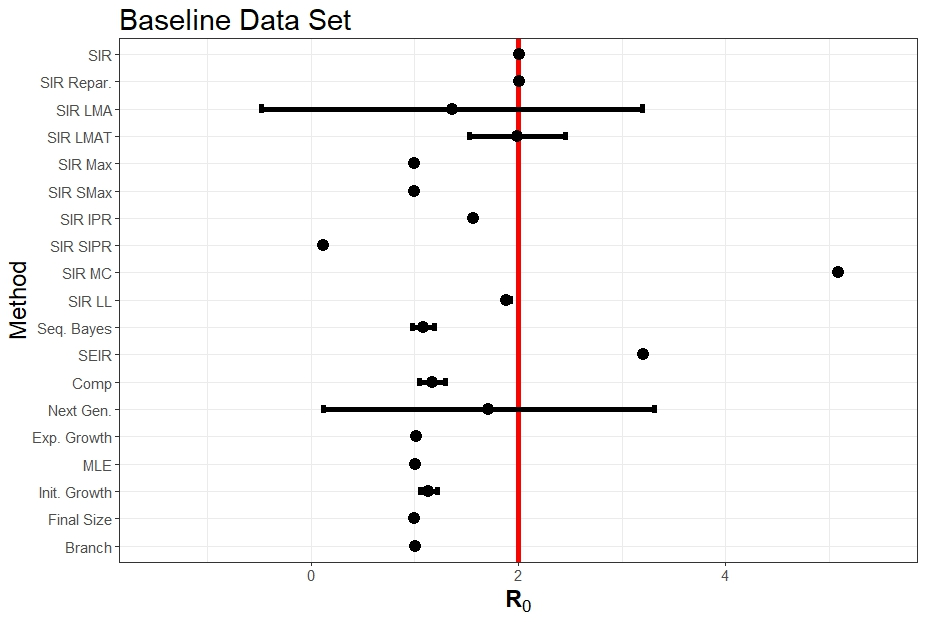
\includegraphics[width=3in]{BaselineFP.jpeg}
\end{minipage}
\begin{minipage}{0.5\linewidth}
	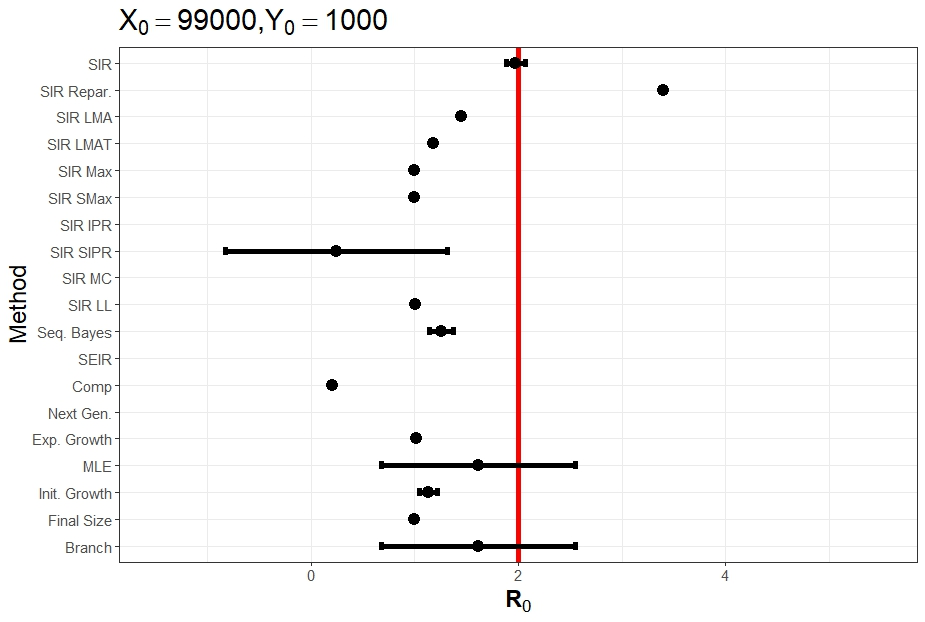
\includegraphics[width=3in]{StartPopFP.jpeg}
\end{minipage}


\begin{minipage}{0.5\linewidth}
	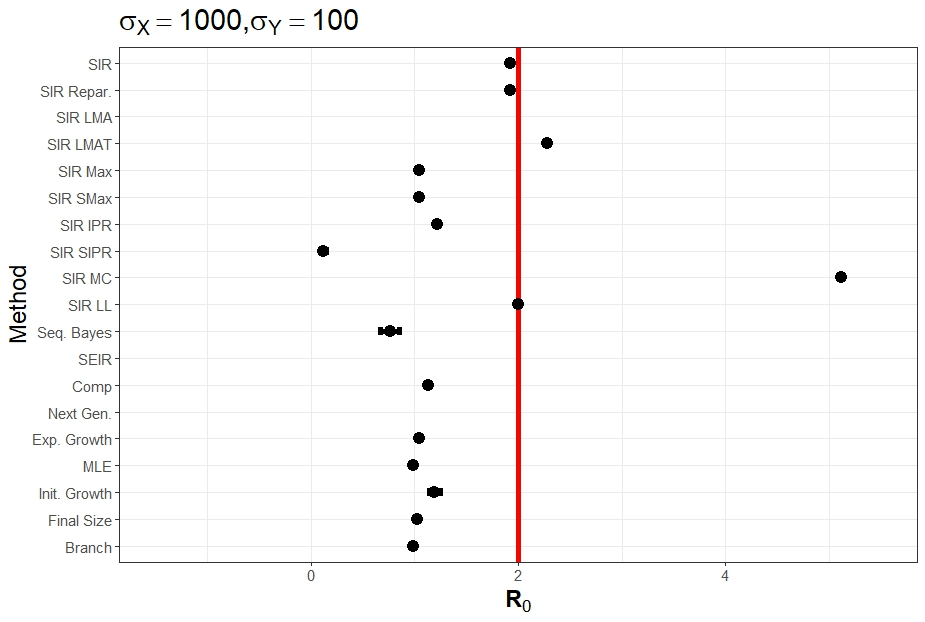
\includegraphics[width=3in]{VarianceFP.jpeg}
\end{minipage}
\begin{minipage}{0.5\linewidth}
	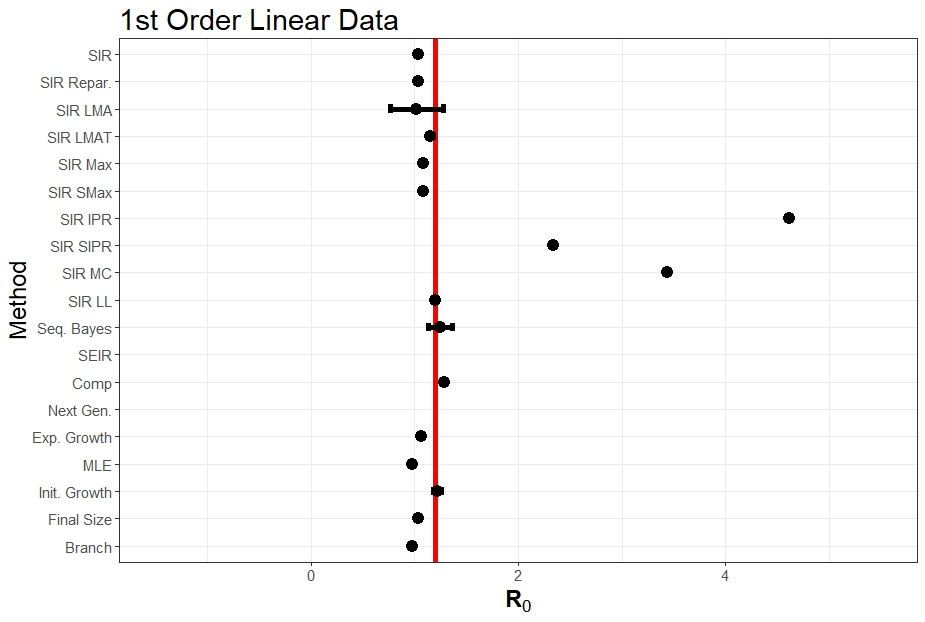
\includegraphics[width=3in]{OtherFP.jpeg}
\end{minipage}

\bibliographystyle{apa}%Choose a bibliograhpic style
\bibliography{Master}


\section{Appendix}

Included here are the technical details for fitting the models in R, as well as tables of the results.

\subsection{Compartment Models}

\subsubsection{SIR Least Squares}

\paragraph{Estimation}

For the least-squares SIR model, we estimate the parameters $\beta$ and $\gamma$ of the ODEs using optim() in R to minimize the sum of squared errors using Nelder-Mead. The standard errors for $\beta$ and $\gamma$ were estimated using the Hessian matrix given to us by optim(), and then the standard error for $\rr$ was calculated using the delta method.

\paragraph{Comments}

The $\rr$ estimates for the baseline data are both close to the actual value, and the standard errors were relatively small. We would probably expect this given that this is the same model from which the data were generated. 

For the changing compartment sizes, we see that the standard errors are much larger for smaller values of $Y_0$. This might be because the variance of the I compartment is much larger relative to the size of the compartment, since we hold $\sigma_Y$ at 1 no matter if $Y_0$ is 1 or 1000. 

For the changing error variances, we see that the estimates for $\rr$ become less accurate for increasing $\sigma_X$ and $\sigma_Y$. However, it is interesting to note that the standard errors are increasing for the monotonic Gaussian error data, but decreasing for the autoregressive and monotonic autoregressive error data and relatively stable for the Gaussian non-monotonic data. It is not clear why this would be the case.


\begin{table}[H]
	\caption{$\rr$ Estimates and Std. Errs, SIR Model, 
		Baseline Data, $X_0 = 99950, Y_0 = 50$, 
		$\sigma_X = 10, \sigma_Y = 1$}
	\begin{footnotesize}
		\hskip -1cm
		\begin{tabular}{l|r|r|r|r|r|r|r|r}
			\hline
			Data Set & Auto Est & Auto SE & AutoM Est & AutoM SE & Norm Est & Norm SE & NormM Est & NormM SE\\
			\hline
			Baseline 1 & 1.965322 & 0.000869 & 1.983308 & 0.000882 & 2.005867 & 0.000893 & 1.994736 & 0.000884\\
			\hline
			Baseline 2 & 2.039608 & 0.000913 & 1.999245 & 0.000895 & 2.001217 & 0.000889 & 1.995960 & 0.000887\\
			\hline
			Baseline 3 & 2.005609 & 0.000901 & 1.966631 & 0.000873 & 2.016216 & 0.000901 & 1.997175 & 0.000887\\
			\hline
			Baseline 4 & 1.958037 & 0.000859 & 1.941109 & 0.000852 & 1.995544 & 0.000886 & 2.004107 & 0.000892\\
			\hline
			Baseline 5 & 2.050904 & 0.000926 & 1.964328 & 0.000866 & 2.009912 & 0.000896 & 1.990153 & 0.000881\\
			\hline
		\end{tabular}
	\end{footnotesize}
\end{table}


\begin{table}[H]
	
	\caption{$\rr$ Estimates and Std. Errs, SIR Model,
		Different Starting Populations, 
		$\sigma_X = 10, \sigma_Y = 1$}
	\begin{footnotesize}
		\hskip -1.7cm
		\begin{tabular}{l|r|r|r|r|r|r|r|r}
			\hline
			Data Set & Auto Est & Auto SE & AutoM Est & AutoM SE & Norm Est & Norm SE & NormM Est & NormM SE\\
			\hline
			$X_0 = 99999, Y_0 = 1$ & 1.689292 & 0.020794 & -4.167216 & 0.168853 & 1.976254 & 0.045081 & 1.688593 & 0.029680\\
			\hline
			$X_0 = 99990, Y_0 = 10$ & 2.038297 & 0.004597 & 2.207003 & 0.005165 & 2.037726 & 0.004596 & 1.883084 & 0.004049\\
			\hline
			$X_0 = 99900, Y_0 = 100$ & 2.009581 & 0.000449 & 2.006557 & 0.000448 & 1.999236 & 0.000445 & 1.995467 & 0.000444\\
			\hline
			$X_0 = 99000, Y_0 = 1000$ & 2.002521 & 0.000046 & 2.001829 & 0.000046 & 1.999519 & 0.000046 & 2.000098 & 0.000046\\
			\hline
		\end{tabular}
	\end{footnotesize}
\end{table}

\begin{table}[H]
	
	\caption{$\rr$ Estimates and Std. Errs, SIR Model, 
		Different Variances, $X_0 = 99000$, $Y_0 = 1000$}
	\begin{footnotesize}
		\hskip -1.7cm
		\begin{tabular}{l|r|r|r|r|r|r|r|r}
			\hline
			Data Set & Auto Est & Auto SE & AutoM Est & AutoM SE & Norm Est & Norm SE & NormM Est & NormM SE\\
			\hline
			$\sigma_X = 10, \sigma_Y = 1$ & 1.927444 & 0.000059 & 1.927090 & 5.9e-05 & 1.925768 & 5.9e-05 & 1.926576 & 5.9e-05\\
			\hline
			$\sigma_X = 100, \sigma_Y = 10$ & 1.926786 & 0.000058 & 1.916571 & 5.9e-05 & 1.919778 & 5.9e-05 & 1.929422 & 5.9e-05\\
			\hline
			$\sigma_X = 300, \sigma_Y = 30$ & 1.994211 & 0.000062 & 1.976893 & 5.8e-05 & 1.930660 & 5.8e-05 & 1.920869 & 5.9e-05\\
			\hline
			$\sigma_X = 1000, \sigma_Y = 100$ & 1.749057 & 0.000050 & 1.736588 & 5.9e-05 & 2.003654 & 6.2e-05 & 1.897049 & 5.9e-05\\
			\hline
			$\sigma_X = 3000, \sigma_Y = 300$ & 1.992674 & 0.000063 & 1.681585 & 4.9e-05 & 1.959815 & 6.7e-05 & 1.770816 & 5.3e-05\\
			\hline
			$\sigma_X = 10000, \sigma_Y = 1000$ & -42.264180 & 0.002694 & 1.773388 & 3.1e-05 & 1.889188 & 6.6e-05 & 2.649010 & 6.3e-05\\
			\hline
		\end{tabular}
	\end{footnotesize}
\end{table}


\begin{table}[H]
	
	\caption{$\rr$ Estimates and Std. Errs, SIR Model,
		Other Models, $X_0 = 99950, Y_0 = 50$, 
		$\sigma_X = 10, \sigma_Y = 1$}
	\begin{footnotesize}
		\hskip -1cm
		\begin{tabular}{l|r|r|r|r|r|r|r|r}
			\hline
			Data Set & Auto Est & Auto SE & AutoM Est & AutoM SE & Norm Est & Norm SE & NormM Est & NormM SE\\
			\hline
			0th & -2.032207 & 0.244058 & 1.229963 & 0.069020 & 1.021369 & 0.056558 & 0.795460 & 0.331468\\
			\hline
			1st & 1.038117 & 0.000029 & 1.037889 & 0.000029 & 1.037902 & 0.000029 & 1.037887 & 0.000029\\
			\hline
			2nd & 1.198856 & 0.000045 & 1.198589 & 0.000045 & 1.198772 & 0.000045 & 1.198501 & 0.000045\\
			\hline
			3rd & 1.202405 & 0.000043 & 1.202098 & 0.000043 & 1.202350 & 0.000043 & 1.202240 & 0.000043\\
			\hline
			4th & 1.210597 & 0.000047 & 1.210597 & 0.000047 & 1.210194 & 0.000047 & 1.210304 & 0.000047\\
			\hline
			Linear SIR & 1.274346 & 0.000034 & 1.273739 & 0.000034 & 1.274229 & 0.000034 & 1.273950 & 0.000034\\
			\hline
		\end{tabular}
	\end{footnotesize}
\end{table}

\subsubsection{SIR Reparameterized Least Squares}

\paragraph{Estimation}

For the reparameterized SIR model, we estimate the parameters $\rr$ (as well as $\gamma$) of the ODEs using optim() in R to minimize the sum of squared errors using Nelder-Mead. The standard errors were taken directly from the term in the Hessian matrix corresponding to $\rr$. (I also have the sensitivity analysis code here.)

\paragraph{Comments}

The $\rr$ estimates for the baseline data are both close to the actual value, and the estimated standard errors are extremely small. We would probably expect this given that this is the same model from which the data were generated. In general, the estimates for the standard errors are also much smaller than normal least squares. (Some of the errors are 0 because I rounded to 6 digits - all of them are around the magnitude of $10 ^ {-7}$)

The $\rr$ estimates for the data with non-monotonic errors become more accurate as ($\sigma_X$, $\sigma_Y$) increase, while they become less accurate for the monotonic values. The standard errors are also positively correlated with the estimate of $\rr$ as long as all other parts, i.e., $X_0$ and $Y_0$ are held constant.

\begin{table}[H]
	
	\caption{$\rr$ Estimates and Std. Errs, SIRREPAR Model,
		Baseline Data, $X_0 = 99950, Y_0 = 50$, 
		$\sigma_X = 10, \sigma_Y = 1$}
	\begin{footnotesize}
		\hskip -1cm
		\begin{tabular}{l|r|r|r|r|r|r|r|r}
			\hline
			Data Set & Auto Est & Auto SE & AutoM Est & AutoM SE & Norm Est & Norm SE & NormM Est & NormM SE\\
			\hline
			Baseline 1 & 3.226272 & 0.000000 & 1.984447 & 0.000294 & 2.006310 & 0.000298 & 1.993558 & 0.000294\\
			\hline
			Baseline 2 & 3.203012 & 0.000000 & 1.999589 & 0.000299 & 2.000868 & 0.000297 & 1.995630 & 0.000296\\
			\hline
			Baseline 3 & 4.180804 & 0.000733 & 4.180810 & 0.000724 & 5.043355 & 0.000908 & 1.997399 & 0.000296\\
			\hline
			Baseline 4 & 4.180819 & 0.000709 & 4.180816 & 0.000715 & 1.995237 & 0.000295 & 2.003821 & 0.000298\\
			\hline
			Baseline 5 & 4.180799 & 0.000741 & 4.180815 & 0.000717 & 2.008713 & 0.000300 & 4.180812 & 0.000720\\
			\hline
		\end{tabular}
	\end{footnotesize}
\end{table}

\begin{table}[H]
	
	\caption{$\rr$ Estimates and Std. Errs, SIRREPAR Model,
		Different Starting Populations, 
		$\sigma_X = 10, \sigma_Y = 1$}
	\begin{footnotesize}
		\hskip -1.7cm
		\begin{tabular}{l|r|r|r|r|r|r|r|r}
			\hline
			Data Set & Auto Est & Auto SE & AutoM Est & AutoM SE & Norm Est & Norm SE & NormM Est & NormM SE\\
			\hline
			$X_0 = 99999, Y_0 = 1$ & 5.899238 & 0.025009 & 5.898924 & 0.051433 & 3.394166 & 0.000021 & 3.217232 & 0.000016\\
			\hline
			$X_0 = 99990, Y_0 = 10$ & 3.162364 & 0.000001 & 3.170152 & 0.000002 & 3.131576 & 0.000001 & 3.108194 & 0.000001\\
			\hline
			$X_0 = 99900, Y_0 = 100$ & 4.564960 & 0.000404 & 2.005939 & 0.000150 & 1.998880 & 0.000149 & 1.994592 & 0.000148\\
			\hline
			$X_0 = 99000, Y_0 = 1000$ & 47.241714 & 0.002493 & 47.241714 & 0.002511 & 47.241714 & 0.002502 & 47.241714 & 0.002502\\
			\hline
		\end{tabular}
	\end{footnotesize}
\end{table}

\begin{table} [H]
	
	\caption{$\rr$ Estimates and Std. Errs, SIRREPAR Model,
		Different Variances, 
		$X_0 = 99000, Y_0 = 1000$}
	\begin{footnotesize}
		\hskip -1.7cm
		\begin{tabular}{l|r|r|r|r|r|r|r|r}
			\hline
			Data Set & Auto Est & Auto SE & AutoM Est & AutoM SE & Norm Est & Norm SE & NormM Est & NormM SE\\
			\hline
			$\sigma_X = 10, \sigma_Y = 1$ & 1.926733 & 4e-06 & 1.927468 & 4e-06 & 1.925555 & 4e-06 & 1.926689 & 4e-06\\
			\hline
			$\sigma_X = 100, \sigma_Y = 10$ & 1.925550 & 4e-06 & 1.916380 & 4e-06 & 1.920075 & 4e-06 & 1.928987 & 4e-06\\
			\hline
			$\sigma_X = 300, \sigma_Y = 30$ & 1.994719 & 4e-06 & 1.976273 & 4e-06 & 1.930978 & 4e-06 & 1.920290 & 4e-06\\
			\hline
			$\sigma_X = 1000, \sigma_Y = 100$ & 1.749031 & 3e-06 & 1.736589 & 3e-06 & 2.003044 & 4e-06 & 1.897328 & 4e-06\\
			\hline
			$\sigma_X = 3000, \sigma_Y = 300$ & 1.990948 & 4e-06 & 1.681748 & 3e-06 & 1.959229 & 4e-06 & 1.770892 & 3e-06\\
			\hline
			$\sigma_X = 10000, \sigma_Y = 1000$ & 5.329640 & 3e-05 & 1.773820 & 2e-06 & 1.887014 & 4e-06 & 2.648300 & 6e-06\\
			\hline
		\end{tabular}
	\end{footnotesize}
\end{table}
\begin{table}[H]
	
	\caption{$\rr$ Estimates and Std. Errs, SIRREPAR Model,
		Other Models, $X_0 = 99950, Y_0 = 50$, 
		$\sigma_X = 10, \sigma_Y = 1$}
	\begin{footnotesize}
		\hskip -1cm
		\begin{tabular}{l|r|r|r|r|r|r|r|r}
			\hline
			Data Set & Auto Est & Auto SE & AutoM Est & AutoM SE & Norm Est & Norm SE & NormM Est & NormM SE\\
			\hline
			0th & 3.272461 & 0e+00 & 3.275535 & 0e+00 & 3.135010 & 0e+00 & 3.235197 & 0e+00\\
			\hline
			1st & 1.038125 & 0e+00 & 1.037880 & 0e+00 & 1.037903 & 0e+00 & 1.037881 & 0e+00\\
			\hline
			2nd & 1.198760 & 1e-06 & 1.198526 & 1e-06 & 1.198864 & 1e-06 & 1.198616 & 1e-06\\
			\hline
			3rd & 1.202489 & 1e-06 & 1.202071 & 1e-06 & 1.202246 & 1e-06 & 1.202355 & 1e-06\\
			\hline
			4th & 1.210605 & 1e-06 & 1.210605 & 1e-06 & 1.210220 & 1e-06 & 1.210199 & 1e-06\\
			\hline
			Linear SIR & 1.274175 & 1e-06 & 1.273799 & 1e-06 & 1.274314 & 1e-06 & 1.274075 & 1e-06\\
			\hline
		\end{tabular}
	\end{footnotesize}
\end{table}

\subsubsection{SIR Linear Model}

\paragraph{Estimation}

To calculate the estimates for $\rr$, we use lm() in R to fit the linear polynomial regression functions for X(t) and Y(t) with respect to t. We then calculated the derivatives for the linear regression functions at time 0 using our own function. For the standard error, the jackknife was used on the data set. This calculates the standard error of the $\rr$ by using the standard deviation of the $R-0$ estimates after leaving out a single observation.

\paragraph{Comments}

The estimates for $\rr$ are very inaccurate compared to the other models. The inaccuracy is most glaring for the data with large error variances and the simulated from models besides the SIR one. The estimates seem to become less accurate for the data generated from the classic SIR model as $\sigma_X$ and $\sigma_Y$ increase and as $Y_0$ decreases relative to the total population. There are also many estimates of $\rr$ that are negative, which implies that there is a negative derivative estimate for either the susceptible or infected compartment (is this supposed to be possible?). 

The standard errors are also extremely large in some cases. This seems to hold consistently when $\sigma_X$ and $\sigma_Y$ are large for the classic SIR data as well as for the 4th order linear data. However, there are also other places where large standard error estimates appear for no apparent reason. The large standard errors and the above issue with the $\rr$ estimates being negative could be because we are only using a point estimate. In general, the only time we see fairly consistent and reasonable estimates from the linear model is for the SIR data with relatively large $Y_0$ as well as small $\sigma_X$ and $\sigma_Y$ (i.e., for the data sets where ($X_0$, $Y_0$) = (99000, 1000)).

\begin{table}[H]
	
	\caption{$\rr$ Estimates and Std. Errs, SIRLMA Model,
		Baseline Data, $X_0 = 99950, Y_0 = 50$, 
		$\sigma_X = 10, \sigma_Y = 1$}
	\begin{footnotesize}
		\hskip -1cm
		\begin{tabular}{l|r|r|r|r|r|r|r|r}
			\hline
			Data Set & Auto Est & Auto SE & AutoM Est & AutoM SE & Norm Est & Norm SE & NormM Est & NormM SE\\
			\hline
			Baseline 1 & 0.864913 & 0.203402 & 1.739858 & 0.122632 & 1.359771 & 0.919629 & 1.173245 & 0.096355\\
			\hline
			Baseline 2 & 1.485664 & 1.654031 & 1.294412 & 0.618155 & 1.461580 & 0.734907 & 1.186621 & 0.091633\\
			\hline
			Baseline 3 & 1.082572 & 0.088142 & 1.389817 & 0.117032 & 0.615994 & 1.496674 & 1.088364 & 0.089282\\
			\hline
			Baseline 4 & 1.088362 & 0.367110 & 1.370251 & 0.159221 & 2.683109 & 27.981877 & 1.090398 & 0.059515\\
			\hline
			Baseline 5 & 0.871650 & 0.100744 & 1.438190 & 0.382650 & 0.829591 & 0.120911 & 0.924238 & 0.188305\\
			\hline
		\end{tabular}
	\end{footnotesize}
\end{table}

\begin{table}[H]
	
	\caption{$\rr$ Estimates and Std. Errs, SIRLMA Model,
		Different Starting Populations, 
		$\sigma_X = 10, \sigma_Y = 1$}
	\begin{footnotesize}
		\hskip -1.7cm
		\begin{tabular}{l|r|r|r|r|r|r|r|r}
			\hline
			Data Set & Auto Est & Auto SE & AutoM Est & AutoM SE & Norm Est & Norm SE & NormM Est & NormM SE\\
			\hline
			$X_0 = 99999, Y_0 = 1$ & 1.713333 & 1.757278 & 1.187769 & 0.515629 & 1.451833 & 59.746089 & 1.068633 & 1.809596\\
			\hline
			$X_0 = 99990, Y_0 = 10$ & 1.197457 & 0.192831 & 0.674259 & 0.090168 & 1.095143 & 0.143146 & 1.199437 & 0.106393\\
			\hline
			$X_0 = 99900, Y_0 = 100$ & 0.796760 & 0.488540 & 1.022290 & 0.070029 & 0.024273 & 4.564245 & 1.265712 & 0.080303\\
			\hline
			$X_0 = 99000, Y_0 = 1000$ & 1.431229 & 0.105605 & 2.091993 & 0.340798 & 2.183329 & 0.428090 & 1.812900 & 0.122106\\
			\hline
		\end{tabular}
	\end{footnotesize}
\end{table}

\begin{table}[H]
	
	\caption{$\rr$ Estimates and Std. Errs, SIRLMA Model,
		Different Variances, 
		$X_0 = 99000, Y_0 = 1000$}
	\begin{footnotesize}
		\hskip -2cm
		\begin{tabular}{l|r|r|r|r|r|r|r|r}
			\hline
			Data Set & Auto Est & Auto SE & AutoM Est & AutoM SE & Norm Est & Norm SE & NormM Est & NormM SE\\
			\hline
			$\sigma_X = 10, \sigma_Y = 1$ & -121.825007 & 904.236167 & 121.668347 & 308.632857 & 21.981032 & 21.204959 & 18.741699 & 17.132467\\
			\hline
			$\sigma_X = 100, \sigma_Y = 10$ & 2.918979 & 2.010263 & -1.223521 & 2.355038 & -5.683542 & 10.750736 & 4.071392 & 2.877332\\
			\hline
			$\sigma_X = 300, \sigma_Y = 30$ & 2.769860 & 1.759591 & 2.002654 & 0.949586 & 3.227956 & 3.934407 & 87.874782 & 456.259511\\
			\hline
			$\sigma_X = 1000, \sigma_Y = 100$ & 0.915434 & 0.114881 & 1.887797 & 0.672640 & 1.759919 & 1.537275 & -0.235868 & 1.519149\\
			\hline
			$\sigma_X = 3000, \sigma_Y = 300$ & -4.547791 & 970.222266 & 1.037930 & 0.112483 & 0.748209 & 0.437849 & 0.235119 & 1.489429\\
			\hline
			$\sigma_X = 10000, \sigma_Y = 1000$ & 1.033786 & 0.068722 & 0.958868 & 0.066758 & 0.862043 & 0.168471 & 0.671640 & 0.206497\\
			\hline
		\end{tabular}
	\end{footnotesize}
\end{table}

\begin{table}[H]
	
	\caption{$\rr$ Estimates and Std. Errs, SIRLMA Model,
		Other Models, $X_0 = 99950, Y_0 = 50$, 
		$\sigma_X = 10, \sigma_Y = 1$}
	\begin{footnotesize}
		\hskip -1cm
		\begin{tabular}{l|r|r|r|r|r|r|r|r}
			\hline
			Data Set & Auto Est & Auto SE & AutoM Est & AutoM SE & Norm Est & Norm SE & NormM Est & NormM SE\\
			\hline
			0th & 1.049994 & 0.056806 & 1.286339 & 0.479624 & 0.980772 & 0.060085 & 0.474270 & 2.099030\\
			\hline
			1st & 1.000767 & 0.125396 & 1.009129 & 0.142918 & 1.018881 & 0.127098 & 1.019178 & 0.159078\\
			\hline
			2nd & 1.467835 & 0.558738 & 0.085260 & 1.223959 & 1.215482 & 0.162666 & -6.656798 & 265.908999\\
			\hline
			3rd & 4.877978 & 57.939148 & 1.111925 & 0.120143 & 1.238831 & 0.321316 & 1.227691 & 0.221355\\
			\hline
			4th & -0.892745 & 7.391321 & -0.892745 & 7.391321 & 0.445461 & 2.016867 & 1.709272 & 2.038759\\
			\hline
			Linear SIR & 1.214648 & 0.062718 & 0.950315 & 0.106644 & 1.219144 & 0.109327 & 1.206761 & 0.048099\\
			\hline
		\end{tabular}
	\end{footnotesize}
\end{table}

\subsubsection{SIR Linear Model Average}

\paragraph{Estimation}

To calculate the estimates for $\rr$, we use lm() in R to fit the linear polynomial regression functions for X(t) and Y(t) with respect to t. We then calculated the derivatives of the linear regression functions at each time using our own function in order to find the average linear model $\rr$ estimate across all time steps $t$. The standard error was calculated by taking the standard deviation of the $\rr$ estimates across all time steps $t$ in the data set.

\paragraph{Comments}

The estimates for $\rr$ here are somewhat more accurate compared to the linear model estimates that only looked at the derivative first time point. In particular, it does a lot better for the baseline data and the data from other models. The estimates are still really bad for large values of $\sigma_X$ and $\sigma_Y$ (including some negative estimates). Interestingly, the linear model average estimates here are less accurate for large values of $Y_0$, whereas they were more accurate for the linear model.

The standard errors are not as ridiculously large compared to the linear model with only one time point, but are still extremely big compared to what we might expect to see from other models. This is especially apparent when $\sigma_X$ and $\sigma_Y$ are large.

\begin{table}[H]
	
	\caption{$\rr$ Estimates and Std. Errs, SIRLMAT Model,
		Baseline Data, $X_0 = 99950, Y_0 = 50$, 
		$\sigma_X = 10, \sigma_Y = 1$}
	\begin{footnotesize}
		\hskip -1cm
		\begin{tabular}{l|r|r|r|r|r|r|r|r}
			\hline
			Data Set & Auto Est & Auto SE & AutoM Est & AutoM SE & Norm Est & Norm SE & NormM Est & NormM SE\\
			\hline
			Baseline 1 & 2.015772 & 27.518508 & 2.150988 & 4.474655 & 1.988515 & 0.232390 & 2.103188 & 0.636825\\
			\hline
			Baseline 2 & 2.571202 & 21.048981 & -0.131021 & 51.293391 & 2.192838 & 1.684886 & 2.189259 & 1.514415\\
			\hline
			Baseline 3 & 1.201407 & 21.526024 & 3.023289 & 26.322188 & 2.079618 & 1.027536 & 2.007048 & 0.269511\\
			\hline
			Baseline 4 & 1.991370 & 1.164132 & 3.604925 & 35.619793 & 2.028025 & 0.205708 & 1.875085 & 2.080861\\
			\hline
			Baseline 5 & 1.873964 & 7.146565 & 1.032642 & 11.871804 & 1.372848 & 10.164198 & 1.926002 & 0.166963\\
			\hline
		\end{tabular}
	\end{footnotesize}
\end{table}

\begin{table}[H]
	
	\caption{$\rr$ Estimates and Std. Errs, SIRLMAT Model,
		Different Starting Populations, 
		$\sigma_X = 10, \sigma_Y = 1$}
	\begin{footnotesize}
		\hskip -1.7cm
		\begin{tabular}{l|r|r|r|r|r|r|r|r}
			Data Set & Auto Est & Auto SE & AutoM Est & AutoM SE & Norm Est & Norm SE & NormM Est & NormM SE\\
			\hline
			$X_0 = 99999, Y_0 = 1$ & 2.558602 & 32.007328 & 1.296284 & 9.652181 & 1.178839 & 3.901942 & 1.287102 & 0.524929\\
			\hline
			$X_0 = 99990, Y_0 = 10$ & 0.745127 & 3.487290 & 1.541772 & 1.793288 & 3.227689 & 26.102558 & 2.489264 & 26.755104\\
			\hline
			$X_0 = 99900, Y_0 = 100$ & 2.082023 & 2.181500 & -1.745769 & 81.529981 & 1.946617 & 1.232307 & 2.008181 & 0.191259\\
			\hline
			$X_0 = 99000, Y_0 = 1000$ & 1.969496 & 0.088997 & 1.979588 & 0.093847 & 1.972052 & 0.036176 & 1.964677 & 0.028405\\
			\hline
		\end{tabular}
	\end{footnotesize}
\end{table}

\begin{table}[H]
	
	\caption{$\rr$ Estimates and Std. Errs, SIRLMAT Model,
		Different Variances, 
		$X_0 = 99000, Y_0 = 1000$}
	\begin{footnotesize}
		\hskip -1.7cm
		\begin{tabular}{l|r|r|r|r|r|r|r|r}
			\hline
			Data Set & Auto Est & Auto SE & AutoM Est & AutoM SE & Norm Est & Norm SE & NormM Est & NormM SE\\
			\hline
			$\sigma_X = 10, \sigma_Y = 1$ & 5.556294 & 63.868004 & 2.843995 & 7.555433 & 2.277135 & 2.022040 & 2.234907 & 1.759312\\
			\hline
			$\sigma_X = 100, \sigma_Y = 10$ & 2.020666 & 0.483996 & 1.802373 & 5.248770 & 1.891754 & 5.445302 & 2.034306 & 0.527914\\
			\hline
			$\sigma_X = 300, \sigma_Y = 30$ & -1.064869 & 50.543183 & 4.685491 & 53.111296 & 2.076773 & 0.646978 & 2.521401 & 5.276258\\
			\hline
			$\sigma_X = 1000, \sigma_Y = 100$ & 0.999874 & 3.992411 & 2.390182 & 3.320493 & 1.456545 & 6.796468 & 1.703567 & 2.395295\\
			\hline
			$\sigma_X = 3000, \sigma_Y = 300$ & -2.740783 & 70.416107 & 1.371659 & 1.347889 & 0.030795 & 21.459099 & 2.023080 & 6.341932\\
			\hline
			$\sigma_X = 10000, \sigma_Y = 1000$ & 0.877306 & 0.815504 & 1.106179 & 2.530188 & 1.183491 & 3.063114 & 0.949453 & 6.173692\\
			\hline
		\end{tabular}
	\end{footnotesize}
\end{table}
\begin{table}[H]
	
	\caption{$\rr$ Estimates and Std. Errs, SIRLMAT Model,
		Other Models, $X_0 = 99950, Y_0 = 50$, 
		$\sigma_X = 10, \sigma_Y = 1$}
	\begin{footnotesize}
		\hskip -1cm
		\begin{tabular}{l|r|r|r|r|r|r|r|r}
			\hline
			Data Set & Auto Est & Auto SE & AutoM Est & AutoM SE & Norm Est & Norm SE & NormM Est & NormM SE\\
			\hline
			0th & 0.848941 & 3.448691 & 0.925502 & 18.031398 & -0.885541 & 17.053815 & 0.898319 & 0.676024\\
			\hline
			1st & 1.152006 & 0.018441 & 1.152364 & 0.017047 & 1.151996 & 0.016274 & 1.152495 & 0.015856\\
			\hline
			2nd & 1.164984 & 0.747602 & 1.181705 & 1.419549 & 1.233825 & 1.421868 & 3.337101 & 40.581184\\
			\hline
			3rd & 1.184468 & 0.202637 & 1.168692 & 0.036327 & 1.170062 & 0.035413 & 1.170215 & 0.034933\\
			\hline
			4th & 1.188048 & 0.446227 & 1.188048 & 0.446227 & 1.172531 & 0.353343 & 1.189808 & 0.052711\\
			\hline
			Linear SIR & 1.203159 & 0.014809 & 1.195875 & 0.024693 & 1.200980 & 0.003110 & 1.200130 & 0.004076\\
			\hline
		\end{tabular}
	\end{footnotesize}
\end{table}

\subsubsection{SIR Maximum}

\paragraph{Estimation}

We use the which.max() function in R to find the point in time where the number people in the infected compartment is at a maximum. We need to come up with a way to calculate the variance (sensitivity analysis?). 

\paragraph{Comments}

The SIR max model gives decent results. Most of the estimates are fairly close to the true $\rr$ value. It appears to give more accurate $\rr$ estimates better for higher values of $Y_0$ relative to the total population as well as smaller values of $\sigma_X$ and $\sigma_Y$. This model also consistently gives reasonable results, unlike for other models, which sometimes fail miserably when dealing with larger errors or data generated from other models (especially for 0th and 1st order data).

\begin{table}[H]
	
	\caption{$\rr$ Estimates and Std. Errs, SIRMAX Model,
		Baseline Data, $X_0 = 99950, Y_0 = 50$, 
		$\sigma_X = 10, \sigma_Y = 1$}
	\begin{footnotesize}
		\hskip -1cm
		\begin{tabular}{l|r|r|r|r|r|r|r|r}
			\hline
			Data Set & Auto Est & Auto SE & AutoM Est & AutoM SE & Norm Est & Norm SE & NormM Est & NormM SE\\
			\hline
			Baseline 1 & 1.002232 & NA & 1.002359 & NA & 1.002498 & NA & 1.002531 & NA\\
			\hline
			Baseline 2 & 1.002405 & NA & 1.002802 & NA & 1.002364 & NA & 1.002561 & NA\\
			\hline
			Baseline 3 & 1.002261 & NA & 1.002393 & NA & 1.002516 & NA & 1.002501 & NA\\
			\hline
			Baseline 4 & 1.002469 & NA & 1.002494 & NA & 1.002511 & NA & 1.002481 & NA\\
			\hline
			Baseline 5 & 1.002392 & NA & 1.002496 & NA & 1.002509 & NA & 1.002529 & NA\\
			\hline
		\end{tabular}
	\end{footnotesize}
\end{table}

\begin{table}[H]
	
	\caption{$\rr$ Estimates and Std. Errs, SIRMAX Model,
		Different Starting Populations, 
		$\sigma_X = 10, \sigma_Y = 1$}
	\begin{footnotesize}
		\hskip -1.7cm
		\begin{tabular}{l|r|r|r|r|r|r|r|r}
			\hline
			Data Set & Auto Est & Auto SE & AutoM Est & AutoM SE & Norm Est & Norm SE & NormM Est & NormM SE\\
			\hline
			$X_0 = 99999, Y_0 = 1$ & 0.999831 & NA & 1.000028 & NA & 0.999962 & NA & 1.000079 & NA\\
			\hline
			$X_0 = 99990, Y_0 = 10$ & 1.000442 & NA & 1.000473 & NA & 1.000514 & NA & 1.000527 & NA\\
			\hline
			$X_0 = 99900, Y_0 = 100$ & 1.005071 & NA & 1.004938 & NA & 1.005222 & NA & 1.004948 & NA\\
			\hline
			$X_0 = 99000, Y_0 = 1000$ & 1.049518 & NA & 1.050139 & NA & 1.050143 & NA & 1.050157 & NA\\
			\hline
		\end{tabular}
	\end{footnotesize}
\end{table}

\begin{table}[H]
	
	\caption{$\rr$ Estimates and Std. Errs, SIRMAX Model,
		Different Variances, 
		$X_0 = 99000, Y_0 = 1000$}
	\begin{footnotesize}
		\hskip -1.7cm
		\begin{tabular}{l|r|r|r|r|r|r|r|r}
			\hline
			Data Set & Auto Est & Auto SE & AutoM Est & AutoM SE & Norm Est & Norm SE & NormM Est & NormM SE\\
			\hline
			$\sigma_X = 10, \sigma_Y = 1$ & 1.050097 & NA & 1.049897 & NA & 1.050034 & NA & 1.050098 & NA\\
			\hline
			$\sigma_X = 100, \sigma_Y = 10$ & 1.048816 & NA & 1.051191 & NA & 1.051560 & NA & 1.051580 & NA\\
			\hline
			$\sigma_X = 300, \sigma_Y = 30$ & 1.045130 & NA & 1.054815 & NA & 1.042187 & NA & 1.049682 & NA\\
			\hline
			$\sigma_X = 1000, \sigma_Y = 100$ & 1.038396 & NA & 1.051101 & NA & 1.057586 & NA & 1.049022 & NA\\
			\hline
			$\sigma_X = 3000, \sigma_Y = 300$ & 1.005515 & NA & 1.081383 & NA & 1.002521 & NA & 1.064796 & NA\\
			\hline
			$\sigma_X = 10000, \sigma_Y = 1000$ & 1.076870 & NA & 1.114340 & NA & 1.077148 & NA & 1.037306 & NA\\
			\hline
		\end{tabular}
	\end{footnotesize}
\end{table}

\begin{table}[H]
	
	\caption{$\rr$ Estimates and Std. Errs, SIRMAX Model,
		Other Models, $X_0 = 99950, Y_0 = 50$, 
		$\sigma_X = 10, \sigma_Y = 1$}
	\begin{footnotesize}
		\hskip -1cm
		\begin{tabular}{l|r|r|r|r|r|r|r|r}
			\hline
			Data Set & Auto Est & Auto SE & AutoM Est & AutoM SE & Norm Est & Norm SE & NormM Est & NormM SE\\
			\hline
			0th & 1.000604 & NA & 1.000563 & NA & 1.000366 & NA & 1.000543 & NA\\
			\hline
			1st & 1.083647 & NA & 1.083855 & NA & 1.083627 & NA & 1.083315 & NA\\
			\hline
			2nd & 1.086218 & NA & 1.085875 & NA & 1.085994 & NA & 1.085891 & NA\\
			\hline
			3rd & 1.096363 & NA & 1.095844 & NA & 1.096062 & NA & 1.095990 & NA\\
			\hline
			4th & 1.085509 & NA & 1.085509 & NA & 1.085289 & NA & 1.085296 & NA\\
			\hline
			Linear SIR & 1.127272 & NA & 1.127403 & NA & 1.127313 & NA & 1.127194 & NA\\
			\hline
		\end{tabular}
	\end{footnotesize}
\end{table}

\subsubsection{SIR Smoothed Max}

\paragraph{Estimation}

We use the smooth.spline() function in R to get estimates for X(t) and Y(t), then used the which.max() function to find the point in time where the number of people in the infected compartment is at a maximum. The standard error for the $\rr$ estimates was done using the jackknife method; we estimate a new spline function after removing one observation from the data set and calculate a new $\rr$ estimate, then use the standard deviation of those estimates as the estimate of the standard error.

\paragraph{Comments}

The results are fairly similar to the non-smoothed SIR maximum model.  While the model does not give perfectly accurate estimates for $\rr$, the results are decent. It does not give us any crazy results. The model is more accurate for larger values of $Y_0$ relative to the total size of the population and for smaller $\sigma_X$ and $\sigma_Y$.

The standard errors are reasonable values, and they seem to be fairly consistent under repeated estimation with the same conditions for the generated data.  They increase with increases in $Y_0$ as well as $\sigma_X$ and $\sigma_Y$.

\begin{table}[H]
	
	\caption{$\rr$ Estimates and Std. Errs, SIRSMAX Model,
		Baseline Data, $X_0 = 99950, Y_0 = 50$, 
		$\sigma_X = 10, \sigma_Y = 1$}
	\begin{footnotesize}
		\hskip -1cm
		\begin{tabular}{l|r|r|r|r|r|r|r|r}
			\hline
			Data Set & Auto Est & Auto SE & AutoM Est & AutoM SE & Norm Est & Norm SE & NormM Est & NormM SE\\
			\hline
			Baseline 1 & 1.002424 & 2.3e-05 & 1.002460 & 1.1e-05 & 1.002435 & 1.5e-05 & 1.002459 & 8e-06\\
			\hline
			Baseline 2 & 1.002507 & 2.2e-05 & 1.002444 & 1.8e-05 & 1.002462 & 1.9e-05 & 1.002436 & 7e-06\\
			\hline
			Baseline 3 & 1.002374 & 1.9e-05 & 1.002418 & 5.0e-06 & 1.002439 & 1.7e-05 & 1.002445 & 5e-06\\
			\hline
			Baseline 4 & 1.002434 & 1.5e-05 & 1.002479 & 8.0e-06 & 1.002461 & 1.5e-05 & 1.002449 & 6e-06\\
			\hline
			Baseline 5 & 1.002403 & 2.0e-05 & 1.002469 & 9.0e-06 & 1.002439 & 1.6e-05 & 1.002468 & 6e-06\\
			\hline
		\end{tabular}
	\end{footnotesize}
\end{table}

\begin{table}[H]
	
	\caption{$\rr$ Estimates and Std. Errs, SIRSMAX Model,
		Different Starting Populations, 
		$\sigma_X = 10, \sigma_Y = 1$}
	\begin{footnotesize}
		\hskip -1.7cm
		\begin{tabular}{l|r|r|r|r|r|r|r|r}
			\hline
			Data Set & Auto Est & Auto SE & AutoM Est & AutoM SE & Norm Est & Norm SE & NormM Est & NormM SE\\
			\hline
			$X_0 = 99999, Y_0 = 1$ & 1.000116 & 1.7e-05 & 1.000063 & 2.0e-06 & 1.000040 & 1.5e-05 & 1.000064 & 1.0e-06\\
			\hline
			$X_0 = 99990, Y_0 = 10$ & 1.000474 & 2.1e-05 & 1.000477 & 8.0e-06 & 1.000473 & 1.6e-05 & 1.000507 & 4.0e-06\\
			\hline
			$X_0 = 99900, Y_0 = 100$ & 1.004902 & 1.8e-05 & 1.004880 & 1.4e-05 & 1.004899 & 1.9e-05 & 1.004895 & 8.0e-06\\
			\hline
			$X_0 = 99000, Y_0 = 1000$ & 1.049155 & 7.4e-05 & 1.049349 & 6.6e-05 & 1.049271 & 6.9e-05 & 1.049277 & 6.6e-05\\
			\hline
		\end{tabular}
	\end{footnotesize}
\end{table}

\begin{table}[H]
	
	\caption{$\rr$ Estimates and Std. Errs, SIRSMAX Model,
		Different Variances, 
		$X_0 = 99000, Y_0 = 1000$}
	\begin{footnotesize}
		\hskip -1.7cm
		\begin{tabular}{l|r|r|r|r|r|r|r|r}
			\hline
			Data Set & Auto Est & Auto SE & AutoM Est & AutoM SE & Norm Est & Norm SE & NormM Est & NormM SE\\
			\hline
			$\sigma_X = 10, \sigma_Y = 1$ & 1.049351 & 0.000076 & 1.049219 & 0.000065 & 1.049294 & 0.000069 & 1.049283 & 0.000069\\
			\hline
			$\sigma_X = 100, \sigma_Y = 10$ & 1.049675 & 0.000154 & 1.049504 & 0.000132 & 1.049443 & 0.000182 & 1.049389 & 0.000131\\
			\hline
			$\sigma_X = 300, \sigma_Y = 30$ & 1.046190 & 0.000566 & 1.051219 & 0.000676 & 1.050137 & 0.000623 & 1.049671 & 0.000141\\
			\hline
			$\sigma_X = 1000, \sigma_Y = 100$ & 1.061907 & 0.002419 & 1.048793 & 0.000363 & 1.046010 & 0.001880 & 1.048815 & 0.000172\\
			\hline
			$\sigma_X = 3000, \sigma_Y = 300$ & 1.045117 & 0.005651 & 1.068145 & 0.004304 & 1.039168 & 0.005444 & 1.057089 & 0.000372\\
			\hline
			$\sigma_X = 10000, \sigma_Y = 1000$ & 0.979174 & 0.014889 & 1.111583 & 0.002687 & 1.039000 & 0.015012 & 1.070210 & 0.004720\\
			\hline
		\end{tabular}
	\end{footnotesize}
\end{table}

\begin{table}[H]
	
	\caption{$\rr$ Estimates and Std. Errs, SIRSMAX Model,
		Other Models, $X_0 = 99950, Y_0 = 50$, 
		$\sigma_X = 10, \sigma_Y = 1$}
	\begin{footnotesize}
		\hskip -1cm
		\begin{tabular}{l|r|r|r|r|r|r|r|r}
			\hline
			Data Set & Auto Est & Auto SE & AutoM Est & AutoM SE & Norm Est & Norm SE & NormM Est & NormM SE\\
			\hline
			0th & 1.000515 & 0.000022 & 1.000486 & 0.000000 & 1.000466 & 0.000015 & 1.000462 & 0.000003\\
			\hline
			1st & 1.083710 & 0.000021 & 1.083642 & 0.000032 & 1.083606 & 0.000022 & 1.083580 & 0.000018\\
			\hline
			2nd & 1.082579 & 0.000320 & 1.082543 & 0.000312 & 1.082600 & 0.000314 & 1.082560 & 0.000310\\
			\hline
			3rd & 1.089734 & 0.000559 & 1.089601 & 0.000550 & 1.089649 & 0.000554 & 1.089634 & 0.000553\\
			\hline
			4th & 1.079535 & 0.000524 & 1.079535 & 0.000524 & 1.079467 & 0.000516 & 1.079486 & 0.000511\\
			\hline
			Linear SIR & 1.112544 & 0.001242 & 1.112644 & 0.001239 & 1.112546 & 0.001238 & 1.112544 & 0.001236\\
			\hline
		\end{tabular}
	\end{footnotesize}
\end{table}

\subsubsection{SIR Incidence-Prevalence Ratio}

\paragraph{Estimation}

We use basic arithmetic functions in R to calculate the incidence to prevalence ratio for each observation in time and to derive the $\rr$ estimate. 

I don't currently have a standard error calculation. One thing we could do is use the standard deviation of the $\frac{IPR(t)}{D}$ values for across all $t$, since we take the mean of them as the estimate for $\rr$.  

\paragraph{Comments}

The estimates for $\rr$ seem to be very imprecise for this model. Looking at the baseline data, the $\rr$ estimates vary fairly widely given that the 5 data sets were generated under the same conditions. We also see that the estimates change massively as we change $Y_0$ or $\sigma_X$ and $\sigma_Y$. As we see below, the estimate for $\rr$ drops from around 45 for $Y_0 = 1$ to 0.9 for $Y_0 = 1000$. Similarly, the estimate for $\rr$ grows from around 0.9 for ($\sigma_X$, $\sigma_Y$) = (10, 1) to 200 for ($\sigma_X$, $\sigma_Y$) = (15000, 1500). In general, we see that the estimates for $\rr$ decrease as $Y_0$ increases relative to the total population and that they increase as we increase 
$\sigma_X$ and $\sigma_Y$.

\begin{table}[H]
	
	\caption{$\rr$ Estimates and Std. Errs, SIRIPR Model,
		Baseline Data, $X_0 = 99950, Y_0 = 50$, 
		$\sigma_X = 10, \sigma_Y = 1$}
	\begin{footnotesize}
		\hskip -1cm
		\begin{tabular}{l|r|r|r|r|r|r|r|r}
			\hline
			Data Set & Auto Est & Auto SE & AutoM Est & AutoM SE & Norm Est & Norm SE & NormM Est & NormM SE\\
			\hline
			Data Set & Auto Est & Auto SE & AutoM Est & AutoM SE & Norm Est & Norm SE & NormM Est & NormM SE\\
			\hline
			Baseline 1 & 1.170709 & 1.726236 & 0.118299 & 0.501111 & 1.566640 & 2.461139 & 0.129870 & 0.410478\\
			\hline
			Baseline 2 & 1.169642 & 1.736295 & 0.134667 & 0.531973 & 1.405544 & 1.947442 & 0.143524 & 0.470087\\
			\hline
			Baseline 3 & 1.024440 & 1.566376 & 0.147574 & 0.616955 & 1.327697 & 2.039847 & 0.135604 & 0.415505\\
			\hline
			Baseline 4 & 1.078543 & 1.635074 & 0.126040 & 0.518177 & 1.538235 & 2.350329 & 0.136590 & 0.461818\\
			\hline
			Baseline 5 & 1.082233 & 1.600320 & 0.130253 & 0.464518 & 1.287763 & 2.121584 & 0.124392 & 0.379142\\
			\hline
		\end{tabular}
	\end{footnotesize}
\end{table}

\begin{table}[H]
	
	\caption{$\rr$ Estimates and Std. Errs, SIRIPR Model,
		Different Starting Populations, 
		$\sigma_X = 10, \sigma_Y = 1$}
	\begin{footnotesize}
		\hskip -1.7cm
		\begin{tabular}{l|r|r|r|r|r|r|r|r}
			\hline
			Data Set & Auto Est & Auto SE & AutoM Est & AutoM SE & Norm Est & Norm SE & NormM Est & NormM SE\\
			\hline
			$X_0 = 99999, Y_0 = 1$ & 132.003557 & 979.057271 & 0.637136 & 7.591563 & 571.022230 & 8311.989460 & 0.917525 & 10.386777\\
			\hline
			$X_0 = 99990, Y_0 = 10$ & 5.566424 & 8.249684 & 0.169114 & 1.056522 & 6.817065 & 11.495275 & 0.152642 & 0.759693\\
			\hline
			$X_0 = 99900, Y_0 = 100$ & 0.595913 & 0.859870 & 0.129120 & 0.359819 & 0.764240 & 1.162178 & 0.121305 & 0.305982\\
			\hline
			$X_0 = 99000, Y_0 = 1000$ & 0.132387 & 0.115126 & 0.117280 & 0.105368 & 0.146490 & 0.145274 & 0.117695 & 0.116146\\
			\hline
		\end{tabular}
	\end{footnotesize}
\end{table}

\begin{table}[H]
	
	\caption{$\rr$ Estimates and Std. Errs, SIRIPR Model,
		Different Variances, 
		$X_0 = 99000, Y_0 = 1000$}
	\begin{footnotesize}
		\hskip -1.7cm
		\begin{tabular}{l|r|r|r|r|r|r|r|r}
			\hline
			Data Set & Auto Est & Auto SE & AutoM Est & AutoM SE & Norm Est & Norm SE & NormM Est & NormM SE\\
			\hline
			$\sigma_X = 10, \sigma_Y = 1$ & 1.178938 & 20.02418 & 1.185635 & 20.439407 & 1.219909 & 20.39467 & 1.167064 & 20.057929\\
			\hline
			$\sigma_X = 100, \sigma_Y = 10$ & 1.356012 & 15.38756 & 1.089050 & 18.415936 & 1.859016 & 20.12416 & 1.150239 & 19.649800\\
			\hline
			$\sigma_X = 300, \sigma_Y = 30$ & 3.142258 & 28.52150 & 0.969976 & 15.934410 & 3.201584 & 21.35673 & 1.085100 & 18.379016\\
			\hline
			$\sigma_X = 1000, \sigma_Y = 100$ & 7.305927 & 39.63369 & 1.088018 & 18.236155 & 7.978626 & 16.64830 & 0.787073 & 12.417881\\
			\hline
			$\sigma_X = 3000, \sigma_Y = 300$ & 16.009523 & 27.38954 & 0.424419 & 3.054379 & 30.351952 & 130.75442 & 1.357313 & 23.125797\\
			\hline
			$\sigma_X = 10000, \sigma_Y = 1000$ & 142.030295 & 894.32779 & 0.718062 & 8.362043 & 174.629326 & 706.02904 & 0.390140 & 3.444363\\
			\hline
		\end{tabular}
	\end{footnotesize}
\end{table}

\begin{table}[H]
	
	\caption{$\rr$ Estimates and Std. Errs, SIRIPR Model,
		Other Models, $X_0 = 99950, Y_0 = 50$, 
		$\sigma_X = 10, \sigma_Y = 1$}
	\begin{footnotesize}
		\hskip -1cm
		\begin{tabular}{l|r|r|r|r|r|r|r|r}
			\hline
			Data Set & Auto Est & Auto SE & AutoM Est & AutoM SE & Norm Est & Norm SE & NormM Est & NormM SE\\
			\hline
			0th & 1.779121 & 2.482162 & 0.009267 & 0.089052 & 2.352857 & 3.236806 & 0.021922 & 0.200162\\
			\hline
			1st & 3.392178 & 21.127161 & 5.199764 & 44.528822 & 4.615877 & 45.803986 & 4.032633 & 33.360591\\
			\hline
			2nd & 1.453143 & 5.808155 & 1.073020 & 2.586030 & 1.608484 & 5.985549 & 1.076302 & 2.657303\\
			\hline
			3rd & 1.360154 & 1.299049 & 1.192788 & 1.033645 & 1.453000 & 1.464758 & 1.195854 & 1.134779\\
			\hline
			4th & 1.300569 & 1.215989 & 1.300569 & 1.215989 & 1.426296 & 1.590604 & 1.153380 & 1.398890\\
			\hline
			Linear SIR & 1.379871 & 1.311406 & 1.208521 & 1.003065 & 1.516803 & 1.554241 & 1.208578 & 1.125440\\
			\hline
		\end{tabular}
	\end{footnotesize}
\end{table}

\subsubsection{SIR Smoothed Incidence-Prevalence Ratio}

\paragraph{Estimation}

This estimation method is similar to the incidence-prevalence ratio estimator above, except that we first smooth the data for the number of susceptible and infected using a smoothing spline. We use basic arithmetic functions in R to calculate the incidence to prevalence ratio for each observation in time and to derive the $\rr$ estimate.

We estimate the standard error using the jackknife method. For every observation, we fit a smoothed spline to X(t) and Y(t) after taking out that specific observation, then take the standard deviation of $t$ the $\rr$ estimates. 

\paragraph{Comments}

Smoothing the data actually makes the $\rr$ estimates much more precise. All of them are now within $\pm$ 0.5 of the true $\rr$ for the data generated from the classic SIR model. We still see the same pattern as in the non-smoothed incidence-prevalence ratio estimates, that the estimates for $\rr$ decrease as $Y_0$ increases relative to the total population and that they increase as we increase $\sigma_X$ and $\sigma_Y$. For the data generated from other models, we see that there are some negative $\rr$ estimates for the 0th and 1st order linear model data. (This does not happen to be a problem with the non-smoothed IPR estimates.) This might be the results of having some negative incidences in the data affecting the results of the smoothing spline. 

The standard errors for this model are large compared to the SIR models that are soled using optim() (such as least squares). We also see that the standard error increases dramatically as $\sigma_X$ and $\sigma_Y$ increase. 

\begin{table}[H]
	
	\caption{$\rr$ Estimates and Std. Errs, SIRSIPR Model,
		Baseline Data, $X_0 = 99950, Y_0 = 50$, 
		$\sigma_X = 10, \sigma_Y = 1$}
	\begin{footnotesize}
		\hskip -1cm
		\begin{tabular}{l|r|r|r|r|r|r|r|r}
			\hline
			Data Set & Auto Est & Auto SE & AutoM Est & AutoM SE & Norm Est & Norm SE & NormM Est & NormM SE\\
			\hline
			Baseline 1 & 0.111589 & 0.013332 & 0.116714 & 0.004233 & 0.121731 & 0.008296 & 0.122992 & 0.002911\\
			\hline
			Baseline 2 & 0.113638 & 0.011308 & 0.115175 & 0.003540 & 0.119221 & 0.007058 & 0.120945 & 0.005199\\
			\hline
			Baseline 3 & 0.118958 & 0.009720 & 0.126134 & 0.011717 & 0.121108 & 0.007978 & 0.122298 & 0.004135\\
			\hline
			Baseline 4 & 0.129073 & 0.010889 & 0.125410 & 0.004537 & 0.120610 & 0.008410 & 0.120497 & 0.003618\\
			\hline
			Baseline 5 & 0.122424 & 0.011326 & 0.129906 & 0.004269 & 0.118352 & 0.007518 & 0.124123 & 0.002414\\
			\hline
		\end{tabular}
	\end{footnotesize}
\end{table}

\begin{table}[H]
	
	\caption{$\rr$ Estimates and Std. Errs, SIRSIPR Model,
		Different Starting Populations, 
		$\sigma_X = 10, \sigma_Y = 1$}
	\begin{footnotesize}
		\hskip -1.7cm
		\begin{tabular}{l|r|r|r|r|r|r|r|r}
			\hline
			Data Set & Auto Est & Auto SE & AutoM Est & AutoM SE & Norm Est & Norm SE & NormM Est & NormM SE\\
			\hline
			$X_0 = 99999, Y_0 = 1$ & 0.496556 & 0.404930 & 0.249343 & 0.080732 & 0.244347 & 0.534660 & 0.279914 & 0.121538\\
			\hline
			$X_0 = 99990, Y_0 = 10$ & 0.082031 & 0.045989 & 0.130633 & 0.007387 & 0.116519 & 0.052715 & 0.119705 & 0.006003\\
			\hline
			$X_0 = 99900, Y_0 = 100$ & 0.120003 & 0.006022 & 0.119230 & 0.003320 & 0.121229 & 0.004296 & 0.120600 & 0.001531\\
			\hline
			$X_0 = 99000, Y_0 = 1000$ & 0.117786 & 0.001351 & 0.117888 & 0.001247 & 0.117755 & 0.001314 & 0.117804 & 0.001219\\
			\hline
		\end{tabular}
	\end{footnotesize}
\end{table}

\begin{table}[H]
	
	\caption{$\rr$ Estimates and Std. Errs, SIRSIPR Model,
		Different Variances, 
		$X_0 = 99000, Y_0 = 1000$}
	\begin{footnotesize}
		\hskip -1.7cm
		\begin{tabular}{l|r|r|r|r|r|r|r|r}
			\hline
			Data Set & Auto Est & Auto SE & AutoM Est & AutoM SE & Norm Est & Norm SE & NormM Est & NormM SE\\
			\hline
			$\sigma_X = 10, \sigma_Y = 1$ & 0.119798 & 0.015080 & 0.119388 & 0.015098 & 0.119629 & 0.015084 & 0.119720 & 0.015063\\
			\hline
			$\sigma_X = 100, \sigma_Y = 10$ & 0.123180 & 0.015455 & 0.120830 & 0.015114 & 0.119951 & 0.015663 & 0.118726 & 0.015203\\
			\hline
			$\sigma_X = 300, \sigma_Y = 30$ & 0.108430 & 0.022619 & 0.119020 & 0.014395 & 0.118138 & 0.018715 & 0.120683 & 0.015369\\
			\hline
			$\sigma_X = 1000, \sigma_Y = 100$ & 0.151905 & 0.067340 & 0.122619 & 0.016990 & 0.120618 & 0.053277 & 0.138444 & 0.013843\\
			\hline
			$\sigma_X = 3000, \sigma_Y = 300$ & 0.148289 & 0.141669 & 0.237888 & 0.054042 & 0.121580 & 0.147039 & 0.135574 & 0.015871\\
			\hline
			$\sigma_X = 10000, \sigma_Y = 1000$ & -0.253735 & 0.457021 & 0.636736 & 0.092124 & 0.113880 & 0.555507 & 0.208459 & 0.018114\\
			\hline
		\end{tabular}
	\end{footnotesize}
\end{table}

\begin{table}[H]
	
	\caption{$\rr$ Estimates and Std. Errs, SIRSIPR Model,
		Other Models, $X_0 = 99950, Y_0 = 50$, 
		$\sigma_X = 10, \sigma_Y = 1$}
	\begin{footnotesize}
		\hskip -1cm
		\begin{tabular}{l|r|r|r|r|r|r|r|r}
			\hline
			Data Set & Auto Est & Auto SE & AutoM Est & AutoM SE & Norm Est & Norm SE & NormM Est & NormM SE\\
			\hline
			0th & 0.014270 & 0.013561 & 0.002865 & 0.000486 & -0.006574 & 0.010632 & 0.005140 & 0.001792\\
			\hline
			1st & -9.099024 & 94554.286222 & 2.655271 & 153.459186 & 2.339653 & 190.604213 & 2.285211 & 200.382597\\
			\hline
			2nd & 1.045203 & 0.201211 & 1.076390 & 0.156022 & 1.042439 & 0.205421 & 1.074918 & 0.152346\\
			\hline
			3rd & 1.279959 & 0.299658 & 1.290916 & 0.315063 & 1.279248 & 0.295345 & 1.280916 & 0.294307\\
			\hline
			4th & 1.192312 & 0.187455 & 1.192312 & 0.187455 & 1.203649 & 0.200467 & 1.202999 & 0.198628\\
			\hline
			Linear SIR & 1.296731 & 0.221560 & 1.304489 & 0.229988 & 1.294079 & 0.215113 & 1.294364 & 0.215810\\
			\hline
		\end{tabular}
	\end{footnotesize}
\end{table}

\subsubsection{SIR Log Linear}

\paragraph{Estimation}

We use lm() in R to fit a linear regression model to $log(\frac{X(t)}{X(0)})$ on $Z(t)$. We use the coefficient estimate and standard error from lm() as our estimate of and standard error of $\rr$.

\paragraph{Comments}

The $\rr$ estimates here are very accurate and precise. The estimates from the baseline and changing $Y_0$ data sets are all very close to the true $\rr$ value. Increasing $\sigma_X$ and $\sigma_Y$ does decrease the model accuracy. It is not quite as good for data generated from other models, but it gives reasonable results for the 0th and 1st order linear models unlike some of the other models.

The standard errors for the model are relatively small as well, and there are no unusually large values. They tend to decrease as $Y_0$ increases and they tend to increase as $\sigma_X$ and $\sigma_Y$ increase.

\begin{table}[H]
	
	\caption{$\rr$ Estimates and Std. Errs, HARKO Model, 
		Baseline Data, $X_0 = 99950, Y_0 = 50$, 
		$\sigma_X = 10, \sigma_Y = 1$}
	\begin{footnotesize}
		\hskip -1cm
		\begin{tabular}{l|r|r|r|r|r|r|r|r}
			\hline
			Data Set & Auto Est & Auto SE & AutoM Est & AutoM SE & Norm Est & Norm SE & NormM Est & NormM SE\\
			\hline
			Baseline 1 & 1.780655 & 0.023436 & 1.983971 & 0.006583 & 1.887483 & 0.016523 & 1.977806 & 0.004671\\
			\hline
			Baseline 2 & 1.831444 & 0.021164 & 2.002378 & 0.010261 & 1.902733 & 0.017365 & 2.003881 & 0.003998\\
			\hline
			Baseline 3 & 1.839113 & 0.022491 & 1.914380 & 0.010098 & 1.906137 & 0.016586 & 1.987737 & 0.003900\\
			\hline
			Baseline 4 & 1.794680 & 0.017916 & 1.840147 & 0.007965 & 1.894689 & 0.016695 & 1.990857 & 0.003619\\
			\hline
			Baseline 5 & 1.823206 & 0.020518 & 1.892921 & 0.011397 & 1.914908 & 0.016957 & 1.965487 & 0.003611\\
			\hline
		\end{tabular}
	\end{footnotesize}
\end{table}

\begin{table}[H]
	
	\caption{$\rr$ Estimates and Std. Errs, HARKO Model,
		Different Starting Populations, 
		$\sigma_X = 10, \sigma_Y = 1$}
	\begin{footnotesize}
		\hskip -1.7cm
		\begin{tabular}{l|r|r|r|r|r|r|r|r}
			\hline
			Data Set & Auto Est & Auto SE & AutoM Est & AutoM SE & Norm Est & Norm SE & NormM Est & NormM SE\\
			\hline
			$X_0 = 99999, Y_0 = 1$ & 0.990097 & 0.006292 & 1.257974 & 0.013850 & 1.007582 & 0.005853 & 1.191026 & 0.003584\\
			\hline
			$X_0 = 99990, Y_0 = 10$ & 1.123018 & 0.021783 & 1.735611 & 0.013290 & 1.245655 & 0.024246 & 1.923291 & 0.010741\\
			\hline
			$X_0 = 99900, Y_0 = 100$ & 1.951514 & 0.012785 & 2.016594 & 0.005770 & 1.966805 & 0.008724 & 1.983918 & 0.002413\\
			\hline
			$X_0 = 99000, Y_0 = 1000$ & 2.006289 & 0.001318 & 1.995221 & 0.001014 & 2.000268 & 0.000951 & 2.000158 & 0.000544\\
			\hline
		\end{tabular}
	\end{footnotesize}
\end{table}

\begin{table}[H]
	
	\caption{$\rr$ Estimates and Std. Errs, HARKO Model, 
		Different Variances, $X_0 = 99000$, $Y_0 = 1000$}
	\begin{footnotesize}
		\hskip -1.7cm
		\begin{tabular}{l|r|r|r|r|r|r|r|r}
			\hline
			Data Set & Auto Est & Auto SE & AutoM Est & AutoM SE & Norm Est & Norm SE & NormM Est & NormM SE\\
			\hline
			$\sigma_X = 10, \sigma_Y = 1$ & 1.997497 & 0.001357 & 2.002070 & 0.001141 & 2.000316 & 0.001015 & 2.000543 & 0.000521\\
			\hline
			$\sigma_X = 100, \sigma_Y = 10$ & 1.918862 & 0.009993 & 1.990296 & 0.004519 & 1.968331 & 0.009515 & 2.002762 & 0.002228\\
			\hline
			$\sigma_X = 300, \sigma_Y = 30$ & 1.688924 & 0.027688 & 1.822846 & 0.012972 & 1.786604 & 0.021708 & 1.999747 & 0.003704\\
			\hline
			$\sigma_X = 1000, \sigma_Y = 100$ & 1.202346 & 0.017004 & 1.860911 & 0.008679 & 1.244529 & 0.023070 & 1.863444 & 0.009948\\
			\hline
			$\sigma_X = 3000, \sigma_Y = 300$ & 1.043406 & 0.009591 & 1.414679 & 0.009365 & 1.027725 & 0.010276 & 1.696223 & 0.003871\\
			\hline
			$\sigma_X = 10000, \sigma_Y = 1000$ & 1.044556 & 0.008612 & 1.093328 & 0.004175 & 1.021139 & 0.007466 & 1.203591 & 0.007232\\
			\hline
		\end{tabular}
	\end{footnotesize}
\end{table}

\begin{table}[H]
	
	\caption{$\rr$ Estimates and Std. Errs, HARKO Model,
		Other Models, $X_0 = 99950, Y_0 = 50$, 
		$\sigma_X = 10, \sigma_Y = 1$}
	\begin{footnotesize}
		\hskip -1cm
		\begin{tabular}{l|r|r|r|r|r|r|r|r}
			\hline
			Data Set & Auto Est & Auto SE & AutoM Est & AutoM SE & Norm Est & Norm SE & NormM Est & NormM SE\\
			\hline
			0th & 0.992417 & 0.005898 & 0.801563 & 0.009989 & 0.984522 & 0.004772 & 0.960479 & 0.003184\\
			\hline
			1st & 1.200537 & 0.000641 & 1.200834 & 0.000664 & 1.201039 & 0.000648 & 1.200963 & 0.000653\\
			\hline
			2nd & 1.198169 & 0.000451 & 1.198486 & 0.000407 & 1.198510 & 0.000451 & 1.198652 & 0.000403\\
			\hline
			3rd & 1.207309 & 0.000196 & 1.207754 & 0.000188 & 1.207402 & 0.000184 & 1.207447 & 0.000187\\
			\hline
			4th & 1.210499 & 0.000136 & 1.210499 & 0.000136 & 1.210671 & 0.000121 & 1.210571 & 0.000114\\
			\hline
			Linear SIR & 1.258920 & 0.000994 & 1.258462 & 0.001020 & 1.258587 & 0.001008 & 1.258670 & 0.001007\\
			\hline
		\end{tabular}
	\end{footnotesize}
\end{table}

\subsubsection{SIR Markov Chain}

\paragraph{Estimation}

I'm not sure what I did was correct in this case. Based on what I understood from the paper, the method I came up with for estimating $\rr$ here was using lm() in R. My logic in algebra:

$$X_{t+1} \sim Binom(X_{t}, \alpha^Y)$$ $$ X_{t+1} = X_{t} * \alpha^Y$$ $$X _{t+1} / X_{t} = \alpha^Y$$ $$log(X _{t+1}) - log(X_{t}) = Y * log(\alpha)$$

We would regress $log(X _{t+1}) - log(X_{t})$ on $Y$. However, that regression function returned unreasonable estimates for $\rr$. I then attempted scale $Y$ by the number of contacts per day of each member of the susceptible compartment such that $Y^*$ would be the expected number of infectious people contacted for the day (i.e., $log(X _{t+1}) - log(X_{t}) = Y^* log(\alpha)$ where $Y^* = Y/N * contacts$) The results below were on the assumption that each susceptible person would contact one other person per time step (i.e., $Y^* = Y/N$).

\begin{table}[H]
	
	\caption{$\rr$ Estimates and Std. Errs, SIRMC Model,
		Baseline Data, $X_0 = 99950, Y_0 = 50$, 
		$\sigma_X = 10, \sigma_Y = 1$}
	\begin{footnotesize}
		\hskip -1cm
		\begin{tabular}{l|r|r|r|r|r|r|r|r}
			\hline
			Data Set & Auto Est & Auto SE & AutoM Est & AutoM SE & Norm Est & Norm SE & NormM Est & NormM SE\\
			\hline
			Baseline 1 & 5.127170 & 179.2844 & 5.234313 & 40.61000 & 5.086225 & 216.3083 & 5.100115 & 26.56028\\
			\hline
			Baseline 2 & 5.158918 & 189.7917 & 4.921625 & 26.13471 & 5.126360 & 217.2991 & 5.074875 & 29.08225\\
			\hline
			Baseline 3 & 5.160983 & 169.1971 & 5.207777 & 47.15165 & 5.083438 & 195.1501 & 5.119470 & 28.63475\\
			\hline
			Baseline 4 & 5.161219 & 170.6186 & 5.127197 & 34.24464 & 5.207647 & 269.4176 & 5.135429 & 31.76258\\
			\hline
			Baseline 5 & 5.187114 & 187.2816 & 5.131911 & 31.43095 & 5.077370 & 186.0883 & 5.098254 & 23.90021\\
			\hline
		\end{tabular}
	\end{footnotesize}
\end{table}

\begin{table}[H]
	
	\caption{$\rr$ Estimates and Std. Errs, SIRMC Model,
		Different Starting Populations, 
		$\sigma_X = 10, \sigma_Y = 1$}
	\begin{footnotesize}
		\hskip -1.7cm
		\begin{tabular}{l|r|r|r|r|r|r|r|r}
			\hline
			Data Set & Auto Est & Auto SE & AutoM Est & AutoM SE & Norm Est & Norm SE & NormM Est & NormM SE\\
			\hline
			$X_0 = 99999, Y_0 = 1$ & 2.502983 & 31.703174 & 4.587050 & 141.618120 & NaN & 1.53910 & 4.584606 & 211.645976\\
			\hline
			$X_0 = 99990, Y_0 = 10$ & 5.370030 & 1402.395267 & 4.745881 & 37.893736 & 5.079299 & 1000.80267 & 4.808880 & 30.644371\\
			\hline
			$X_0 = 99900, Y_0 = 100$ & 5.083530 & 78.047548 & 5.141349 & 24.913580 & 5.036936 & 94.46507 & 5.137375 & 21.960267\\
			\hline
			$X_0 = 99000, Y_0 = 1000$ & 5.134886 & 9.346665 & 5.112739 & 7.046171 & 5.112847 & 11.30402 & 5.113115 & 7.906187\\
			\hline
		\end{tabular}
	\end{footnotesize}
\end{table}

\begin{table}[H]
	
	\caption{$\rr$ Estimates and Std. Errs, SIRMC Model,
		Different Variances, 
		$X_0 = 99000, Y_0 = 1000$}
	\begin{footnotesize}
		\hskip -1.7cm
		\begin{tabular}{l|r|r|r|r|r|r|r|r}
			\hline
			Data Set & Auto Est & Auto SE & AutoM Est & AutoM SE & Norm Est & Norm SE & NormM Est & NormM SE\\
			\hline
			$\sigma_X = 10, \sigma_Y = 1$ & 5.107658 & 40.07322 & 5.118340 & 41.49349 & 5.112780 & 42.18333 & 5.109027 & 40.04422\\
			\hline
			$\sigma_X = 100, \sigma_Y = 10$ & 5.047351 & 74.96928 & 5.074418 & 40.22261 & 5.055666 & 112.53820 & 5.060957 & 39.62932\\
			\hline
			$\sigma_X = 300, \sigma_Y = 30$ & 5.183856 & 304.55113 & 4.929632 & 34.41019 & 5.459944 & 664.73372 & 5.129073 & 49.24831\\
			\hline
			$\sigma_X = 1000, \sigma_Y = 100$ & 4.267588 & 158.79219 & 5.122059 & 60.44409 & 5.741570 & 4073.99286 & 5.133013 & 56.70565\\
			\hline
			$\sigma_X = 3000, \sigma_Y = 300$ & NaN & 74731.85279 & 3.918439 & 18.49635 & 3.200282 & 80.21230 & 4.771752 & 45.08632\\
			\hline
			$\sigma_X = 10000, \sigma_Y = 1000$ & 2.120699 & 17.46286 & 3.767783 & 35.76247 & NaN & 83.73480 & 3.884264 & 23.04767\\
			\hline
		\end{tabular}
	\end{footnotesize}
\end{table}

\begin{table}[H]
	
	\caption{$\rr$ Estimates and Std. Errs, SIRMC Model,
		Other Models, $X_0 = 99950, Y_0 = 50$, 
		$\sigma_X = 10, \sigma_Y = 1$}
	\begin{footnotesize}
		\hskip -1cm
		\begin{tabular}{l|r|r|r|r|r|r|r|r}
			\hline
			Data Set & Auto Est & Auto SE & AutoM Est & AutoM SE & Norm Est & Norm SE & NormM Est & NormM SE\\
			\hline
			0th & NaN & 6.511016e+05 & 7.976281 & 2207.762640 & NaN & 3.490885e+05 & 7.207505 & 1149.944668\\
			\hline
			1st & 3.436204 & 1.350819e+00 & 3.433055 & 1.341851 & 3.437569 & 1.599346e+00 & 3.444295 & 1.441849\\
			\hline
			2nd & 2.934223 & 6.682100e-01 & 2.939971 & 0.443031 & 2.938814 & 7.756630e-01 & 2.939860 & 0.504643\\
			\hline
			3rd & 2.859786 & 3.352930e-01 & 2.867682 & 0.292399 & 2.864071 & 4.244820e-01 & 2.865659 & 0.388652\\
			\hline
			4th & 2.907566 & 3.910230e-01 & 2.907566 & 0.391023 & 2.912020 & 5.038200e-01 & 2.912098 & 0.438172\\
			\hline
			Linear SIR & 2.762911 & 2.063760e-01 & 2.762471 & 0.193776 & 2.762182 & 2.720380e-01 & 2.764241 & 0.229030\\
			\hline
		\end{tabular}
	\end{footnotesize}
\end{table}

\subsubsection{SIR Sequential Bayes}

\paragraph{Estimation}

For the results below, I assume that the prior distribution is distributed as Gamma(1,1). Thus, multiplying by the Poisson likelihood will give us a posterior that is also gamma distributed. The distribution is updated for every day in the data. The final estimate and standard error for $\rr$ are the mean and standard deviation of the final posterior distribution, respectively. In this case, these are the expected value and standard deviation of the final gamma distribution. 

\paragraph{Comments}

The $\rr$ estimates and standard errors are dependent on the choice of prior distribution and parameters. The Gamma(1,1) was chosen only for mathematical simplicity, and other choices could give us vastly different results. 

The $\rr$ estimates here are all fairly reasonable, though they are not as close to the true $\rr$ as some of the other SIR models. Also, in general, the model seems to underestimate $\rr$. There is a spread in the estimates for the baseline data of around 0.2. The estimates appear to increase as $\sigma_X$ and $\sigma_Y$ increase. On the other hand, there does not seem to be a consistent effect with changing $Y_0$

The standard errors are larger than some of the other SIR models, especially those that use lm() or optim() for estimation. There does not seem to be any noticeable patterns with changing the variance of the errors or the starting compartment populations.

\begin{table}[H]
	
	\caption{$\rr$ Estimates and Std. Errs, SEQBAYES Model, 
		Baseline Data, $X_0 = 99950, Y_0 = 50$, 
		$\sigma_X = 10, \sigma_Y = 1$}
	\begin{footnotesize}
		\hskip -1cm
		\begin{tabular}{l|r|r|r|r|r|r|r|r}
			Data Set & Auto Est & Auto SE & AutoM Est & AutoM SE & Norm Est & Norm SE & NormM Est & NormM SE\\
			\hline
			Baseline 1 & 1.120551 & 0.055408 & 0.834692 & 0.047821 & 1.085113 & 0.054524 & 1.000000 & 0.052342\\
			\hline
			Baseline 2 & 1.163677 & 0.056464 & 0.963486 & 0.051378 & 1.086715 & 0.054565 & 1.266142 & 0.058897\\
			\hline
			Baseline 3 & 1.006208 & 0.052505 & 1.000000 & 0.052342 & 1.000000 & 0.052342 & 1.200584 & 0.057352\\
			\hline
			Baseline 4 & 0.874006 & 0.048934 & 1.200129 & 0.057341 & 0.840416 & 0.047984 & 1.000000 & 0.052342\\
			\hline
			Baseline 5 & 1.000000 & 0.052342 & 1.000000 & 0.052342 & 1.200097 & 0.057341 & 1.169565 & 0.056606\\
			\hline
		\end{tabular}
	\end{footnotesize}
\end{table}

\begin{table}[H]
	
	\caption{$\rr$ Estimates and Std. Errs, SEQBAYES Model,
		Different Starting Populations, 
		$\sigma_X = 10, \sigma_Y = 1$}
	\begin{footnotesize}
		\hskip -1.7cm
		\begin{tabular}{l|r|r|r|r|r|r|r|r}
			\hline
			Data Set & Auto Est & Auto SE & AutoM Est & AutoM SE & Norm Est & Norm SE & NormM Est & NormM SE\\
			\hline
			$X_0 = 99999, Y_0 = 1$ & 1.284355 & 0.059319 & 1.000000 & 0.052342 & 1.255944 & 0.058660 & 1.129035 & 0.055617\\
			\hline
			$X_0 = 99990, Y_0 = 10$ & 0.745920 & 0.045206 & 1.000000 & 0.052342 & 1.000000 & 0.052342 & 1.241239 & 0.058315\\
			\hline
			$X_0 = 99900, Y_0 = 100$ & 0.716836 & 0.044316 & 1.236492 & 0.058204 & 1.064823 & 0.054012 & 1.000000 & 0.052342\\
			\hline
			$X_0 = 99000, Y_0 = 1000$ & 0.753867 & 0.045447 & 1.158019 & 0.056326 & 1.048705 & 0.053602 & 1.322988 & 0.060205\\
			\hline
		\end{tabular}
	\end{footnotesize}
\end{table}

\begin{table}[H]
	
	\caption{$\rr$ Estimates and Std. Errs, SEQBAYES Model, 
		Different Variances, $X_0 = 99000$, $Y_0 = 1000$}
	\begin{footnotesize}
		\hskip -1.7cm
		\begin{tabular}{l|r|r|r|r|r|r|r|r}
			\hline
			Data Set & Auto Est & Auto SE & AutoM Est & AutoM SE & Norm Est & Norm SE & NormM Est & NormM SE\\
			\hline
			$\sigma_X = 10, \sigma_Y = 1$ & 0.793499 & 0.046626 & 0.787881 & 0.046461 & 0.762945 & 0.045719 & 0.796512 & 0.046714\\
			\hline
			$\sigma_X = 100, \sigma_Y = 10$ & 0.925325 & 0.050350 & 0.891440 & 0.049420 & 0.888104 & 0.049327 & 0.885803 & 0.049263\\
			\hline
			$\sigma_X = 300, \sigma_Y = 30$ & 0.478432 & 0.036205 & 0.510298 & 0.037391 & 0.494531 & 0.036809 & 0.502460 & 0.037103\\
			\hline
			$\sigma_X = 1000, \sigma_Y = 100$ & 0.897133 & 0.049577 & 0.973510 & 0.051644 & 0.524686 & 0.037914 & 0.524018 & 0.037890\\
			\hline
			$\sigma_X = 3000, \sigma_Y = 300$ & 1.000000 & 0.052342 & 1.000000 & 0.052342 & 1.024154 & 0.052971 & 0.984151 & 0.051926\\
			\hline
			$\sigma_X = 10000, \sigma_Y = 1000$ & 1.686398 & 0.067973 & 1.000000 & 0.052342 & 0.379716 & 0.032254 & 1.000000 & 0.052342\\
			\hline
		\end{tabular}
	\end{footnotesize}
\end{table}

\begin{table}[H]
	
	\caption{$\rr$ Estimates and Std. Errs, SEQBAYES Model,
		Other Models, $X_0 = 99950, Y_0 = 50$, 
		$\sigma_X = 10, \sigma_Y = 1$}
	\begin{footnotesize}
		\hskip -1cm
		\begin{tabular}{l|r|r|r|r|r|r|r|r}
			\hline
			Data Set & Auto Est & Auto SE & AutoM Est & AutoM SE & Norm Est & Norm SE & NormM Est & NormM SE\\
			\hline
			0th & 0.751296 & 0.045369 & 1.177502 & 0.056798 & 1.000000 & 0.052342 & 1.234447 & 0.058155\\
			\hline
			1st & 0.997717 & 0.052283 & 0.999939 & 0.052341 & 1.251535 & 0.058556 & 0.895793 & 0.049540\\
			\hline
			2nd & 0.919672 & 0.050196 & 0.946849 & 0.050932 & 0.899505 & 0.049643 & 0.935652 & 0.050630\\
			\hline
			3rd & 1.368874 & 0.061240 & 1.343871 & 0.060678 & 1.359729 & 0.061035 & 1.365769 & 0.061171\\
			\hline
			4th & 1.357390 & 0.060983 & 1.357390 & 0.060983 & 1.346107 & 0.060729 & 1.345567 & 0.060716\\
			\hline
			Linear SIR & 1.123600 & 0.055483 & 1.156827 & 0.056297 & 1.121743 & 0.055437 & 1.194507 & 0.057207\\
			\hline
		\end{tabular}
	\end{footnotesize}
\end{table}

\subsubsection{SEIR Least Squares}

\paragraph{Estimation}

The parameters of the SEIR model ($\beta$, $\gamma$, and $\alpha$) were estimated using optim() in R to minimize the sum of squared errors using Nelder-Mead. The number of iterations was limited to 50 so that the estimate for $\alpha$ did not reach infinity and break the function. The covariance matrix of the estimates of $\alpha$, $\beta$, an $\gamma$ were calculated using sensitivity analysis. The standard error for $\rr$ was then calculated by resampling $\beta$ and $\gamma$ from a multivariate normal distribution with the aforementioned covariance matrix from sensitivity analysis, then taking the standard deviation of the new $\rr$ estimates derived from the set of resampled parameters.

\paragraph{Comments}

In general, we might have issues with fitting the SEIR model to data generated from the classic SIR model, since $\alpha$ will go off to infinity with too many iterations of unconstrained optimization. 

The estimates from the SEIR model are relatively consistent for the baseline data, but they are all slightly larger than the true $\rr$ value. The estimates tend to become more accurate as $Y_0$ increases relative to the total population. However, we can see that increasing the variance of the added errors to the simulated data dramatically decreases the accuracy and precision of the $\rr$ estimates. This includes estimates that are negative, estimates that are orders of magnitude larger than they should be, and estimates that are NA.

The standard errors are an order of magnitude larger than for the SIR model. They are fairly consistent between the multiple baseline set. The standard errors decrease dramatically as $Y_0$ increases. Also, as we see from the estimates above, the standard deviations fluctuate by several orders of magnitude as we change the variance of the added errors. 

\begin{table}[H]
	
	\caption{$\rr$ Estimates and Std. Errs, SEIR Model, 
		Baseline Data, $X_0 = 99950, Y_0 = 50$, 
		$\sigma_X = 10, \sigma_Y = 1$}
	\begin{footnotesize}
		\hskip -1cm
		\begin{tabular}{l|r|r|r|r|r|r|r|r}
			\hline
			Data Set & Auto Est & Auto SE & AutoM Est & AutoM SE & Norm Est & Norm SE & NormM Est & NormM SE\\
			\hline
			Baseline 1 & 1.546608 & 0.171494 & 1.326568 & 0.013100 & 3.206236 & 2.451373 & 2.455754 & 0.066867\\
			\hline
			Baseline 2 & 1.772431 & 0.354807 & -0.080128 & 0.031367 & -12.937346 & 150.847519 & 3.675647 & 0.123981\\
			\hline
			Baseline 3 & 1.781222 & 0.395661 & 1.375838 & 0.024409 & 2.482198 & 1.391814 & 2.149920 & 0.029209\\
			\hline
			Baseline 4 & 1.636096 & 0.594579 & 1.737715 & 0.020414 & 0.616769 & 9.237073 & 1.982802 & 0.025452\\
			\hline
			Baseline 5 & -10.920596 & 123.661450 & 1.846941 & 0.027824 & 4.892252 & 12.254994 & 2.457392 & 0.039093\\
			\hline
		\end{tabular}
	\end{footnotesize}
\end{table}

\begin{table}[H]
	
	\caption{$\rr$ Estimates and Std. Errs, SEIR Model,
		Different Starting Populations, 
		$\sigma_X = 10, \sigma_Y = 1$}
	\begin{footnotesize}
		\hskip -1.7cm
		\begin{tabular}{l|r|r|r|r|r|r|r|r}
			\hline
			Data Set & Auto Est & Auto SE & AutoM Est & AutoM SE & Norm Est & Norm SE & NormM Est & NormM SE\\
			\hline
			$X_0 = 99999, Y_0 = 1$ & NA & NA & -0.182830 & 0.225877 & NA & NA & -0.484025 & 0.614292\\
			\hline
			$X_0 = 99990, Y_0 = 10$ & 0.973745 & 0.546827 & NA & NA & 1.052351 & 444.645186 & NA & NA\\
			\hline
			$X_0 = 99900, Y_0 = 100$ & -6.416001 & 25.905717 & 2.451224 & 0.118072 & -3.124388 & 6.766299 & -1.475048 & 1.343083\\
			\hline
			$X_0 = 99000, Y_0 = 1000$ & -1.665131 & 1.139871 & 2.132087 & 0.009851 & 2.146884 & 0.018722 & 2.114676 & 0.010444\\
			\hline
		\end{tabular}
	\end{footnotesize}
\end{table}

\begin{table}[H]
	
	
	\caption{$\rr$ Estimates and Std. Errs, SEIR Model, 
		Different Variances, $X_0 = 99000$, $Y_0 = 1000$}
	\begin{footnotesize}
		\hskip -1.7cm
		\begin{tabular}{l|r|r|r|r|r|r|r|r}
			\hline
			Data Set & Auto Est & Auto SE & AutoM Est & AutoM SE & Norm Est & Norm SE & NormM Est & NormM SE\\
			\hline
			$\sigma_X = 10, \sigma_Y = 1$ & 19.226063 & 0.289480 & 21.685544 & 0.346537 & 18.468777 & 0.256194 & 23.787444 & 0.195589\\
			\hline
			$\sigma_X = 100, \sigma_Y = 10$ & 16.976120 & 0.530197 & 19.896647 & 0.226174 & 13.179504 & 0.570207 & 15.331206 & 0.206823\\
			\hline
			$\sigma_X = 300, \sigma_Y = 30$ & 9.925354 & 0.770734 & 16.239531 & 0.234976 & -4.473057 & 0.190822 & 22.862570 & 0.525209\\
			\hline
			$\sigma_X = 1000, \sigma_Y = 100$ & -0.007144 & 0.000245 & 25.560238 & 0.933150 & -4.082639 & 0.436790 & 11.261214 & 0.216712\\
			\hline
			$\sigma_X = 3000, \sigma_Y = 300$ & -0.262553 & 0.003032 & -0.012345 & 0.000093 & -0.000062 & 0.000004 & 12.886121 & 0.277206\\
			\hline
			$\sigma_X = 10000, \sigma_Y = 1000$ & -0.000217 & 0.000031 & -5.959291 & 0.225965 & NA & NA & -0.000064 & 0.000000\\
			\hline
		\end{tabular}
	\end{footnotesize}
\end{table}

\begin{table}[H]
	
	\caption{$\rr$ Estimates and Std. Errs, SEIR Model,
		Other Models, $X_0 = 99950, Y_0 = 50$, 
		$\sigma_X = 10, \sigma_Y = 1$}
	\begin{footnotesize}
		\hskip -1cm
		\begin{tabular}{l|r|r|r|r|r|r|r|r}
			\hline
			Data Set & Auto Est & Auto SE & AutoM Est & AutoM SE & Norm Est & Norm SE & NormM Est & NormM SE\\
			\hline
			0th & -1.034177 & 0.143642 & -0.055180 & 0.000244 & 0.055060 & 0.029086 & -0.165649 & 0.000683\\
			\hline
			1st & 1.040105 & 0.004954 & 1.190938 & 1.173853 & 1.043084 & 0.004767 & 1.040387 & 0.008804\\
			\hline
			2nd & 1.134694 & 0.000507 & 1.150572 & 0.000496 & 1.132432 & 0.000509 & 1.143565 & 0.000470\\
			\hline
			3rd & 1.303457 & 0.004479 & 1.288333 & 0.004306 & 1.289472 & 0.005720 & 1.287972 & 0.004548\\
			\hline
			4th & 1.264807 & 0.006362 & 1.253277 & 0.004502 & 1.271573 & 0.006568 & 1.247322 & 0.005298\\
			\hline
			Linear SIR & 1.495457 & 0.006932 & 1.496117 & 0.006626 & 1.493676 & 0.009262 & 1.488063 & 0.008507\\
			\hline
		\end{tabular}
	\end{footnotesize}
\end{table}

\subsubsection{MSEIR Least Squares}

\paragraph{Estimation}

The parameters of the MSEIR model were estimated by finding the values that minimizes the sum of squared errors using Nelder-Mead through the constrOptim() in R. This function is the same as optim(), except that it allows us to constrain the search space for the parameters by specifying a constraint matrix. In this case, all of the parameters were constrained to be positive, as they should be by definition. The maximum number of iterations for the optimization was chosen to be 50 in order to limit runtime. 

The standard error was calculated using the delta method. We find the standard deviation of all of the parameters using the Hessian matrix, then use that as the covariance matrix in our delta method calculations.

\paragraph{Comments}

The estimates of $\rr$ are very precise under the same conditions for the classic SIR model. The change in $\sigma_X$ and $\sigma_Y$ do not change the estimates much. They do differ somewhat largely as $Y_0$ changes. The estimates from the data generated from other models are actually consistent and reasonable as well.

The standard errors are large relative to the SEIR or SIR models solved by least squares. There are also NAs for some of the standard error estimates because of singular Hessian matrices.

One thing to note is that the estimates and standard errors may also be highly dependent on the starting parameter estimates given to the optimization function, as there are 5 parameters for the MSEIR model to optimize over.

\begin{table}[H]
	
	\caption{$\rr$ Estimates and Std. Errs, COMP Model, 
		Baseline Data, $X_0 = 99950, Y_0 = 50$, 
		$\sigma_X = 10, \sigma_Y = 1$}
	\begin{footnotesize}
		\hskip -1cm
		\begin{tabular}{l|r|r|r|r|r|r|r|r}
			\hline
			Data Set & Auto Est & Auto SE & AutoM Est & AutoM SE & Norm Est & Norm SE & NormM Est & NormM SE\\
			\hline
			Baseline 1 & 1.151396 & 0.007840 & 1.156166 & 0.075838 & 1.168638 & 0.061978 & 1.168638 & 0.069916\\
			\hline
			Baseline 2 & 1.151396 & 0.015427 & 1.151396 & 0.015825 & 1.168638 & 0.068289 & 1.168638 & 0.056477\\
			\hline
			Baseline 3 & 1.155559 & 0.127438 & 1.151396 & 0.012891 & 1.168638 & 0.068609 & 1.168638 & 0.052676\\
			\hline
			Baseline 4 & 1.156588 & 0.049150 & 1.154959 & 0.026360 & 1.168638 & 0.052003 & 1.126363 & 0.038690\\
			\hline
			Baseline 5 & 1.149516 & 0.024329 & 1.151396 & 0.014140 & 1.168638 & 0.060267 & 1.149516 & 0.029827\\
			\hline
		\end{tabular}
	\end{footnotesize}
\end{table}

\begin{table}[H]
	
	\caption{$\rr$ Estimates and Std. Errs, COMP Model,
		Different Starting Populations, 
		$\sigma_X = 10, \sigma_Y = 1$}
	\begin{footnotesize}
		\hskip -1.7cm
		\begin{tabular}{l|r|r|r|r|r|r|r|r}
			\hline
			Data Set & Auto Est & Auto SE & AutoM Est & AutoM SE & Norm Est & Norm SE & NormM Est & NormM SE\\
			\hline
			$X_0 = 99999, Y_0 = 1$ & 0.205516 & NA & 0.220109 & NA & 0.203940 & NA & 0.220109 & NA\\
			\hline
			$X_0 = 99990, Y_0 = 10$ & 1.049647 & 0.040841 & 1.043576 & 0.109889 & 1.049647 & 0.042400 & 1.049647 & 0.070514\\
			\hline
			$X_0 = 99900, Y_0 = 100$ & 1.215624 & 0.008808 & 1.163593 & 0.005915 & 1.163593 & 0.004472 & 1.163593 & 0.007400\\
			\hline
			$X_0 = 99000, Y_0 = 1000$ & 1.153396 & 0.000940 & 1.143722 & 0.000599 & 1.103664 & 0.000472 & 1.153396 & 0.000970\\
			\hline
		\end{tabular}
	\end{footnotesize}
\end{table}

\begin{table}[H]
	
	\caption{$\rr$ Estimates and Std. Errs, COMP Model, 
		Different Variances, $X_0 = 99000$, $Y_0 = 1000$}
	\begin{footnotesize}
		\hskip -1.7cm
		\begin{tabular}{l|r|r|r|r|r|r|r|r}
			\hline
			Data Set & Auto Est & Auto SE & AutoM Est & AutoM SE & Norm Est & Norm SE & NormM Est & NormM SE\\
			\hline
			$\sigma_X = 10, \sigma_Y = 1$ & 1.143722 & 0.000584 & 1.147266 & 0.002023 & 1.132778 & 0.000684 & 1.132778 & 0.000696\\
			\hline
			$\sigma_X = 100, \sigma_Y = 10$ & 1.140700 & 0.000566 & 1.171033 & 0.000785 & 1.155093 & 0.000925 & 1.183014 & 0.001369\\
			\hline
			$\sigma_X = 300, \sigma_Y = 30$ & 1.174448 & 0.001166 & 1.137020 & 0.002796 & 1.236429 & 0.003236 & 1.122842 & 0.001041\\
			\hline
			$\sigma_X = 1000, \sigma_Y = 100$ & 1.142865 & 0.000803 & 1.154025 & 0.001744 & 1.205823 & 0.003666 & 1.399630 & 0.002187\\
			\hline
			$\sigma_X = 3000, \sigma_Y = 300$ & 1.142642 & 0.001985 & 1.140222 & 0.000500 & 1.150901 & 0.000913 & 1.140190 & 0.000416\\
			\hline
			$\sigma_X = 10000, \sigma_Y = 1000$ & 1.198172 & NA & 1.147908 & 0.000934 & 1.162161 & 0.001444 & 1.157407 & 0.000959\\
			\hline
		\end{tabular}
	\end{footnotesize}
\end{table}

\begin{table}[H]
	
	\caption{$\rr$ Estimates and Std. Errs, COMP Model,
		Other Models, $X_0 = 99950, Y_0 = 50$, 
		$\sigma_X = 10, \sigma_Y = 1$}
	\begin{footnotesize}
		\hskip -1cm
		\begin{tabular}{l|r|r|r|r|r|r|r|r}
			\hline
			Data Set & Auto Est & Auto SE & AutoM Est & AutoM SE & Norm Est & Norm SE & NormM Est & NormM SE\\
			\hline
			0th & 1.040710 & 0.042623 & 1.038403 & 0.142913 & 1.036463 & 0.053749 & 1.036463 & 0.049341\\
			\hline
			1st & 1.287607 & 0.010336 & 1.287607 & 0.009681 & 1.287607 & 0.009128 & 1.287607 & 0.010393\\
			\hline
			2nd & 1.397864 & 0.000200 & 1.397864 & 0.002296 & 1.397864 & 0.000618 & 1.397864 & 0.001171\\
			\hline
			3rd & 1.364520 & 0.004846 & 1.364520 & 0.004999 & 1.364520 & 0.004918 & 1.364520 & 0.004876\\
			\hline
			4th & 1.397864 & 0.002116 & 1.397864 & 0.002116 & 1.397864 & 0.002426 & 1.397864 & 0.001674\\
			\hline
			Linear SIR & 1.463399 & 0.011059 & 1.463399 & 0.011044 & 1.463399 & 0.010852 & 1.463399 & 0.010955\\
			\hline
		\end{tabular}
	\end{footnotesize}
\end{table}

\subsubsection{Next Generation (SEIR)}

\paragraph{Estimation}

The next generation model below is implemented for the SEIR model. The parameters of the SEIR model ($\beta$, $\gamma$, and $\alpha$) were estimated using constrOptim() in R to minimize the sum of squared errors using Nelder-Mead. The number of iterations was limited to 50 to limit the run time. The constrOptim() function is the same as optim(), except that it allows us to constrain the search space for the parameters by specifying a constraint matrix. In this case, all of the parameters were constrained to be positive, as they should be by definition. We then plug in the parameter estimates to the $F$ and $V$ matrices used to calculate the estimates. The standard errors are calculated by resampling the parameters of the SEIR model and taking the standard deviation of the $\rr$ estimates from the resampled parameters. The standard deviation of the parameters are calculated using the Hessian matrix given by constrOptim() for Nelder-Mead, and resampling is done under the assumption that the parameters are distributed as a multivariate Gaussian.

\paragraph{Comments}

Since this is the SEIR model fit to SIR data, we might have issues with fitting. A lot of the $\rr$ estimates are exactly 1.4. It is not clear why this is or why this is not the case for some of the other data sets. Like we see from the SEIR least squares model, there are some NA estimates, though there are no negative estimates. The estimates do not fluctuate as much as those from the SEIR least squares model either. The $\rr$ estimates also become less accurate for large values of $\sigma_X$ and $\sigma_Y$. Looking at the data generated from other models, the next generation does not seem to work well for the 0th and 1st order data, where the number of people in the S and aI compartment change linearly rather than exponentially.

The standard errors are approximately of the same order of magnitude as those from the SEIR least squares model. Also, like for the SEIR least squares model, they are fairly consistent between the multiple baseline set, the standard errors decrease dramatically as $Y_0$ increases, and the standard deviations fluctuate by several orders of magnitude as we change the variance of the added errors. The most extreme values of standard errors that we see here are not as unreasonably gigantic as for the SEIR least squares model either.

\begin{table}[H]
	
	\caption{$\rr$ Estimates and Std. Errs, NEXTGEN Model, 
		Baseline Data, $X_0 = 99950, Y_0 = 50$, 
		$\sigma_X = 10, \sigma_Y = 1$}
	\begin{footnotesize}
		\hskip -1cm
		\begin{tabular}{l|r|r|r|r|r|r|r|r}
			\hline
			Data Set & Auto Est & Auto SE & AutoM Est & AutoM SE & Norm Est & Norm SE & NormM Est & NormM SE\\
			\hline
			Baseline 1 & 1.421896 & 0.110167 & 1.246864 & 0.010846 & 1.715318 & 0.798366 & 1.781744 & 0.024938\\
			\hline
			Baseline 2 & 1.758858 & 0.366701 & 5.512315 & 0.320605 & 1.963196 & 0.846297 & 1.625233 & 0.018011\\
			\hline
			Baseline 3 & 1.758858 & 0.569505 & 1.421896 & 0.016966 & 2.297508 & 2.211150 & 1.858192 & 0.036113\\
			\hline
			Baseline 4 & 1.447204 & 0.091904 & 1.712243 & 0.020892 & 1.421896 & 0.341627 & 2.172764 & 0.038152\\
			\hline
			Baseline 5 & 1.421896 & 0.109030 & 2.162264 & 0.034685 & 1.625233 & 0.626916 & 2.011729 & 0.027506\\
			\hline
		\end{tabular}
	\end{footnotesize}
\end{table}

\begin{table}[H]
	
	\caption{$\rr$ Estimates and Std. Errs, NEXTGEN Model,
		Different Starting Populations, 
		$\sigma_X = 10, \sigma_Y = 1$}
	\begin{footnotesize}
		\hskip -1.7cm
		\begin{tabular}{l|r|r|r|r|r|r|r|r}
			\hline
			Data Set & Auto Est & Auto SE & AutoM Est & AutoM SE & Norm Est & Norm SE & NormM Est & NormM SE\\
			\hline
			$X_0 = 99999, Y_0 = 1$ & 575.476314 & 5450.536541 & 205.872462 & 2972.609438 & 16.358566 & 9841.298666 & 34.387930 & 5805.567900\\
			\hline
			$X_0 = 99990, Y_0 = 10$ & 1.383532 & 25.019898 & 206.028474 & 18394.966469 & 3.214261 & 12206.722105 & 741.368136 & 15921.351448\\
			\hline
			$X_0 = 99900, Y_0 = 100$ & 4.757366 & 2.846210 & 3.819417 & 0.635151 & 15.683199 & 137.249782 & 3.874259 & 0.588683\\
			\hline
			$X_0 = 99000, Y_0 = 1000$ & 4.072926 & 0.317373 & 4.130517 & 0.226424 & 4.145316 & 0.359158 & 4.012320 & 0.239506\\
			\hline
		\end{tabular}
	\end{footnotesize}
\end{table}

\begin{table}[H]
	
	\caption{$\rr$ Estimates and Std. Errs, NEXTGEN Model, 
		Different Variances, $X_0 = 99000$, $Y_0 = 1000$}
	\begin{footnotesize}
		\hskip -1.7cm
		\begin{tabular}{l|r|r|r|r|r|r|r|r}
			\hline
			Data Set & Auto Est & Auto SE & AutoM Est & AutoM SE & Norm Est & Norm SE & NormM Est & NormM SE\\
			\hline
			$\sigma_X = 10, \sigma_Y = 1$ & 12.998364 & 8.755960e-01 & 8.061987 & 0.486050 & 9.400660 & 6.204380e-01 & 5.752931 & 0.261811\\
			\hline
			$\sigma_X = 100, \sigma_Y = 10$ & 5.404625 & 5.198610e-01 & 7.387983 & 0.436634 & 8.531874 & 1.705313e+00 & 5.978214 & 1.108848\\
			\hline
			$\sigma_X = 300, \sigma_Y = 30$ & 23.186330 & 6.441964e+02 & 5.963903 & 1.266200 & 322.144190 & 2.088921e+05 & 7.276865 & 0.663915\\
			\hline
			$\sigma_X = 1000, \sigma_Y = 100$ & 23.983516 & 1.278927e+04 & 67.517641 & 52.327269 & 11.529412 & 4.001174e+02 & 7.010464 & 0.567235\\
			\hline
			$\sigma_X = 3000, \sigma_Y = 300$ & 33.846154 & 1.163559e+07 & 21.915757 & 1527.656692 & 162.022472 & 4.124435e+03 & 12.140594 & 4.474694\\
			\hline
			$\sigma_X = 10000, \sigma_Y = 1000$ & 174.921348 & 3.898656e+03 & 11.524763 & 165.981987 & 1.025641 & 2.676852e+02 & 101.413031 & 1760.215196\\
			\hline
		\end{tabular}
	\end{footnotesize}
\end{table}

\begin{table}[H]
	
	\caption{$\rr$ Estimates and Std. Errs, NEXTGEN Model,
		Other Models, $X_0 = 99950, Y_0 = 50$, 
		$\sigma_X = 10, \sigma_Y = 1$}
	\begin{footnotesize}
		\hskip -1cm
		\begin{tabular}{l|r|r|r|r|r|r|r|r}
			\hline
			Data Set & Auto Est & Auto SE & AutoM Est & AutoM SE & Norm Est & Norm SE & NormM Est & NormM SE\\
			\hline
			0th & 0.001360 & 0.497415 & 0.000040 & 0.004153 & 0.037223 & 146.510831 & 0.000040 & 0.010014\\
			\hline
			1st & 6.217726 & 78.702007 & 13.734754 & 240.363417 & 111.232168 & 4202.221696 & 8.742980 & 66.867285\\
			\hline
			2nd & 2.451548 & 0.016035 & 5.220397 & 0.437529 & 8.020012 & 2.063975 & 5.220397 & 0.475516\\
			\hline
			3rd & 5.406024 & 0.554855 & 4.833617 & 0.256668 & 7.333991 & 1.363208 & 5.536633 & 0.660877\\
			\hline
			4th & 9.415812 & 2.964507 & 9.415812 & 2.964507 & 5.964387 & 0.856505 & 5.964387 & 0.748410\\
			\hline
			Linear SIR & 14.488463 & 6.089165 & 14.488463 & 5.828112 & 14.488463 & 6.513183 & 5.383303 & 0.308536\\
			\hline
		\end{tabular}
	\end{footnotesize}
\end{table}

\subsection{Exponential Growth}

\subsubsection{Exponential Growth}

\paragraph{Estimation}

We use Poisson regression with glm() in R to fit the incidence on the time step, without an intercept. We then use the coefficient estimate from the regression to find the estimate for $\rr$ by plugging in to the moment generating function. The standard error is calculated using the standard error of the coefficient from glm() and the delta method.

\paragraph{Comments}

It is assumed here that the exponential growth in incidence is seen throughout the entire time span of the data set. This may not be true, but there doesn't seem to be a mathematical way to determine when "exponential growth" starts or stops. We also assume that the generation time distribution is Uniform(10,30). This is somewhat arbitrarily chosen. While we know that the mean time between a primary and secondary case is 20 days for the classic SIR data sets that we generated, we have to choose the distribution around the mean by ourselves.

The estimates here for $\rr$ are consistently too small compared to the true $\rr$. In particular, the estimates are almost all under 1 when the true $\rr$ is above 1, meaning we would predict that there is no epidemic when there actually is. It seems that $\rr$ increases as $Y_0$ increases as well as when $\sigma_X$ and $\sigma_Y$ increase. It is unclear whether this is because the model becomes more accurate or if it just gets larger in general. The model does not break when handling linearly shaped incidence data (although one could argue that this isn't exponential growth, so this model does not apply here in these cases.)

The standard errors are all fairly small, among the order of $10^{-3}$. They seem to decrease as $Y_0$ increases as well as when $\sigma_X$ and $\sigma_Y$ increases.

\begin{table}[H]
	
	\caption{$\rr$ Estimates and Std. Errs, EXPGROWTH Model, 
		Baseline Data, $X_0 = 99950, Y_0 = 50$, 
		$\sigma_X = 10, \sigma_Y = 1$}
	\begin{footnotesize}
		\hskip -1cm
		\begin{tabular}{l|r|r|r|r|r|r|r|r}
			\hline
			Data Set & Auto Est & Auto SE & AutoM Est & AutoM SE & Norm Est & Norm SE & NormM Est & NormM SE\\
			\hline
			Baseline 1 & 1.012007 & 0.010027 & 0.929414 & 0.030175 & 1.018400 & 0.009172 & 0.935858 & 0.027818\\
			\hline
			Baseline 2 & 1.010507 & 0.010239 & 0.943961 & 0.025078 & 1.018896 & 0.009109 & 0.936850 & 0.027469\\
			\hline
			Baseline 3 & 1.006199 & 0.010870 & 0.930872 & 0.029627 & 1.016426 & 0.009428 & 0.934886 & 0.028163\\
			\hline
			Baseline 4 & 1.006496 & 0.010825 & 0.934524 & 0.028292 & 1.018095 & 0.009211 & 0.934295 & 0.028375\\
			\hline
			Baseline 5 & 1.009068 & 0.010445 & 0.934444 & 0.028321 & 1.015362 & 0.009569 & 0.935845 & 0.027819\\
			\hline
		\end{tabular}
	\end{footnotesize}
\end{table}

\begin{table}[H]
	
	\caption{$\rr$ Estimates and Std. Errs, EXPGROWTH Model,
		Different Starting Populations, 
		$\sigma_X = 10, \sigma_Y = 1$}
	\begin{footnotesize}
		\hskip -1.7cm
		\begin{tabular}{l|r|r|r|r|r|r|r|r}
			Data Set & Auto Est & Auto SE & AutoM Est & AutoM SE & Norm Est & Norm SE & NormM Est & NormM SE\\
			\hline
			$X_0 = 99999, Y_0 = 1$ & 1.004407 & 0.011143 & 0.767095 & 0.146339 & 1.016822 & 0.009376 & 0.757875 & 0.155300\\
			\hline
			$X_0 = 99990, Y_0 = 10$ & 1.008824 & 0.010481 & 0.885239 & 0.051071 & 1.015486 & 0.009553 & 0.877557 & 0.055606\\
			\hline
			$X_0 = 99900, Y_0 = 100$ & 1.012554 & 0.009951 & 0.961057 & 0.020060 & 1.019685 & 0.009009 & 0.961228 & 0.020014\\
			\hline
			$X_0 = 99000, Y_0 = 1000$ & 1.044120 & 0.006387 & 1.042065 & 0.006576 & 1.045714 & 0.006245 & 1.042041 & 0.006578\\
			\hline
		\end{tabular}
	\end{footnotesize}
\end{table}

\begin{table}[H]
	
	\caption{$\rr$ Estimates and Std. Errs, EXPGROWTH Model, 
		Different Variances, $X_0 = 99000$, $Y_0 = 1000$}
	\begin{footnotesize}
		\hskip -1.7cm
		\begin{tabular}{l|r|r|r|r|r|r|r|r}
			\hline
			Data Set & Auto Est & Auto SE & AutoM Est & AutoM SE & Norm Est & Norm SE & NormM Est & NormM SE\\
			\hline
			$\sigma_X = 10, \sigma_Y = 1$ & 1.044244 & 0.006376 & 1.041733 & 0.006606 & 1.047118 & 0.006122 & 1.042010 & 0.006580\\
			\hline
			$\sigma_X = 100, \sigma_Y = 10$ & 1.088170 & 0.003410 & 1.043282 & 0.006463 & 1.099191 & 0.002912 & 1.044029 & 0.006395\\
			\hline
			$\sigma_X = 300, \sigma_Y = 30$ & 1.123132 & 0.002065 & 1.049199 & 0.005944 & 1.130609 & 0.001855 & 1.041324 & 0.006645\\
			\hline
			$\sigma_X = 1000, \sigma_Y = 100$ & 1.161414 & 0.001192 & 1.041609 & 0.006618 & 1.171423 & 0.001033 & 1.040663 & 0.006707\\
			\hline
			$\sigma_X = 3000, \sigma_Y = 300$ & 1.194876 & 0.000738 & 1.077426 & 0.003976 & 1.210073 & 0.000594 & 1.056925 & 0.005326\\
			\hline
			$\sigma_X = 10000, \sigma_Y = 1000$ & 1.237467 & 0.000402 & 1.092848 & 0.003189 & 1.246201 & 0.000355 & 1.093502 & 0.003159\\
			\hline
		\end{tabular}
	\end{footnotesize}
\end{table}

\begin{table}[H]
	
	\caption{$\rr$ Estimates and Std. Errs, EXPGROWTH Model,
		Other Models, $X_0 = 99950, Y_0 = 50$, 
		$\sigma_X = 10, \sigma_Y = 1$}
	\begin{footnotesize}
		\hskip -1cm
		\begin{tabular}{l|r|r|r|r|r|r|r|r}
			\hline
			Data Set & Auto Est & Auto SE & AutoM Est & AutoM SE & Norm Est & Norm SE & NormM Est & NormM SE\\
			\hline
			0th & 1.006482 & 0.010827 & 0.782299 & 0.131800 & 1.016043 & 0.009479 & 0.829597 & 0.089876\\
			\hline
			1st & 1.060996 & 0.005026 & 1.061004 & 0.005025 & 1.061431 & 0.004995 & 1.060633 & 0.005052\\
			\hline
			2nd & 1.073885 & 0.004183 & 1.073323 & 0.004216 & 1.074063 & 0.004172 & 1.073328 & 0.004216\\
			\hline
			3rd & 1.077530 & 0.003970 & 1.077039 & 0.003998 & 1.077724 & 0.003959 & 1.077108 & 0.003994\\
			\hline
			4th & 1.073888 & 0.004182 & 1.073888 & 0.004182 & 1.074161 & 0.004166 & 1.073508 & 0.004205\\
			\hline
			Linear SIR & 1.087538 & 0.003441 & 1.087399 & 0.003448 & 1.087742 & 0.003431 & 1.087338 & 0.003451\\
			\hline04 & 0.001114\\
			\hline
		\end{tabular}
	\end{footnotesize}
\end{table}

\subsubsection{Maximum Likelihood}

\paragraph{Estimation}

We assume that the generation time distribution is Uniform(10,30). This is somewhat arbitrarily chosen. While we know that the mean time between a primary and secondary case is 20 days for the classic SIR data sets that we generated, we have to choose the distribution around the mean by ourselves. We also round to the nearest integer because our data contains non-integer counts of cases.

Note that the mathematical calculations are the same here as for the branching process.

We use basic algebra in R to find the estimates for $\rr$, and we use the Fisher information to calculate the standard error for the MLE.

\paragraph{Comments}

All of the $\rr$ estimates are less than 1, while the true $\rr$ is greater than 1. Changing $Y_0$ does not appear to change much, but increasing $\sigma_X$ and $\sigma_Y$ seems to increase the estimate of $\rr$ towards the true value. It is not clear whether the estimate becomes more accurate or simply increases.

The standard errors are really small, around the same order of magnitude as the optim() models. They decrease as $Y_0$ increases and increase as $\sigma_X$ and $\sigma_Y$ increase. We have some negative standard error estimates for the 0th order model data because the sum of the incidences is actually negative due to our added random error. This would probably not happen with actual data.

\begin{table}[H]
	
	\caption{$\rr$ Estimates and Std. Errs, MLE Model, 
		Baseline Data, $X_0 = 99950, Y_0 = 50$, 
		$\sigma_X = 10, \sigma_Y = 1$}
	\begin{footnotesize}
		\hskip -1cm
		\begin{tabular}{l|r|r|r|r|r|r|r|r}
			\hline
			Data Set & Auto Est & Auto SE & AutoM Est & AutoM SE & Norm Est & Norm SE & NormM Est & NormM SE\\
			\hline
			Baseline 1 & 1.045203 & 0.005596 & 0.954158 & 0.004911 & 1.009321 & 0.005045 & 1.010310 & 0.005043\\
			\hline
			Baseline 2 & 0.927409 & 0.004482 & 1.132450 & 0.005591 & 0.985546 & 0.004868 & 1.038093 & 0.005246\\
			\hline
			Baseline 3 & 1.035850 & 0.005555 & 0.969459 & 0.004980 & 1.001299 & 0.005062 & 1.006797 & 0.005083\\
			\hline
			Baseline 4 & 0.974099 & 0.004834 & 0.971615 & 0.004748 & 0.944385 & 0.004705 & 0.994621 & 0.005009\\
			\hline
			Baseline 5 & 0.988996 & 0.005185 & 1.020904 & 0.005239 & 1.053116 & 0.005433 & 1.002879 & 0.004973\\
			\hline
		\end{tabular}
	\end{footnotesize}
\end{table}

\begin{table}[H]
	
	\caption{$\rr$ Estimates and Std. Errs, MLE Model,
		Different Starting Populations, 
		$\sigma_X = 10, \sigma_Y = 1$}
	\begin{footnotesize}
		\hskip -1.7cm
		\begin{tabular}{l|r|r|r|r|r|r|r|r}
			\hline
			Data Set & Auto Est & Auto SE & AutoM Est & AutoM SE & Norm Est & Norm SE & NormM Est & NormM SE\\
			\hline
			$X_0 = 99999, Y_0 = 1$ & 1.232756 & 0.069833 & 0.976411 & 0.163888 & 1.615820 & 0.467853 & 1.192249 & 0.205440\\
			\hline
			$X_0 = 99990, Y_0 = 10$ & 0.949905 & 0.027784 & 1.301035 & 0.031985 & 0.884468 & 0.022576 & 1.208762 & 0.028717\\
			\hline
			$X_0 = 99900, Y_0 = 100$ & 1.016057 & 0.002553 & 0.984204 & 0.002475 & 1.055094 & 0.002654 & 0.990380 & 0.002500\\
			\hline
			$X_0 = 99000, Y_0 = 1000$ & 0.983594 & 0.000260 & 0.996016 & 0.000263 & 0.997396 & 0.000264 & 0.998214 & 0.000264\\
			\hline
		\end{tabular}
	\end{footnotesize}
\end{table}


\begin{table}[H]
	
	\caption{$\rr$ Estimates and Std. Errs, MLE Model, 
		Different Variances, $X_0 = 99000$, $Y_0 = 1000$}
	\begin{footnotesize}
		\hskip -1.7cm
		\begin{tabular}{l|r|r|r|r|r|r|r|r}
			\hline
			Data Set & Auto Est & Auto SE & AutoM Est & AutoM SE & Norm Est & Norm SE & NormM Est & NormM SE\\
			\hline
			$\sigma_X = 10, \sigma_Y = 1$ & 0.985737 & 0.000206 & 0.985711 & 0.000207 & 0.985510 & 0.000206 & 0.986968 & 0.000206\\
			\hline
			$\sigma_X = 100, \sigma_Y = 10$ & 0.999005 & 0.000208 & 1.001050 & 0.000208 & 1.006205 & 0.000209 & 1.013000 & 0.000211\\
			\hline
			$\sigma_X = 300, \sigma_Y = 30$ & 1.051749 & 0.000236 & 0.966436 & 0.000181 & 0.816122 & 0.000167 & 0.966859 & 0.000200\\
			\hline
			$\sigma_X = 1000, \sigma_Y = 100$ & 1.060553 & 0.000161 & 1.065634 & 0.000236 & 0.777445 & 0.000177 & 0.975480 & 0.000206\\
			\hline
			$\sigma_X = 3000, \sigma_Y = 300$ & 0.511344 & 0.000110 & 1.003435 & 0.000113 & 2.385157 & 0.000672 & 1.095206 & 0.000199\\
			\hline
			$\sigma_X = 10000, \sigma_Y = 1000$ & -3.235191 & 0.000840 & 0.952381 & 0.000089 & -2.850294 & -0.001262 & 1.532468 & 0.000209\\
			\hline
		\end{tabular}
	\end{footnotesize}
\end{table}

\begin{table}[H]
	
	\caption{$\rr$ Estimates and Std. Errs, MLE Model,
		Other Models, $X_0 = 99950, Y_0 = 50$, 
		$\sigma_X = 10, \sigma_Y = 1$}
	\begin{footnotesize}
		\hskip -1cm
		\begin{tabular}{l|r|r|r|r|r|r|r|r}
			\hline
			Data Set & Auto Est & Auto SE & AutoM Est & AutoM SE & Norm Est & Norm SE & NormM Est & NormM SE\\
			\hline
			0th & -12.609343 & -14.168066 & 16.325348 & 42.366553 & 3.152735 & -0.768473 & 10.431474 & 8.031043\\
			\hline
			1st & 0.978683 & 0.000125 & 0.982726 & 0.000126 & 0.979523 & 0.000125 & 0.976522 & 0.000125\\
			\hline
			2nd & 1.017042 & 0.000131 & 1.013913 & 0.000131 & 1.014664 & 0.000131 & 1.014455 & 0.000131\\
			\hline
			3rd & 1.029675 & 0.000121 & 1.026645 & 0.000121 & 1.027745 & 0.000121 & 1.027322 & 0.000121\\
			\hline
			4th & 1.028890 & 0.000135 & 1.028890 & 0.000135 & 1.027876 & 0.000135 & 1.027989 & 0.000135\\
			\hline
			Linear SIR & 1.052763 & 0.000099 & 1.053736 & 0.000099 & 1.053703 & 0.000099 & 1.052769 & 0.000099\\
			\hline
		\end{tabular}
	\end{footnotesize}
\end{table}

\subsubsection{Initial Growth}

\paragraph{Estimation}

We use Poisson regression with glm() in R to fit the incidence on the time step, without an intercept. We then use the coefficient estimate from the regression to find the estimate for $\rr$ by plugging in to the given equation. The duration time is assumed to be $\frac{1}{\gamma}$ from the true data. We use the delta method to solve for the standard errors, using the standard error given from the regression from glm().

\paragraph{Comments}

This model assumes that the incidence is in a period of exponential growth throughout the entire time period. I have fitted the model on the entire data sets.

The estimates here are actually all pretty close to the true $\rr$, and they are extremely consistent for the baseline data sets. They also seem to increase as $Y_0$ increases and as $\sigma_X$ and $\sigma_Y$ increase. This seems to occur regardless of accuracy. The model also handles the 0th and 1st order data sets well, giving us somewhat reasonable estimates (although one could argue that this isn't exponential growth, so this model does not apply here in these cases.)

The standard error estimates are all reasonable. They seem to decrease slightly as $Y_0$ increases and as $\sigma_X$ and $\sigma_Y$ increase.

\begin{table}[H]
	
	\caption{$\rr$ Estimates and Std. Errs, INITGROWTH Model, 
		Baseline Data, $X_0 = 99950, Y_0 = 50$, 
		$\sigma_X = 10, \sigma_Y = 1$}
	\begin{footnotesize}
		\hskip -1cm
		\begin{tabular}{l|r|r|r|r|r|r|r|r}
			\hline
			Data Set & Auto Est & Auto SE & AutoM Est & AutoM SE & Norm Est & Norm SE & NormM Est & NormM SE\\
			\hline
			Baseline 1 & 1.122458 & 0.044665 & 0.951335 & 0.152044 & 1.135276 & 0.040490 & 0.965079 & 0.138753\\
			\hline
			Baseline 2 & 1.119443 & 0.045703 & 0.982261 & 0.123521 & 1.136269 & 0.040183 & 0.967189 & 0.136801\\
			\hline
			Baseline 3 & 1.110763 & 0.048817 & 0.954452 & 0.148942 & 1.131325 & 0.041737 & 0.963011 & 0.140689\\
			\hline
			Baseline 4 & 1.111362 & 0.048596 & 0.962238 & 0.141417 & 1.134666 & 0.040680 & 0.961751 & 0.141879\\
			\hline
			Baseline 5 & 1.116547 & 0.046721 & 0.962069 & 0.141578 & 1.129191 & 0.042424 & 0.965051 & 0.138765\\
			\hline
		\end{tabular}
	\end{footnotesize}
\end{table}

\begin{table}[H]
	
	\caption{$\rr$ Estimates and Std. Errs, INITGROWTH Model,
		Different Starting Populations, 
		$\sigma_X = 10, \sigma_Y = 1$}
	\begin{footnotesize}
		\hskip -1.7cm
		\begin{tabular}{l|r|r|r|r|r|r|r|r}
			\hline
			Data Set & Auto Est & Auto SE & AutoM Est & AutoM SE & Norm Est & Norm SE & NormM Est & NormM SE\\
			\hline
			$X_0 = 99999, Y_0 = 1$ & 1.107146 & 0.050171 & 0.578787 & 0.985754 & 1.132118 & 0.041484 & 0.555865 & 1.065990\\
			\hline
			$X_0 = 99990, Y_0 = 10$ & 1.116055 & 0.046896 & 0.855171 & 0.276575 & 1.129441 & 0.042344 & 0.838084 & 0.305078\\
			\hline
			$X_0 = 99900, Y_0 = 100$ & 1.123557 & 0.044293 & 1.018159 & 0.096252 & 1.137845 & 0.039698 & 1.018516 & 0.096009\\
			\hline
			$X_0 = 99000, Y_0 = 1000$ & 1.186268 & 0.027217 & 1.182227 & 0.028098 & 1.189399 & 0.026553 & 1.182180 & 0.028108\\
			\hline
		\end{tabular}
	\end{footnotesize}
\end{table}

\begin{table}[H]
	
	\caption{$\rr$ Estimates and Std. Errs, INITGROWTH Model, 
		Different Variances, $X_0 = 99000$, $Y_0 = 1000$}
	\begin{footnotesize}
		\hskip -1.7cm
		\begin{tabular}{l|r|r|r|r|r|r|r|r}
			\hline
			Data Set & Auto Est & Auto SE & AutoM Est & AutoM SE & Norm Est & Norm SE & NormM Est & NormM SE\\
			\hline
			$\sigma_X = 10, \sigma_Y = 1$ & 1.186512 & 0.027164 & 1.181573 & 0.028243 & 1.192153 & 0.025981 & 1.182118 & 0.028121\\
			\hline
			$\sigma_X = 100, \sigma_Y = 10$ & 1.271572 & 0.013714 & 1.184621 & 0.027573 & 1.292533 & 0.011548 & 1.186089 & 0.027256\\
			\hline
			$\sigma_X = 300, \sigma_Y = 30$ & 1.337570 & 0.007951 & 1.196232 & 0.025155 & 1.351500 & 0.007077 & 1.180770 & 0.028422\\
			\hline
			$\sigma_X = 1000, \sigma_Y = 100$ & 1.408230 & 0.004385 & 1.181330 & 0.028297 & 1.426440 & 0.003755 & 1.179468 & 0.028713\\
			\hline
			$\sigma_X = 3000, \sigma_Y = 300$ & 1.468704 & 0.002614 & 1.250992 & 0.016213 & 1.495791 & 0.002069 & 1.211323 & 0.022310\\
			\hline
			$\sigma_X = 10000, \sigma_Y = 1000$ & 1.544051 & 0.001360 & 1.280487 & 0.012748 & 1.559289 & 0.001190 & 1.281732 & 0.012619\\
			\hline
			
		\end{tabular}
	\end{footnotesize}
\end{table}

\begin{table}[H]
	
	\caption{$\rr$ Estimates and Std. Errs, INITGROWTH Model,
		Other Models, $X_0 = 99950, Y_0 = 50$, 
		$\sigma_X = 10, \sigma_Y = 1$}
	\begin{footnotesize}
		\hskip -1cm
		\begin{tabular}{l|r|r|r|r|r|r|r|r}
			\hline
			Data Set & Auto Est & Auto SE & AutoM Est & AutoM SE & Norm Est & Norm SE & NormM Est & NormM SE\\
			\hline
			0th & 1.111335 & 0.048605 & 0.616117 & 0.861217 & 1.130557 & 0.041983 & 0.728769 & 0.536725\\
			\hline
			1st & 1.219243 & 0.020940 & 1.219259 & 0.020937 & 1.220088 & 0.020800 & 1.218537 & 0.021060\\
			\hline
			2nd & 1.244179 & 0.017134 & 1.243097 & 0.017284 & 1.244522 & 0.017086 & 1.243106 & 0.017283\\
			\hline
			3rd & 1.251193 & 0.016187 & 1.250249 & 0.016312 & 1.251565 & 0.016139 & 1.250381 & 0.016295\\
			\hline
			4th & 1.244185 & 0.017133 & 1.244185 & 0.017133 & 1.244711 & 0.017060 & 1.243452 & 0.017235\\
			\hline
			Linear SIR & 1.270365 & 0.013849 & 1.270099 & 0.013879 & 1.270753 & 0.013805 & 1.269983 & 0.013893\\
			\hline
		\end{tabular}
	\end{footnotesize}
\end{table}

\subsubsection{Final Size}

\paragraph{Estimation}

We use basic arithmetic functions in R to calculate the $\rr$ estimates. We use the delta method to calculate the standard error; treating the final size a proportion of the total population, we use the variance of proportions equation($ \sqrt{\frac{p(1-p)}{N}}$) to calculate the variance of the final size.

\paragraph{Comments}

The model depends on our estimate for the mean infectious period. In this case, we use the true infectious period from the classic SIR data ($\frac{1}{\gamma}$). The estimates and standard errors for the baseline data sets are almost exactly the same between the different ones. The estimates tend to become less accurate as $\sigma_X$ and $\sigma_Y$ increase. They increase as $Y_0$ increases as well. However, this may be due to the fact that the model does not take starting compartment sizes in to account; thus, it does not differentiate between the change in final size caused by changing $Y_0$ when the data are generated from the classic SIR model. Also, the model does not give crazy results for data that are not generated from the classic SIR model, as we might expect since all it uses for estimation is the final number of people who were infected.

The standard errors are all relatively small in magnitude given the way I calculated them, and they increase as $Y_0$ and as $\sigma_X$ and $\sigma_Y$ increase.

\begin{table}[H]
	
	\caption{$\rr$ Estimates and Std. Errs, FINALSIZE Model,
		Baseline Data$X_0 = 99950, Y_0 = 50$, 
		$\sigma_X = 10, \sigma_Y = 1$}
	\centering
	\begin{footnotesize}
		\hskip -1cm
	\begin{tabular}[t]{l|r|r|r|r|r|r|r|r}
		\hline
		Data Set & Auto Est & Auto SE & AutoM Est & AutoM SE & Norm Est & Norm SE & NormM Est & NormM SE\\
		\hline
		Baseline 1 & 1.001228 & 7.8e-05 & 1.001179 & 7.7e-05 & 1.001262 & 8.0e-05 & 1.001264 & 8.0e-05\\
		\hline
		Baseline 2 & 1.001211 & 7.8e-05 & 1.001400 & 8.4e-05 & 1.001250 & 7.9e-05 & 1.001279 & 8.0e-05\\
		\hline
		Baseline 3 & 1.001218 & 7.8e-05 & 1.001196 & 7.7e-05 & 1.001242 & 7.9e-05 & 1.001249 & 7.9e-05\\
		\hline
		Baseline 4 & 1.001233 & 7.9e-05 & 1.001246 & 7.9e-05 & 1.001200 & 7.8e-05 & 1.001239 & 7.9e-05\\
		\hline
		Baseline 5 & 1.001195 & 7.7e-05 & 1.001247 & 7.9e-05 & 1.001273 & 8.0e-05 & 1.001263 & 8.0e-05\\
		\hline
	\end{tabular}
	\end{footnotesize}
\end{table}

\begin{table}[H]
	
	\caption{$\rr$ Estimates and Std. Errs, FINALSIZE Model,
		Different Starting Populations, 
		$\sigma_X = 10, \sigma_Y = 1$}
	\begin{footnotesize}
		\hskip -1.7cm
		\begin{tabular}{l|r|r|r|r|r|r|r|r}
			\hline
			Data Set & Auto Est & Auto SE & AutoM Est & AutoM SE & Norm Est & Norm SE & NormM Est & NormM SE\\
			\hline
			$X_0 = 99999, Y_0 = 1$ & 1.000114 & 0.000024 & 1.000034 & 0.000013 & 1.000033 & 0.000013 & 1.000040 & 0.000014\\
			\hline
			$X_0 = 99990, Y_0 = 10$ & 1.000212 & 0.000033 & 1.000315 & 0.000040 & 1.000223 & 0.000033 & 1.000305 & 0.000039\\
			\hline
			$X_0 = 99900, Y_0 = 100$ & 1.002530 & 0.000113 & 1.002465 & 0.000111 & 1.002606 & 0.000114 & 1.002470 & 0.000111\\
			\hline
			$X_0 = 99000, Y_0 = 1000$ & 1.024360 & 0.000358 & 1.024661 & 0.000360 & 1.024662 & 0.000360 & 1.024670 & 0.000360\\
			\hline
		\end{tabular}
	\end{footnotesize}
\end{table}

\begin{table}[H]
	
	\caption{$\rr$ Estimates and Std. Errs, FINALSIZE Model, 
		Different Variances, $X_0 = 99000$, $Y_0 = 1000$}
	\begin{footnotesize}
		\hskip -1.7cm
		\begin{tabular}{l|r|r|r|r|r|r|r|r}
			\hline
			Data Set & Auto Est & Auto SE & AutoM Est & AutoM SE & Norm Est & Norm SE & NormM Est & NormM SE\\
			\hline
			$\sigma_X = 10, \sigma_Y = 1$ & 1.024640 & 0.000360 & 1.024544 & 0.000359 & 1.024610 & 0.000359 & 1.024641 & 0.000360\\
			\hline
			$\sigma_X = 100, \sigma_Y = 10$ & 1.025024 & 0.000363 & 1.025169 & 0.000364 & 1.025348 & 0.000365 & 1.025358 & 0.000365\\
			\hline
			$\sigma_X = 300, \sigma_Y = 30$ & 1.024494 & 0.000359 & 1.026920 & 0.000377 & 1.020803 & 0.000329 & 1.024440 & 0.000358\\
			\hline
			$\sigma_X = 1000, \sigma_Y = 100$ & 1.036821 & 0.000445 & 1.025126 & 0.000363 & 1.017766 & 0.000303 & 1.024120 & 0.000356\\
			\hline
			$\sigma_X = 3000, \sigma_Y = 300$ & 1.012305 & 0.000251 & 1.047894 & 0.000513 & 1.045165 & 0.000497 & 1.031720 & 0.000411\\
			\hline
			$\sigma_X = 10000, \sigma_Y = 1000$ & 1.068277 & 0.000624 & 1.055107 & 0.000554 & 0.969364 & NaN & 1.061044 & 0.000586\\
			\hline
		\end{tabular}
	\end{footnotesize}
\end{table}

\begin{table}[H]
	
	\caption{$\rr$ Estimates and Std. Errs, FINALSIZE Model,
		Other Models, $X_0 = 99950, Y_0 = 50$, 
		$\sigma_X = 10, \sigma_Y = 1$}
	\begin{footnotesize}
		\hskip -1cm
		\begin{tabular}{l|r|r|r|r|r|r|r|r}
			\hline
			Data Set & Auto Est & Auto SE & AutoM Est & AutoM SE & Norm Est & Norm SE & NormM Est & NormM SE\\
			\hline
			0th & 1.000194 & 0.000031 & 1.000282 & 0.000038 & 1.000185 & 0.000030 & 1.000318 & 0.000040\\
			\hline
			1st & 1.040704 & 0.000470 & 1.040802 & 0.000470 & 1.040694 & 0.000469 & 1.040546 & 0.000469\\
			\hline
			2nd & 1.041921 & 0.000477 & 1.041759 & 0.000476 & 1.041815 & 0.000476 & 1.041766 & 0.000476\\
			\hline
			3rd & 1.046705 & 0.000506 & 1.046460 & 0.000504 & 1.046563 & 0.000505 & 1.046529 & 0.000505\\
			\hline
			4th & 1.041585 & 0.000475 & 1.041585 & 0.000475 & 1.041481 & 0.000474 & 1.041485 & 0.000474\\
			\hline
			Linear SIR & 1.061096 & 0.000587 & 1.061156 & 0.000587 & 1.061115 & 0.000587 & 1.061060 & 0.000586\\
			\hline
		\end{tabular}
	\end{footnotesize}
\end{table}

\subsection{Networks}

\subsubsection{Branching Process}

\paragraph{Estimation}

We assume that the generation time distribution is Uniform(10,30). This is somewhat arbitrarily chosen. While we know that the mean time between a primary and secondary case is 20 days for the classic SIR data sets that we generated, we have to choose the distribution around the mean by ourselves. We also round to the nearest integer because our data contains non-integer counts of cases.

Note that the mathematical calculations are the same here as for the MLE.

We use basic algebra in R to find the estimates for $\rr$, and we use the second derivative to calculate the standard error for the branching process.

\paragraph{Comments}

All of the $\rr$ estimates are less than 1, while the true $\rr$ is greater than 1. Changing $Y_0$ does not appear to change much, but increasing $\sigma_X$ and $\sigma_Y$ seems to increase the estimate of $\rr$ towards the true value. It is not clear whether the estimate becomes more accurate or simply increases.

The standard errors are really small, around the same order of magnitude as the optim() models. They decrease as $Y_0$ increases and increase as $\sigma_X$ and $\sigma_Y$ increase. We have some negative standard error estimates for the 0th order model data because the sum of the incidences is actually negative due to our added random error. This would probably not happen with actual data.

\begin{table}[H]
	
	\caption{$\rr$ Estimates and Std. Errs, BRANCH Model,
		Baseline Data$X_0 = 99950, Y_0 = 50$, 
		$\sigma_X = 10, \sigma_Y = 1$}
	\centering
	\begin{footnotesize}
		\hskip -1cm
	\begin{tabular}[t]{l|r|r|r|r|r|r|r|r}
		\hline
		Data Set & Auto Est & Auto SE & AutoM Est & AutoM SE & Norm Est & Norm SE & NormM Est & NormM SE\\
		\hline
		Baseline 1 & 1.045203 & 0.005596 & 0.954158 & 0.004911 & 1.009321 & 0.005045 & 1.010310 & 0.005043\\
		\hline
		Baseline 2 & 0.927409 & 0.004482 & 1.132450 & 0.005591 & 0.985546 & 0.004868 & 1.038093 & 0.005246\\
		\hline
		Baseline 3 & 1.035850 & 0.005555 & 0.969459 & 0.004980 & 1.001299 & 0.005062 & 1.006797 & 0.005083\\
		\hline
		Baseline 4 & 0.974099 & 0.004834 & 0.971615 & 0.004748 & 0.944385 & 0.004705 & 0.994621 & 0.005009\\
		\hline
		Baseline 5 & 0.988996 & 0.005185 & 1.020904 & 0.005239 & 1.053116 & 0.005433 & 1.002879 & 0.004973\\
		\hline
	\end{tabular}
\end{footnotesize}
\end{table}

\begin{table}[H]
	
	\caption{$\rr$ Estimates and Std. Errs, BRANCH Model,
		Different Starting Populations, 
		$\sigma_X = 10, \sigma_Y = 1$}
	\begin{footnotesize}
		\hskip -1.7cm
		\begin{tabular}{l|r|r|r|r|r|r|r|r}
			\hline
			Data Set & Auto Est & Auto SE & AutoM Est & AutoM SE & Norm Est & Norm SE & NormM Est & NormM SE\\
			\hline
			$X_0 = 99999, Y_0 = 1$ & 1.232756 & 0.069833 & 0.976411 & 0.163888 & 1.615820 & 0.467853 & 1.192249 & 0.205440\\
			\hline
			$X_0 = 99990, Y_0 = 10$ & 0.949905 & 0.027784 & 1.301035 & 0.031985 & 0.884468 & 0.022576 & 1.208762 & 0.028717\\
			\hline
			$X_0 = 99900, Y_0 = 100$ & 1.016057 & 0.002553 & 0.984204 & 0.002475 & 1.055094 & 0.002654 & 0.990380 & 0.002500\\
			\hline
			$X_0 = 99000, Y_0 = 1000$ & 0.983594 & 0.000260 & 0.996016 & 0.000263 & 0.997396 & 0.000264 & 0.998214 & 0.000264\\
			\hline
		\end{tabular}
	\end{footnotesize}
\end{table}

\begin{table}[H]
	
	\caption{$\rr$ Estimates and Std. Errs, BRANCH Model, 
		Different Variances, $X_0 = 99000$, $Y_0 = 1000$}
	\begin{footnotesize}
		\hskip -1.7cm
		\begin{tabular}{l|r|r|r|r|r|r|r|r}
			\hline
			Data Set & Auto Est & Auto SE & AutoM Est & AutoM SE & Norm Est & Norm SE & NormM Est & NormM SE\\
			\hline
			$\sigma_X = 10, \sigma_Y = 1$ & 0.985737 & 0.000206 & 0.985711 & 0.000207 & 0.985510 & 0.000206 & 0.986968 & 0.000206\\
			\hline
			$\sigma_X = 100, \sigma_Y = 10$ & 0.999005 & 0.000208 & 1.001050 & 0.000208 & 1.006205 & 0.000209 & 1.013000 & 0.000211\\
			\hline
			$\sigma_X = 300, \sigma_Y = 30$ & 1.051749 & 0.000236 & 0.966436 & 0.000181 & 0.816122 & 0.000167 & 0.966859 & 0.000200\\
			\hline
			$\sigma_X = 1000, \sigma_Y = 100$ & 1.060553 & 0.000161 & 1.065634 & 0.000236 & 0.777445 & 0.000177 & 0.975480 & 0.000206\\
			\hline
			$\sigma_X = 3000, \sigma_Y = 300$ & 0.511344 & 0.000110 & 1.003435 & 0.000113 & 2.385157 & 0.000672 & 1.095206 & 0.000199\\
			\hline
			$\sigma_X = 10000, \sigma_Y = 1000$& -3.235191 & 0.000840 & 0.952381 & 0.000089 & -2.850294 & 0.001262 & 1.532468 & 0.000209\\
			\hline
		\end{tabular}
	\end{footnotesize}
\end{table}

\begin{table}[H]
	
	\caption{$\rr$ Estimates and Std. Errs, BRANCH Model,
		Other Models, $X_0 = 99950, Y_0 = 50$, 
		$\sigma_X = 10, \sigma_Y = 1$}
	\begin{footnotesize}
		\hskip -1cm
		\begin{tabular}{l|r|r|r|r|r|r|r|r}
			\hline
			Data Set & Auto Est & Auto SE & AutoM Est & AutoM SE & Norm Est & Norm SE & NormM Est & NormM SE\\
			\hline
			0th & -12.609343 & -14.168066 & 16.325348 & 42.366553 & 3.152735 & -0.768473 & 10.431474 & 8.031043\\
			\hline
			1st & 0.978683 & 0.000125 & 0.982726 & 0.000126 & 0.979523 & 0.000125 & 0.976522 & 0.000125\\
			\hline
			2nd & 1.017042 & 0.000131 & 1.013913 & 0.000131 & 1.014664 & 0.000131 & 1.014455 & 0.000131\\
			\hline
			3rd & 1.029675 & 0.000121 & 1.026645 & 0.000121 & 1.027745 & 0.000121 & 1.027322 & 0.000121\\
			\hline
			4th & 1.028890 & 0.000135 & 1.028890 & 0.000135 & 1.027876 & 0.000135 & 1.027989 & 0.000135\\
			\hline
			Linear SIR & 1.052763 & 0.000099 & 1.053736 & 0.000099 & 1.053703 & 0.000099 & 1.052769 & 0.000099\\
			\hline
		\end{tabular}
	\end{footnotesize}
\end{table}




\end{document}


%%%%%%%%%%%%%%%%%%%%%%
\Textbf{Title:} 

\textbf{Author:} 

\textbf{Citation:} 

\textbf{Major themes:} 

\textbf{Notes:}
\\
%%%%%%%%%%%%%%%%%%%%%%




\begin{figure}[h]
\begin{center}
\includegraphics[width=4in]{mvhw7_3c.pdf}
\end{center}
\caption{
Biplots of the different continuous variables and their correlations.}\label{fig3c}
\end{figure}

%% two pictures whoa

\begin{figure}[h]
\centering


\begin{figure}[h]
\centering

\begin{subfigure}{.5\textwidth}
  \centering
  \includegraphics[width=1\linewidth]{mt_eda_cont_hists.pdf}
  \caption{Histograms of Arrival Delay and continuous covariates.  Arrival delay seems to have a right skewed distribution.  This may indicate that we will be transforming this variable later on.  After transforming Air Time and Distance by a log transformation, we don't really seem to have many outliers in our covariates.  We seem to have outliers in the CRS Dep. Time and Arrival Time; however, time is cyclical and so these are not, in fact outliers.}
  \label{hists}
\end{subfigure}%
\begin{subfigure}{.5\textwidth}
  \centering
  \includegraphics[width=1\linewidth]{mt_eda_cont_hists.pdf}
  \caption{\textcolor{red}{Placeholder}}
  \label{tabs1}
\end{subfigure}
\caption{}
\end{figure}


\begin{table}
\begin{tabular}{l | a | b | a | b}
\hline
\rowcolor{LightCyan}
\mc{1}{}  & \mc{1}{x} & \mc{1}{y} & \mc{1}{w} & \mc{1}{z} \    \hline
variable 1 & a & b & c & d \    variable 2 & a & b & c & d \\ \hline
\end{tabular}
\end{table}






%%
\begin{figure}
\centering
\begin{subfigure}{.5\textwidth}
  \centering
  \includegraphics[width=1\linewidth]{resids_full.pdf}
  \caption{}
  \label{residsf}
\end{subfigure}%
\begin{subfigure}{.5\textwidth}
  \centering
  \includegraphics[width=1\linewidth]{diags_full.pdf}
  \caption{ }
  \label{diagsf}
\end{subfigure}
\caption{}
\end{figure}




